%----------------------------------------------------------------------------------------
% DOCUMENT CONFIGURATION AND PACKAGES
%----------------------------------------------------------------------------------------

\documentclass[12pt,twoside]{report}

%\usepackage{siunitx} % Provides the \SI{}{} command for typesetting SI units

\usepackage{a4wide}

\usepackage{graphicx} % Required for the inclusion of images 
\usepackage[font=small]{caption}
\usepackage[font=small]{subcaption}
% quelques symboles mathematiques en plus
\usepackage{amsmath}
\usepackage{amsfonts}
\usepackage{amssymb}
\usepackage{braket}

%\counterwithin{figure}{section}


\graphicspath{{figures/}} 


\setlength\parindent{0pt} % Removes all indentation from paragraphs

\renewcommand{\labelenumi}{\alph{enumi}.} % Make numbering in the enumerate environment by letter rather than number (e.g. section 6)
%\usepackage{times} % Uncomment to use the Times New Roman font

\usepackage{enumerate}  % Lists package

\usepackage{setspace}

\usepackage[english]{babel}

\usepackage{amsmath}
%\numberwithin{equation}{section}

\usepackage[semicolon,sort&compress]{natbib} % Bibliography package
%\usepackage[round,sectionbib]{natbib}
%\usepackage[utf8]{inputenc}

\usepackage{url}
%\usepackage{hyperref}
\usepackage{epstopdf}

\usepackage{tabularx}
%\DeclareGraphicsExtensions{.eps,.png}

\usepackage{morefloats}

\usepackage{fancyhdr}   %  ***
\pagestyle{fancy}                       % Sets fancy header and footer %  ***
%\fancyfoot{}                            % Delete current footer settings
\fancyhead[RE]{\nouppercase{\rightmark}}      % Chapter in the right on even pages%  ***
%\fancyhead[RE]{\nouppercase{\thesection}}
\fancyhead[LE]{}%  ***
\fancyhead[RO]{}%  ***
%\fancyhead[RE]{\bfseries\nouppercase{\rightmark}}      % Chapter in the right on even pages
%\fancyhead[LO]{\thechapter}     % Section in the left on odd pages
\fancyhead[LO]{\bfseries\nouppercase{\leftmark}}%  ***
%\let\headruleORIG\headrule
%\renewcommand{\headrule}{\color{black} \headruleORIG}
\renewcommand{\headrulewidth}{1.0pt}%  ***
%\usepackage{colortbl}
%\arrayrulecolor{black}

\def \dd  {{\rm d}}

\usepackage[hidelinks]{hyperref}

\usepackage[intoc]{nomencl}
\makenomenclature

\makeatletter
    \setlength\@fptop{0\p@}
\makeatother

\usepackage{enumitem}
 \usepackage[utf8]{inputenc}
 
 
 %\renewcommand\thesection{\arabic{section}}
% \usepackage[greek,english]{babel}
%----------------------------------------------------------------------------------------
%	DOCUMENT
%----------------------------------------------------------------------------------------

\begin{document}
\newcommand{\HRule}{\rule{\linewidth}{0.5mm}}

\begin{titlepage}
\begin{center}

\vspace*{-3cm}


%\noindent{\textsc{\large ECOLE POLYTECHNIQUE FEDERALE DE LAUSANNE}\\[5mm]}
\noindent{\large \textsc{\'Ecole Polytechnique Fédérale de Lausanne}}\\ [3mm]
\textsc{\large  Master project in Physics}\\[0.4cm]

% Upper part of the page. The '~' is needed because \\
% only works if a paragraph has started.

\includegraphics[scale=0.07]{figures/epfl.png}~\\[0.5cm]

%{\Large Master project in Physics}\\[1.3cm]

% Title
\HRule\\[0.4cm]
{ \Huge {Low-dimensional population dynamics of \\[1mm] spiking neurons via eigenfunction expansion} }\\[0.5cm] \HRule \\[2cm] 


{\large Carried out at \textbf{LCN}}\\[3mm]
{\large Under the supervision of \textbf{Dr. Tilo Schwalger}}\\[1.6cm]

{\Large Done by}\\[3mm]
{\Large \textbf{Noé Gallice}}\\[1.6cm]

{\large Under the direction of \\[3mm]
	\textbf{Prof. Wulfram Gerstner} and \textbf{
		Prof. Matthieu Wyart}}\\[1.6cm]


{\large External Expert \textbf{Dr. Maurizio Mattia}}

\vfill
%\vspace*{0.3cm}
% Bottom of the page
{\large June 22, 2018}

\end{center}
\end{titlepage}

\newpage\null\thispagestyle{empty}\newpage

\chapter*{Acknowledgments}
\thispagestyle{empty}
During this thesis, I have received great help from a lot of people and I would like to express my gratitudes for their time.\\
In particular I would like to thank Prof. Wulfram Gerstner director of the Laboratory of Computational Neuroscience and Prof. Matthieu Wyart director of the Laboratory of Physics of Complex Systems for their support, their critical comments which helped me to organize my thought, and for stimulating my curiosity during their lectures.\\
I am incredibly grateful to Dr. Tilo Schwalger, who guided me through this thesis, had always time for me despite his busy schedule and even from the other side of the Atlantic was always there to offer his advice, and his ideas. Working by his side has been a great experience and I have learned immensely from him. \\
Then I thank all the members of the LCN lab. They created a very friendly atmosphere. This allowed me to do my master project in the best possible conditions. And I would like to adress a special thanks to Dr. Samuel Muscinelli and to Dr. Vasiliki Liakoni for their time and their very wise advices.\\
Finally I liked to thank my parents, my sister and my brother who have always supported me.



\newpage\null\thispagestyle{empty}\newpage


\chapter*{Abstract}
\thispagestyle{empty}


A low-dimensional population dynamics of spiking neurons is derived via eigenfunction expansion of the refractory density. As a result, an infinite dimension integral formulation is simplified to a three dimensional dynamical system by considering only the two slowest modes of the expansion. The validity of the derived approximation is shown for a large homogeneous population of Poisson neurons with absolute refractoriness. However, the presented results apply to a wide class of neuronal networks.


%----------------------------------------------------------------------------------------

%----------------------------------------------------------------------------------------
\clearpage\newpage\null\thispagestyle{empty}\newpage


\tableofcontents
\thispagestyle{empty}


\newpage\null\thispagestyle{empty}\newpage




\chapter{Introduction}
\setcounter{page}{1}

\label{sec:intro}


This thesis is concerned with the mean activity of large homogeneous population of neurons. In the brain billions of neurons form complex networks, they communicate with each other by short electrical pulses called spike or action potential. Neurons encode stimuli by emitting spikes trains in response to sensory inputs. To uncover the corresponding neural code, the analysis of spike statistics is essential. 

One of the most common ways to model large neuronal networks is to use a simplification called a firing rate model. It is equivalent to a mean field approach where rather than recording the spiking trains of every single neuron, one tracks the averaged behavior of the spike rates of groups of neurons.

But can we predict the population activity $A(t)$ from the properties of its individual neurons? And how does the population activity respond to a novel input? Those are the question we might ask, when we pass from a microscopic description to a macroscopic description as illustrated in Fig.\ref{fig:x285}.

 Firing rate models provide simple models which are computationally efficient and are mathematically tractable to study the response of a population to an external input. The resulting models involves a compromise between accuracy and simplicity. Simple firing-rate models where the dynamics was governed by only one time constant fail to replicate certain dynamic features of populations of spiking neurons. To explain some phenomenological properties, heuristic model where developed but these model were not derived from the spiking neuron dynamics. [\cite{WilCow72},\cite{OstBru11}]. 
 %TODO W is! ? 

\begin{figure}[h!]
	\centering
	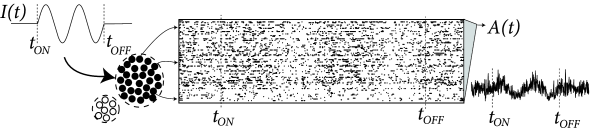
\includegraphics[width=0.8\linewidth]{x285.png}
	\caption{ Response of population to a signal $I(t)$, represented by a sinusoidal modulation of the input starting at $t_{ON}$ and ending at $t_{OFF}$, stimulates the population of $8 000$ excitatory neurons in a randomly coupled network of $8 000$ excitatory and $2 000$ inhibitory neurons (left). Each neuron produces a spike train (middle) illustrated here by lines of dots, each dot corresponding to a spike. Only $1\%$ of the population is shown. At the macroscopic level, the population activity $A(t)$ (right) counts spikes in time bins of $1$ ms averaged over the $8 000$ excitatory neurons. [\cite{GerKis14}] }
	\label{fig:x285}
\end{figure}

In this project we consider a large homogeneous population of neurons modeled by time dependent renewal process. A common approach to recover the activity of such a population is based on the refractory density [\cite{Ger00}, \cite{ChiGra07}, \cite{ChiGra08}, \cite{SchDeg17}]. But the integral formulation present in the refractory density equation makes this approach computationally inefficient and limit the analytical tractability. Therefore the goal of this work is to derive a low-dimensional population dynamics of spiking neurons, starting from a spectral expansion of the refractory density equation. Thus we will first introduce in Sections \ref{sec:renew} and \ref{sec:refractory}, renewal processes and the refractory density approach. Then we will recall some properties of the spectral expansion in Section \ref{sec:spect}, which in previous studies was used to approximate the dynamics of spiking networks, taking as state variable the membrane potential $v$ [\cite{MatGiu02}, \cite{SchOst13}, \cite{AugLad17}].


\section{Renewal processes} %spiking neuron model}
\label{sec:renew}

 %Hazard function: rate at t given last spike at t
%Survivor function: probability of no spike in [t ,t ˆ ]
%Interspike-interval density: probability densityof next spike at t given last spike at t P = ρS


A neuron model tells how an input is transformed into output spikes. We define $h(t)$ as the input potential, its time derivative is given by

\begin{equation}
\label{eq:h}
\tau_m\dot{h}=-h+\mu(t) +RI_{syn}(t)
\end{equation}

where $\mu(t)$ represents an external stimulus, and $I_{syn}$ is the synaptic current, due to the spikes from other neurons.

Renewal processes keep memory of the last event,i.e. the last firing time $\hat{t}$. The age, i.e the time elapsed since the last spike $\tau=t-\hat{t}$, is a state variable of the neuron. For those processes the spikes are generated according to a stochastic intensity called the hazard rate $\rho(\tau,h)$. The hazard rate $\rho(\tau,h)$ define the probability to spike between $t+\Delta t$ knowing that there were no spike between $t$ and $\hat{t}$

To generate a spike train according to the hazard rate $\rho(\tau,h)$ in a simulation, one would proceed as follows
\begin{itemize}
\item At each time step $\Delta t$ knowing the age $\tau$ of the neuron and the current input potential $h(t)$ the probability of a neuron to spike would be given by \begin{equation}
p_{spike}=1-\exp(-\rho(\tau,h)\Delta t)
\end{equation} We see that the probability to spike is $0$ for $\rho(\tau,h)=0$ and goes to $1$ for $\rho(\tau,h)\rightarrow +\infty$
\item When the neuron spikes, the age is reset to $0$, otherwise the age variable would be incremented by $\Delta t$. 
\end{itemize}


\subsection{Interval distribution and Survivor function}

Let us in this section assume a time-homogeneous process, i.e. $h=const$. We can calculate the interspike interval (ISI) density $P(\tau,h)$ i.e the probability to spike at age $\tau$. 

\begin{equation}
\label{eq:Pnorm}
\int_0^\infty P(\tau,h)\dd\tau=1 
\end{equation}

The interval distribution $P(\tau,h)$ is a probability density, which implies that integration of $P(\tau,h)$ over age yields a probability. The probability that a neuron which has fired a spike at $\hat{t}$ and fires the next spike between $\hat{t}$ and $t$ is given by $\int_0^\tau P(s,h) \dd s$.

The interspike-interval (ISI) distribution can be linked to the survivor function
\begin{equation}
\label{eq:S1}
S(\tau,h)=1-\int_0^\tau P(s,h) \dd s
\end{equation}

The survivor function $S(\tau,h)$ defines the probability that a neuron reaches the age $\tau$, so that a neuron "survive" without firing between $\hat{t}$ and $t$. $P(\tau,h)$ describes the probability to spike at age $\tau$. There it can be expressed as the product of the probability to survive until age $\tau$ times the momentary hazard $\rho(\tau,h)$. 

\begin{equation}
\label{eq:P2}
P(\tau,h)=\rho(\tau,h)S(\tau,h)
\end{equation}

The derivation of Eq.\eqref{eq:S1} yields to 

\begin{equation}
\label{eq:P3}
P(\tau,h)=-\frac{\dd}{\dd \tau}S(\tau,h)
\end{equation}

Inserting Eq.\eqref{eq:P2} in Eq.\eqref{eq:P3}, we find that the hazard rate $\rho(\tau,h)$ corresponds to the rate of decay of the survivor function

\begin{equation}
\label{eq:ratedecays}
\rho(\tau,h)=-\frac{\frac{\dd}{\dd \tau}S(\tau,h)}{S(\tau,h)}
\end{equation}

Integrating eq.\ref{eq:ratedecays} yields to the survivor function
\begin{equation}
\label{eq:S2}
S(\tau,h)=\exp\big[-\int_0^\tau\rho(s,h)\dd s\big]
\end{equation}

Inserting Eq.\eqref{eq:S2} in Eq.\eqref{eq:P2} the interval distribution can be explicitly express in terms of the hazard, and is by itself normalized

\begin{equation}
\label{eq:P4}
P(\tau,h)=-\frac{\dd}{\dd \tau}S(\tau,h)=\rho(\tau,h)\exp\big[-\int_0^\tau\rho(s,h)\dd s\big]
\end{equation}

Each of the three function $\rho(\tau,h)$, $P(\tau,h)$ and $S(\tau,h)$ is sufficient to describe statistical properties of a renewal system.

\subsection{Examples }

Interval distribution and hazard functions have been measured in many experiments. Here are some examples that will be useful for finding analytical approximations and/or that agree  with experimental measurements.

\subsubsection{Simple model with recovery function}

\begin{figure}[h!]
	\centering
	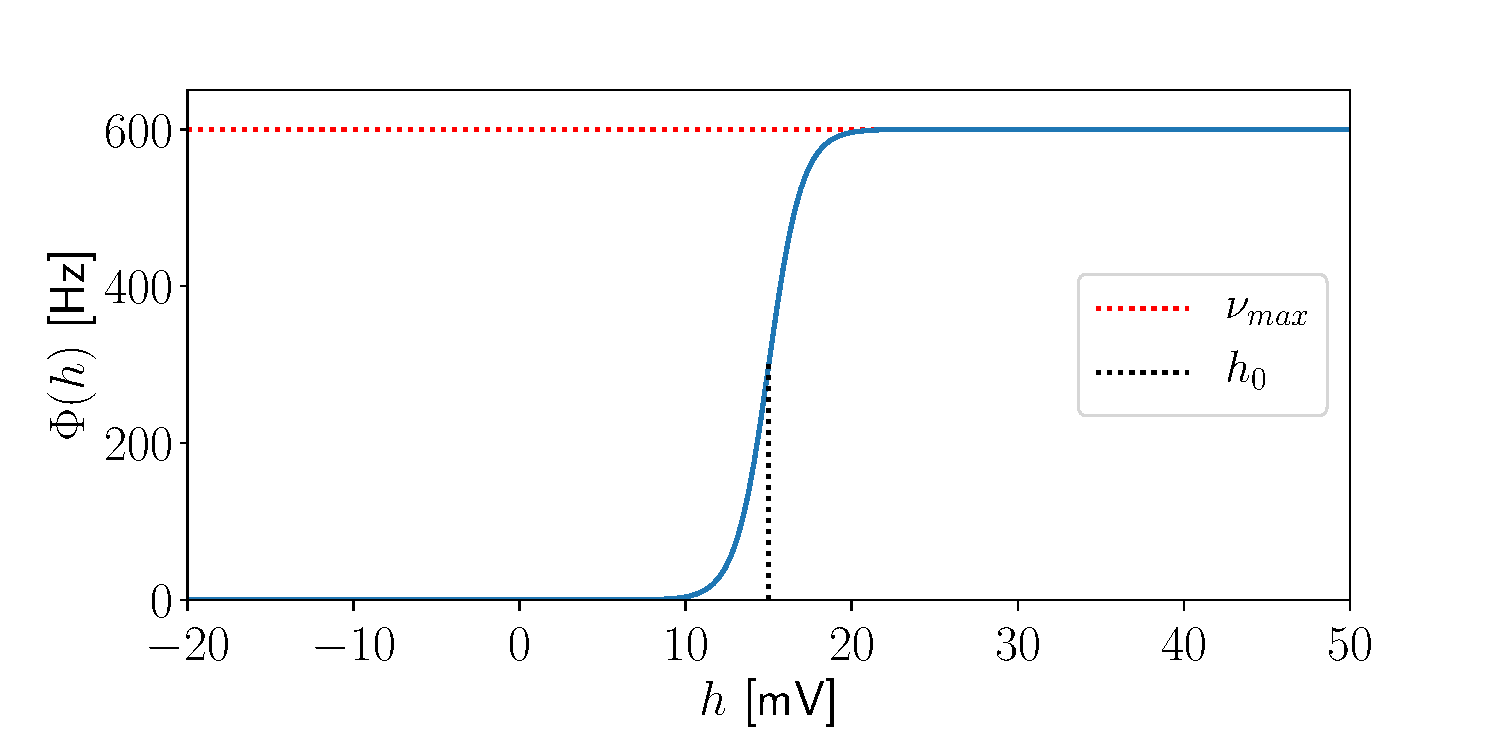
\includegraphics[width=0.8\linewidth]{phi_h.pdf}
	\caption{ Rate $\Phi(h)$ as a function of input potential $h$. With $h_0=15$ mV , $\beta=1$ mV$^{_1}$ and $\nu_{max}=0.6$ kHz.}
	\label{fig:phi_h}
\end{figure}


\begin{figure}[h!]
	(a) \\
	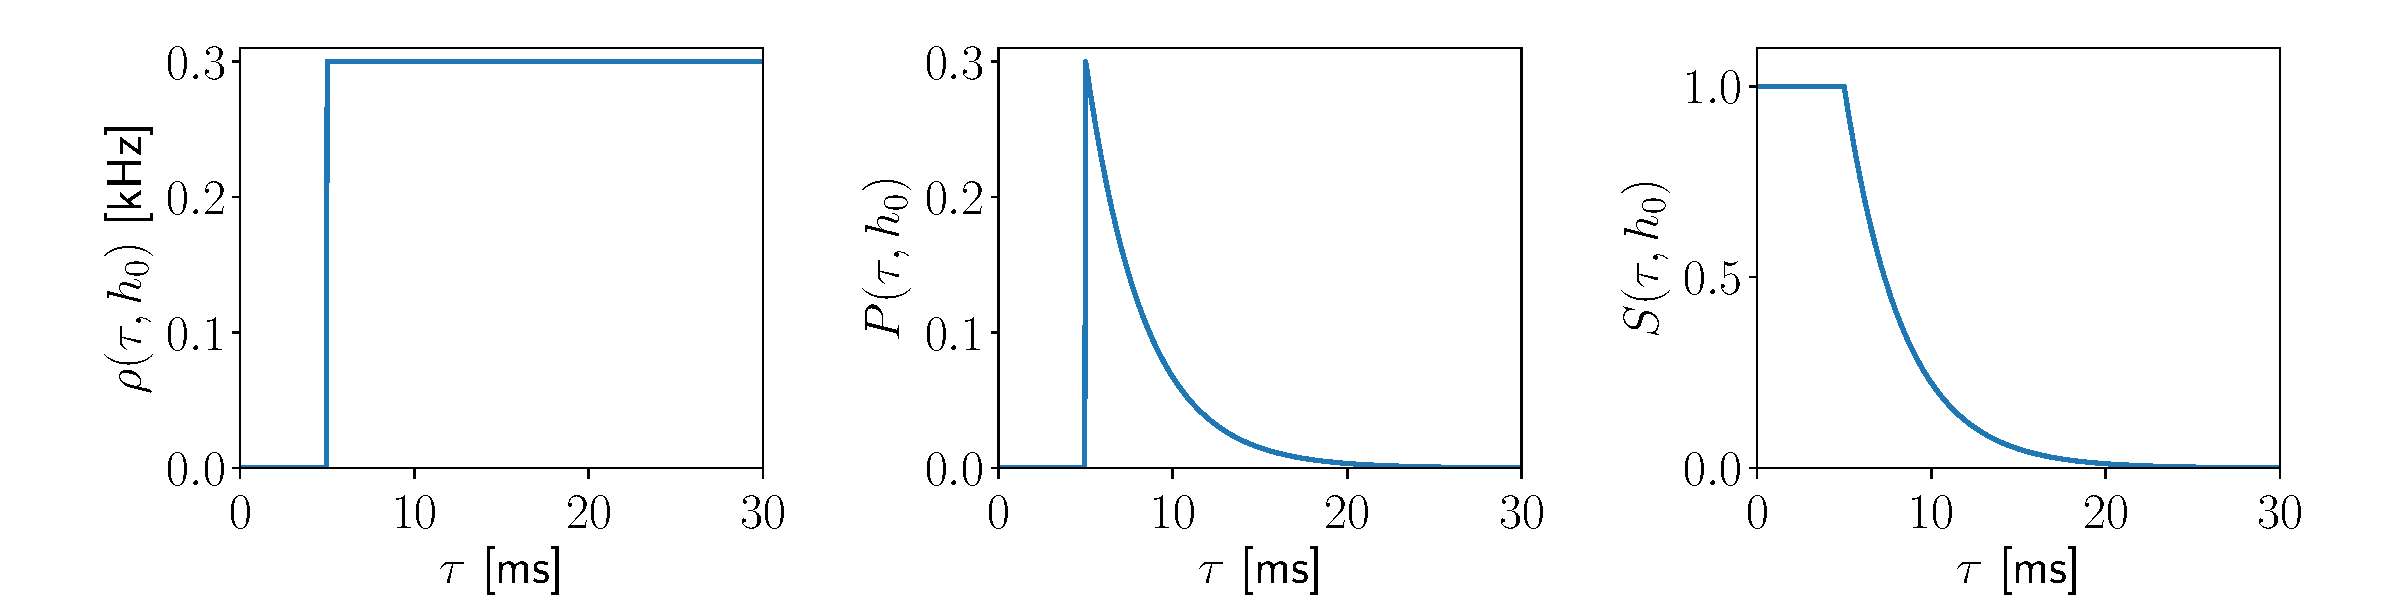
\includegraphics[width=\linewidth]{poissonRHOSP.pdf}
	(b)\\
	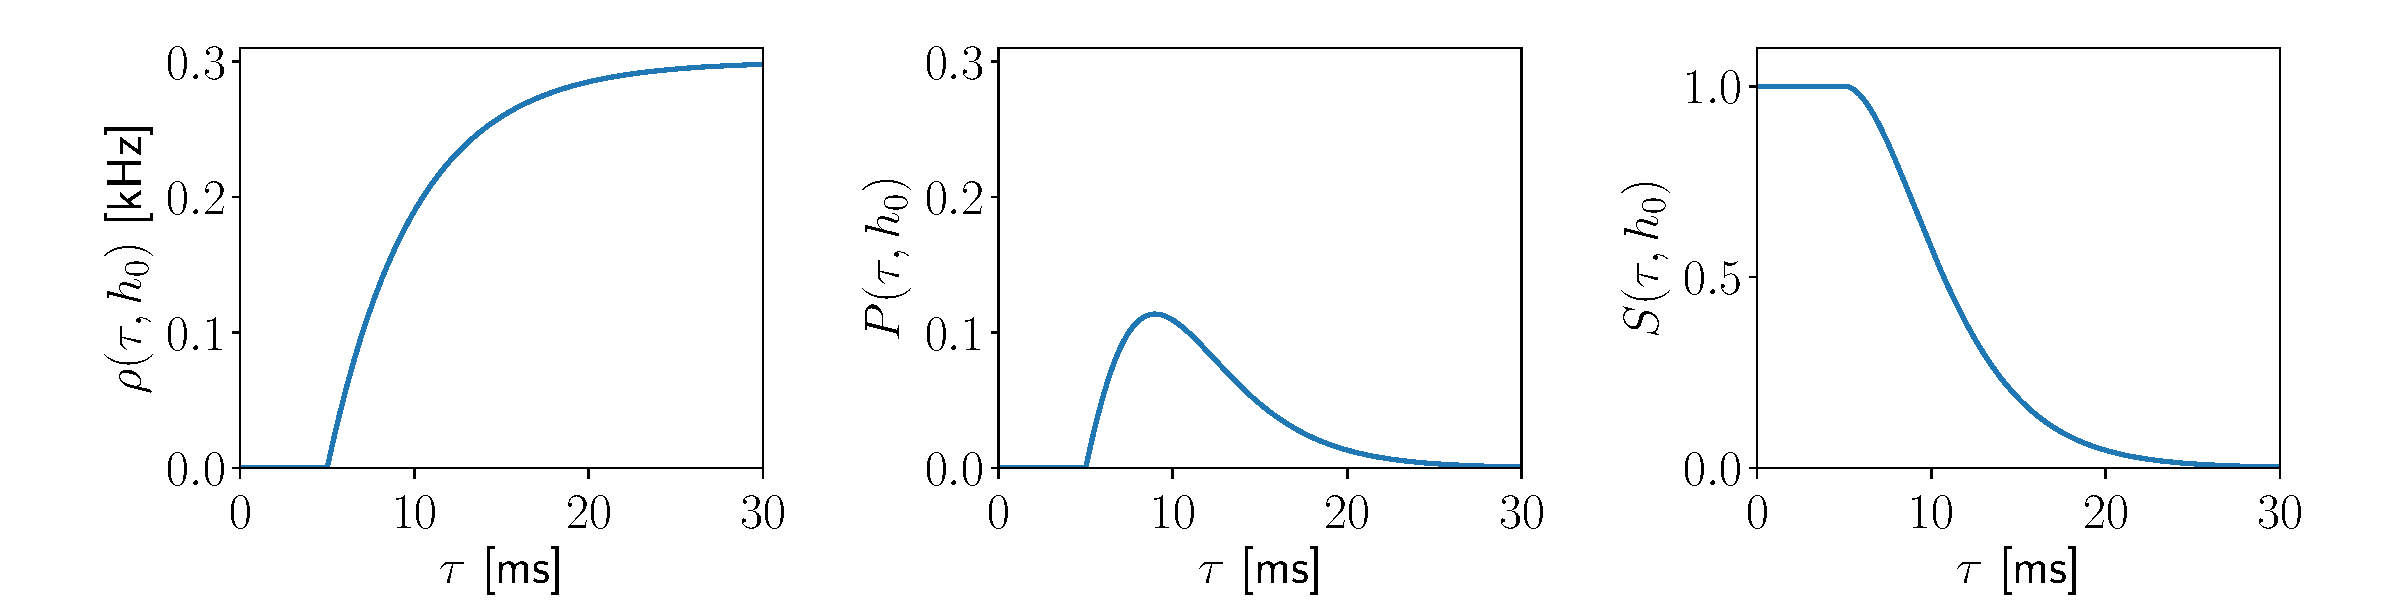
\includegraphics[width=\linewidth]{expRHOSP.pdf}
	\caption{Hazard rate $\rho(\tau,h)$ (left), interval distribution $P(\tau,h)$ (middle) and survivor function $S(\tau,h)$ (right) for different recovery function $g(\tau)$. (a) Recovery function for a Poisson neuron with absolute refractoriness $\Delta$, with $\Delta=5$ ms, $h=h_0$, $\nu_{max}=600$ Hz.  (b) Recovery function defined  by Eq.\eqref{eq:expabs} with $\Delta=5$ ms, $h=h_0$, $\nu_{max}=600$ Hz.  }
	\label{fig:renewalprocess}
\end{figure}
%In the previous section we were implicitly considering stationary renewal system using the notation $\rho(t|\hat{t})$.

The hazard rate, can be expressed as a product of the instantaneous rate $\Phi(h)$ with a recovery function $g(\tau)$

\begin{equation}
\label{eq:rho}
\rho(\tau,h)=\Phi(h)g(\tau)
\end{equation}

The function $\Phi(h)$ is a monotonically increasing function. In our examples we will use a sigmoidal function with threshold $h_0$ illustrated on Fig.\ref{fig:phi_h}. For $h>>h_0$ the firing rate goes to the value $\nu_{max}$ for $h<<h_0$ it goes to $0$.

\begin{equation}
\label{eq:phi}
\Phi(h)=\frac{\nu_{max}}{1+\exp[-\beta(h-h_0)]}
\end{equation}


The hazard rate, the survival probability, and the interval distribution are shown in Fig.\ref{fig:renewalprocess} for two examples of recovery function $g$, with potential $h=h_0$ i.e $\Phi(h)=\frac{\nu_{max}}{2}$. Fig.\ref{fig:renewalprocess}(a) corresponds to a Poisson process with absolute refractory period $\Delta$: 
\begin{equation}
\label{eq:poissonabs}
g(\tau)=\theta(\tau-\Delta)
\end{equation}

$\theta(\tau-\Delta)$ denotes the Heaviside function. The recovery function for Fig.\ref{fig:renewalprocess}(b) is given by
\begin{equation}
\label{eq:expabs}
g(\tau)=\left[1-\exp(-\eta(\tau-\Delta))\right]\theta(\tau-\Delta)
\end{equation}

The main difference is that for the Poisson neuron with absolute refractoriness the recovery function Eq.\eqref{eq:poissonabs} make a jump, whereas in Eq.\eqref{eq:expabs} the transition is smooth which gives rise to relative refractoriness. The time course of the recovery function given by Eq.\eqref{eq:expabs}, approximate well the recovery function measured for auditory neurons of the guinea-pig [\cite{Prij93}]


\subsubsection{Gamma neuron model}

The gamma neuron model is often used to model spike trains as it is one of the easiest non-Poisson process to analyze. For this neuron model the interspike distribution is given by

\begin{equation}
\label{eq:gamma}
P(\tau)=\frac{\beta^\gamma}{\Gamma(\gamma)}\tau^{\gamma-1}e^{-\beta\tau}
\end{equation}

Where $\beta:=\beta(h)$ is a rate which depend on the input potential $h$

\begin{figure}[h!]
	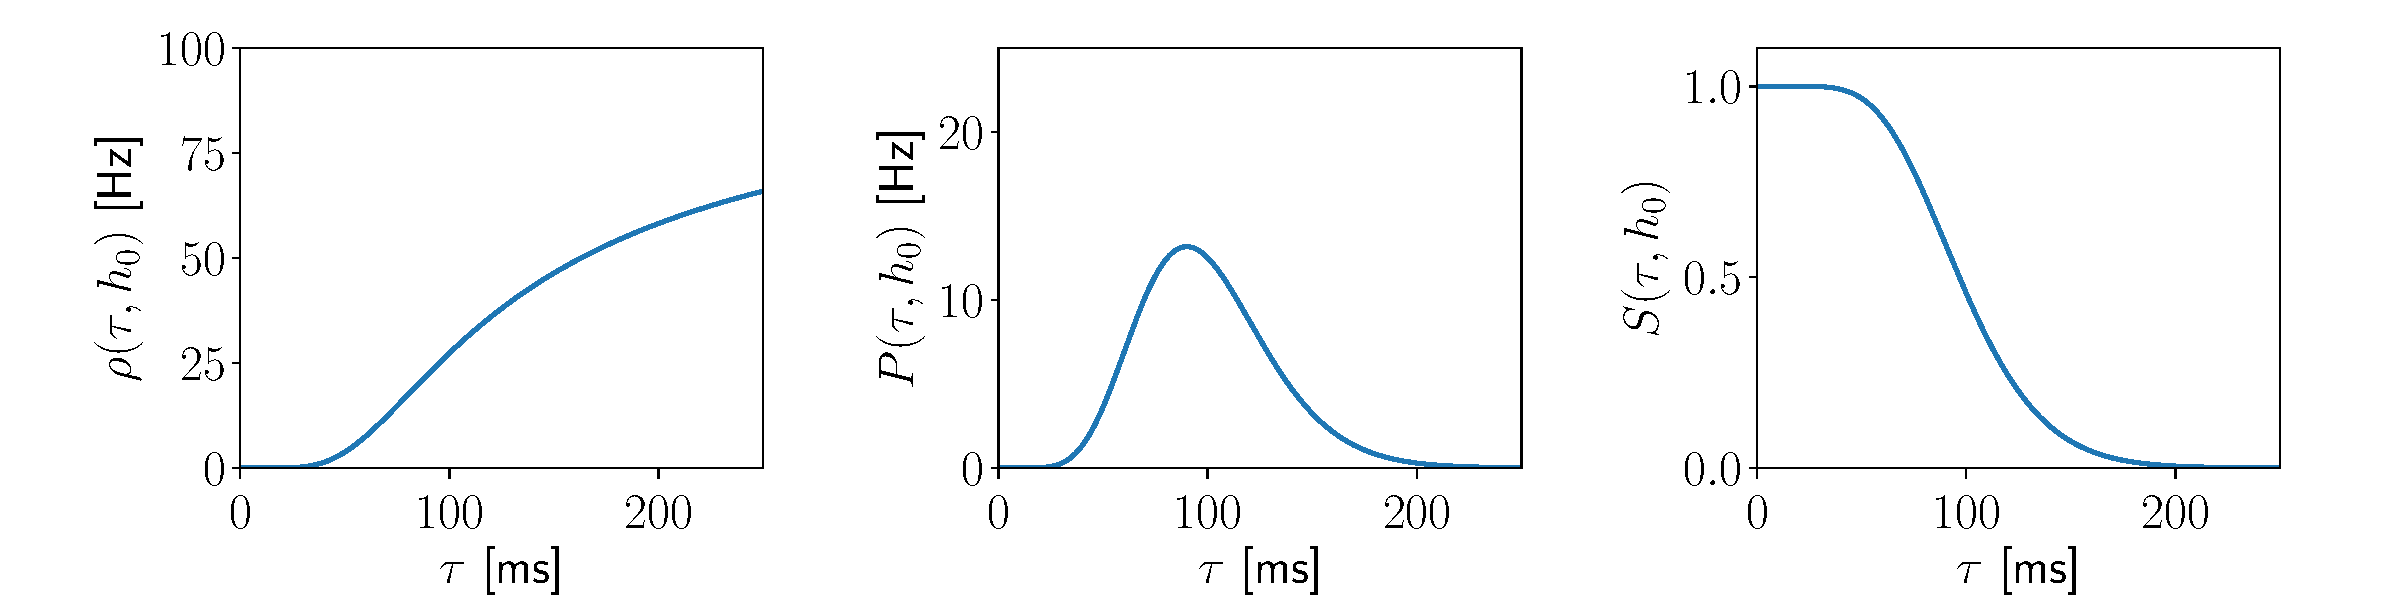
\includegraphics[width=\linewidth]{gamma.pdf}
	\caption{\textbf{Gamma neuron model.} Hazard rate $\rho(\tau,h)$ (left), interval distribution $P(\tau,h)$ (middle) and survivor function $S(\tau,h)$ (right) for a Gamma neuron model with $\beta=100$ Hz and $\gamma=10$ }
	\label{fig:gammaprocess}
\end{figure}

The rate of this neuron model is $R=\beta/\gamma$, And the coefficient of variation is given by $C_V=\gamma^{-\frac{1}{2}}$. For $\gamma=1$ this corresponds to a Poisson process. For $C_V>1$ the interspike distribution diverges as $\tau$ goes to $0$. One can see the gamma neuron model as a succession of $\gamma$ states where each state is  a Poisson neuron with firing rate $\beta$ since one has to pass by each state before spiking, this implies that the global rate of the total chain is $R=\beta/\gamma$, and induces relative refractoriness as shown on Fig.\ref{fig:gammaprocess}.


\subsubsection{Perfect integrate-and-fire model driven by white noise}
\label{sec:pif}


\begin{figure}[h!]
	\centering
	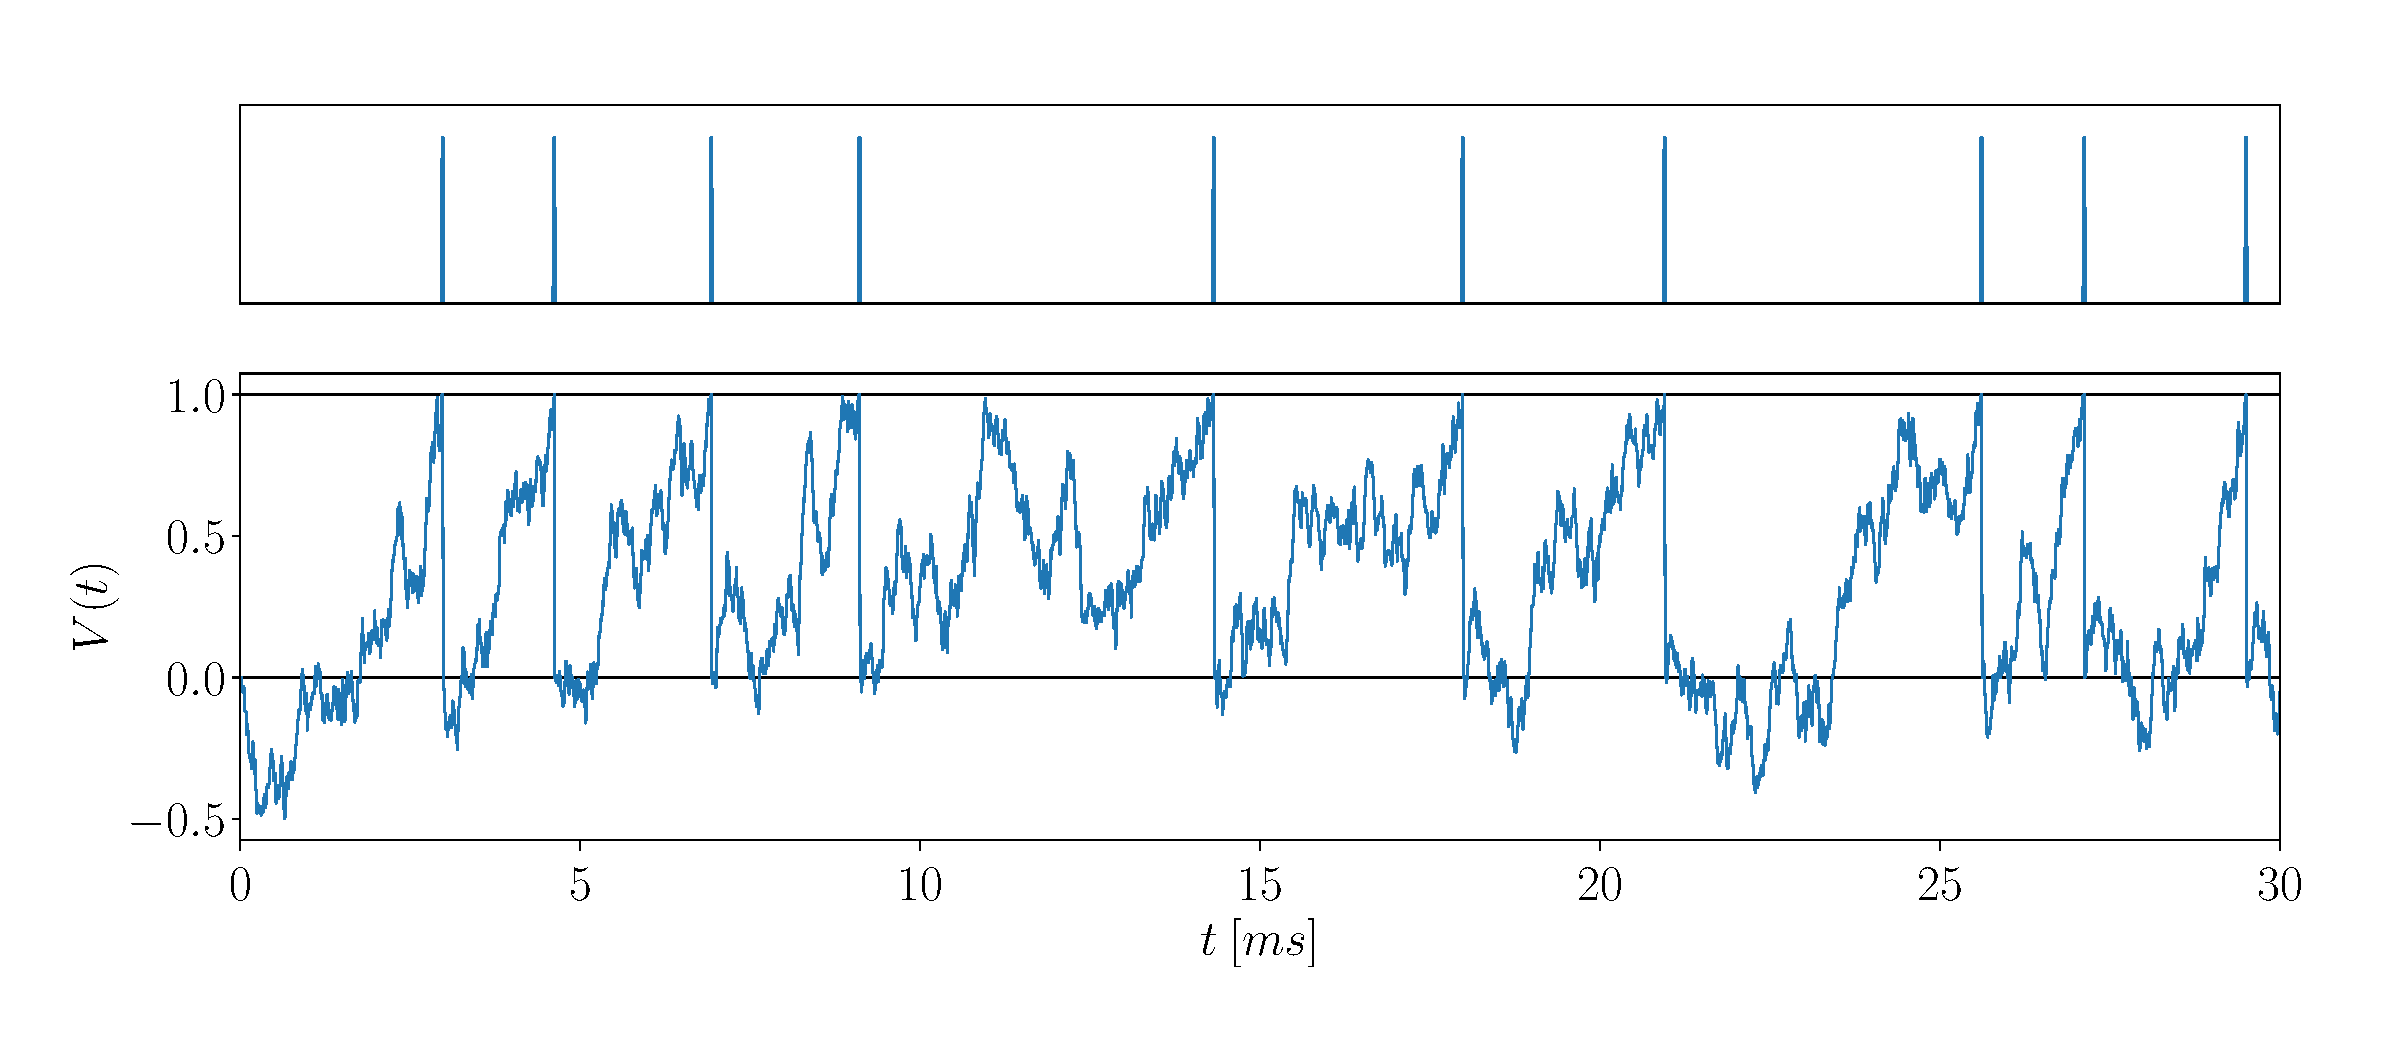
\includegraphics[width=0.8\linewidth]{PIF_V}
	\caption{Typical realization $V(t)$ for the PIF model driven with a white noise with  $f(h)=0.3$ $V_{th}$, $D=0.1$ $V_{th}^2$,$\tau_v=1$ ms $V_{th}=1$. The generated spike train is indicated on the top. 
	}
	\label{fig:PIFV}
\end{figure}


\begin{figure}[h!]
	
	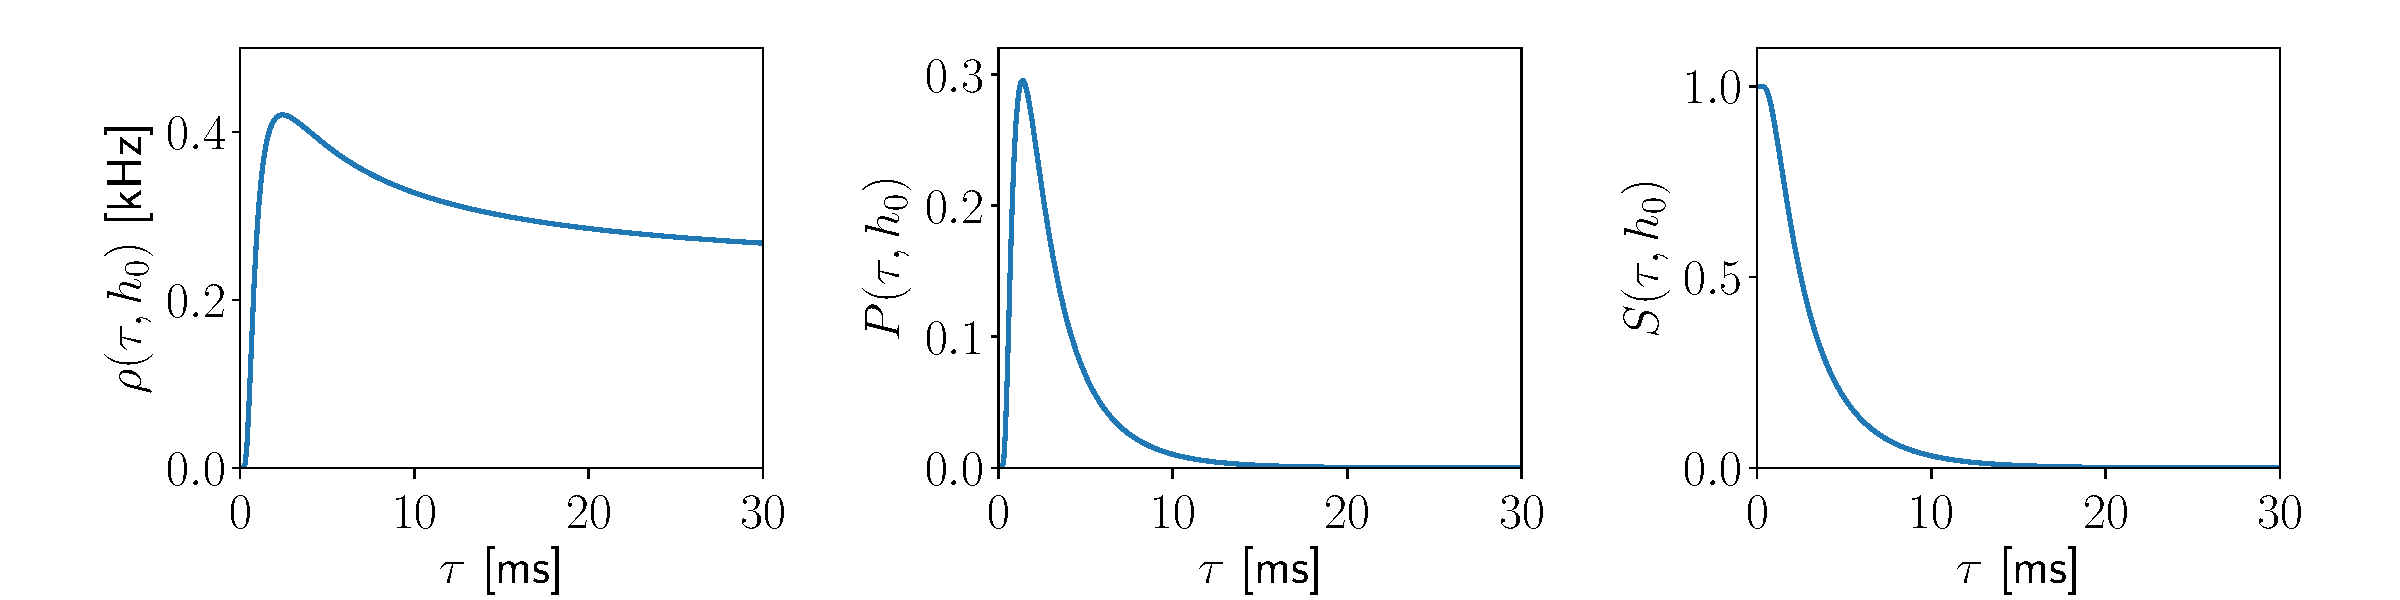
\includegraphics[width=\linewidth]{inversegaussian.pdf}
	\caption{\textbf{PIF neurons.} Hazard rate $\rho(\tau,h)$ (left), interval distribution $P(\tau,h)$ (middle) and survivor function $S(\tau,h)$ (right) for the PIF model driven with a white noise with $f(h)=0.3$ $V_{th}$, $D=0.1$ $V_{th}^2$,$\tau_v=1$ ms $V_{th}=1$
	}
	\label{fig:inversegaussianprocess}
\end{figure}

The perfect integrating-and fire model has been used to explain statistics of isolated neurons. The membrane potential $V$ of a neuron can be seen as a Brownian-motion with drift $f(h)$ driven by a white noise, which is reset to the value $V_r$ when it hits the threshold $V_{th}$. The function $f(h)$ is a mean current which depends on the input potential $h$.

\begin{align}
\label{eq:Vxi}
\tau_v\dot V=f(h) +\sqrt{2D}\xi(t), \:\:\:\:\:\:\:\: \:\:\:\:\: if\:\:\:\:\:\:  V=V_{th}\:\:\:\:\:\:V\rightarrow V_r\\ 
\langle\xi(t)\xi(s)\rangle=\delta(t-s)
\end{align}

A typical realization of the dynamics of $V(t)$ for a single neuron and the corresponding spike train is illustrated on Fig.\ref{fig:PIFV}. The statistics of such neurons are shown on Fig.\ref{fig:inversegaussianprocess}.



For this neuron model the interspike distribution is given by

\begin{equation}
\label{eq:inversegaussian}
P(\tau,h)=\frac{V_{th}\tau_v}{\sqrt{4\pi D\tau^3}}\exp\left(-\frac{(f(h)\tau-V_{th}\tau_v)^2}{4D\tau}\right)
\end{equation}

The rate of this neuron model is $R=\frac{f(h)}{V_{th}\tau_v}$, And the coefficient of variation is given by $C_V=\sqrt{\frac{2D}{\tau_vf(h)V_{th}}}$.



\section{Moment of the interspike interval distribution $P(\tau)$}

For the upcoming theoretical derivations, it is usefull to introduce the moment of the interspike interval distribution. For a stationary spike train, the ISI distribution is also stationary. Here  $h$ is constant, so we used the notation $P(\tau)$ instead of $P(\tau,h)$.  The interval distribution allows to compute the $k-$th moment,

\begin{equation}
\label{eq:Pmoment}
\langle\tau^k\rangle=\int_0^\infty \tau^kP(\tau)\dd\tau
\end{equation}

It is useful to introduce the Laplace transform
\begin{equation}
\label{eq:Plaplace}
P_L(\lambda)=\int_0^\infty\dd\tau e^{-\lambda \tau}P(\tau)
\end{equation}

from which the  $k-$th ISI moment can be generated

\begin{equation}
\label{eq:Pmoment2}
\langle\tau^k\rangle=(-1)^k\frac{\dd^k P_L}{\dd \lambda^k}\Bigr|_{\lambda=0}
\end{equation}

Hence, $P_L(\lambda)$ is called the ISI moment generating function. We can generated from this function the ISI cumulants defined by

\begin{equation}
\label{eq:Pcumulant}
\kappa_k=(-1)^k\frac{\dd^k \ln P_L}{\dd \lambda^k}\Bigr|_{\lambda=0}
\end{equation}

The first two ISI cumulants are related to the ISI moments by
\begin{align}
\label{eq:kappa1234}
\kappa_1&=\langle\tau\rangle\\
\kappa_2&=\langle\tau^2\rangle-\langle\tau\rangle^2
\end{align}

%\kappa_3&=<\tau^3> -3<\tau^2><\tau>+2<\tau>^3\\
%\kappa_4&=<\tau^4>-4<\tau^3><\tau>-3<\tau^2>^2+12<\tau^2><\tau>^2-<\tau>^4\\
%\end{align}

The cumulants can be used to characterize the shape of the ISI density. The rate of a process $R$ is given by
\begin{equation}
\label{eq:R}
R=\langle\tau\rangle^{-1}=\kappa_1^{-1}
\end{equation}

An important measure that quantify the variability of ISI distribution is the coefficient of variation $C_V$ defined as


\begin{equation}
\label{eq:CV}
C_V=\sqrt{\frac{\langle\tau^2\rangle}{\langle\tau\rangle^2}-1}=\frac{\sqrt{\kappa_2}}{\kappa_1}
\end{equation}

A Poisson process produces distributions with $C_V=1$ which indicate a highly irregular spike train. A value of $C_V>1$, implies that a given spike train is less regular than a Poisson process with the same firing rate. If $C_V<1$, then the spike train is more regular. Whereas $C_V=0$ indicates a perfectly regular spike train.


\section{Populations of neurons and refractory density equations}
\label{sec:refractory}
\subsection{Population model}

There are about a hundred billion neurons in the human brain, distributed in different brain area and which form elaborate neural networks. Within a brain area one can identify subregions and layers where neurons are organized in populations of cells with similar properties. Eloquent examples are barrel columns in the primary somatosensory cortex [\cite{Lef09}], and pools of motor neurons [\cite{KanSch00}].

Given the large number of neurons in a population, rather than tracking the spiking of individual neurons,  it is appealing to describe the mean activity. Fig.\ref{fig:x285} illustrate the transition from a microscopic to a macroscopic description. The theory of population dynamics dates back to the 1970s [\cite{Kni72}, \cite{WilCow72}] and modern variants are used to predict the temporal evolution of the activity $A(t)$ [\cite{SchDeg17}]. In a network of $N$ neurons the population activity $A(t)$ is defined as the proportion of active neuron. Denoting by $t^f_j$ the firing time $f$ of the neuron $j$, the activity can be expressed as
\begin{equation}
A(t)=\frac{1}{N}\sum_{j=1}^N\sum_f\delta(t-t_j^f)
\end{equation}

%$A(t)=lim_{\Delta t \rightarrow 0} \frac{1}{\Delta t}\frac{n_{act}(t;t+\Delta t)}{N}$

where $\delta$ a dirac function.


We consider large homogeneous population of neurons i.e all neuron are identical and receive the same input potential, composed of an external input$\mu(t)$ and a synaptic input current $I_{syn}$, due to the spikes from other neurons.

\begin{equation}
\label{eq:input}
RI_{syn}(t)=JA(t)
\end{equation}

where $J$ denotes the coupling constant with the units of voltage seconds. For the sake of simplicity we will consider all-to-all coupling, i.e. each neuron is coupled to each neuron and therefore receives the same input proportional to the mean activity.

\subsection{Refractory density equation}
\label{secrefde}

% TODO Wchange ? 
An approach on the refractory density $q(\tau,t) $ let analyze the dynamic in an homogeneous population [\cite{GerKis02}]. $q(\tau,t)$ characterize the number of neuron at time $t$ that are in a similar state of activity, i.e with age $\tau=t-\hat{t}$, where $\hat{t}$ is the last spike time of the neuron. The population activity is thus given by
\begin{equation}
\label{eq:A}
A(t)=q(0,t)
\end{equation}

As long as a neuron does not fire, the age $\tau$ increase at the speed of $\frac{\dd \tau}{\dd t}=1$, therefore the flux along the refractory variable $\tau$ is simply $q(\tau,t)$ and the continuity equation is given by

\begin{equation}
\label{eq:continuity1}
\frac{\partial q}{\partial t}=-\frac{\partial q}{\partial \tau}
\end{equation}

When a neuron fires, the trajectory along the refractory variable $\tau$ stops at the current value and "reappears" at $\tau=0$. The instantaneous probability to fire is given by the hazard function $\rho(\tau,h)$.Therefore the loss per unit time is given by $-\rho(\tau,h)q()\tau,t)$ and the full dynamic is then given by the master equation:

\begin{equation}
\label{eq:masterequation}
\partial_t q(\tau,t)=-\partial_\tau q(\tau,t)-\rho(\tau,h)q(\tau,t)
\end{equation}

% \textcolor{red}{$q(\tau_i)\rho(\tau_i)\Delta t$}
%  \textcolor{blue}{$q(\tau_{i+1},t_{j+1})=q(\tau_i,t_j)[1-\rho(\tau_i)\Delta t]$}
%  \textcolor{blue}{$\frac{q(\tau_{i+1},t_{j+1})-q(\tau_i,t_j)}{\Delta t}=-\rho(\tau_i)q(\tau_i,t_j)$}

The dynamics is schematized on Fig.\ref{fig:qtau}. At time $t_j$ The proportion of neurons at age $\tau_i$ which are firing and will reappear at age $0$, is given by $q(\tau_i,\tau_j)\rho(\tau_i,h_j)\Delta t$ (red arrow). The neuron that did not fire will reach the age $\tau_{i+1}$ at time $t_{j+1}$ (blue arrow). The sum of all trajectories that "disappear" at time $t$ due to firing, are "reappearing" at $\tau=0$ since each neuron will fire at some finite time, the boundary conditions are

\begin{align}
\label{eq:boundarycondition}
q(0,t)&=\int_{0}^{\infty}\rho(\tau,h)q(\tau,t)d\tau=A(t) \\
q(\infty,t)&=0
\end{align}

\begin{figure}[h!]
	\centering
	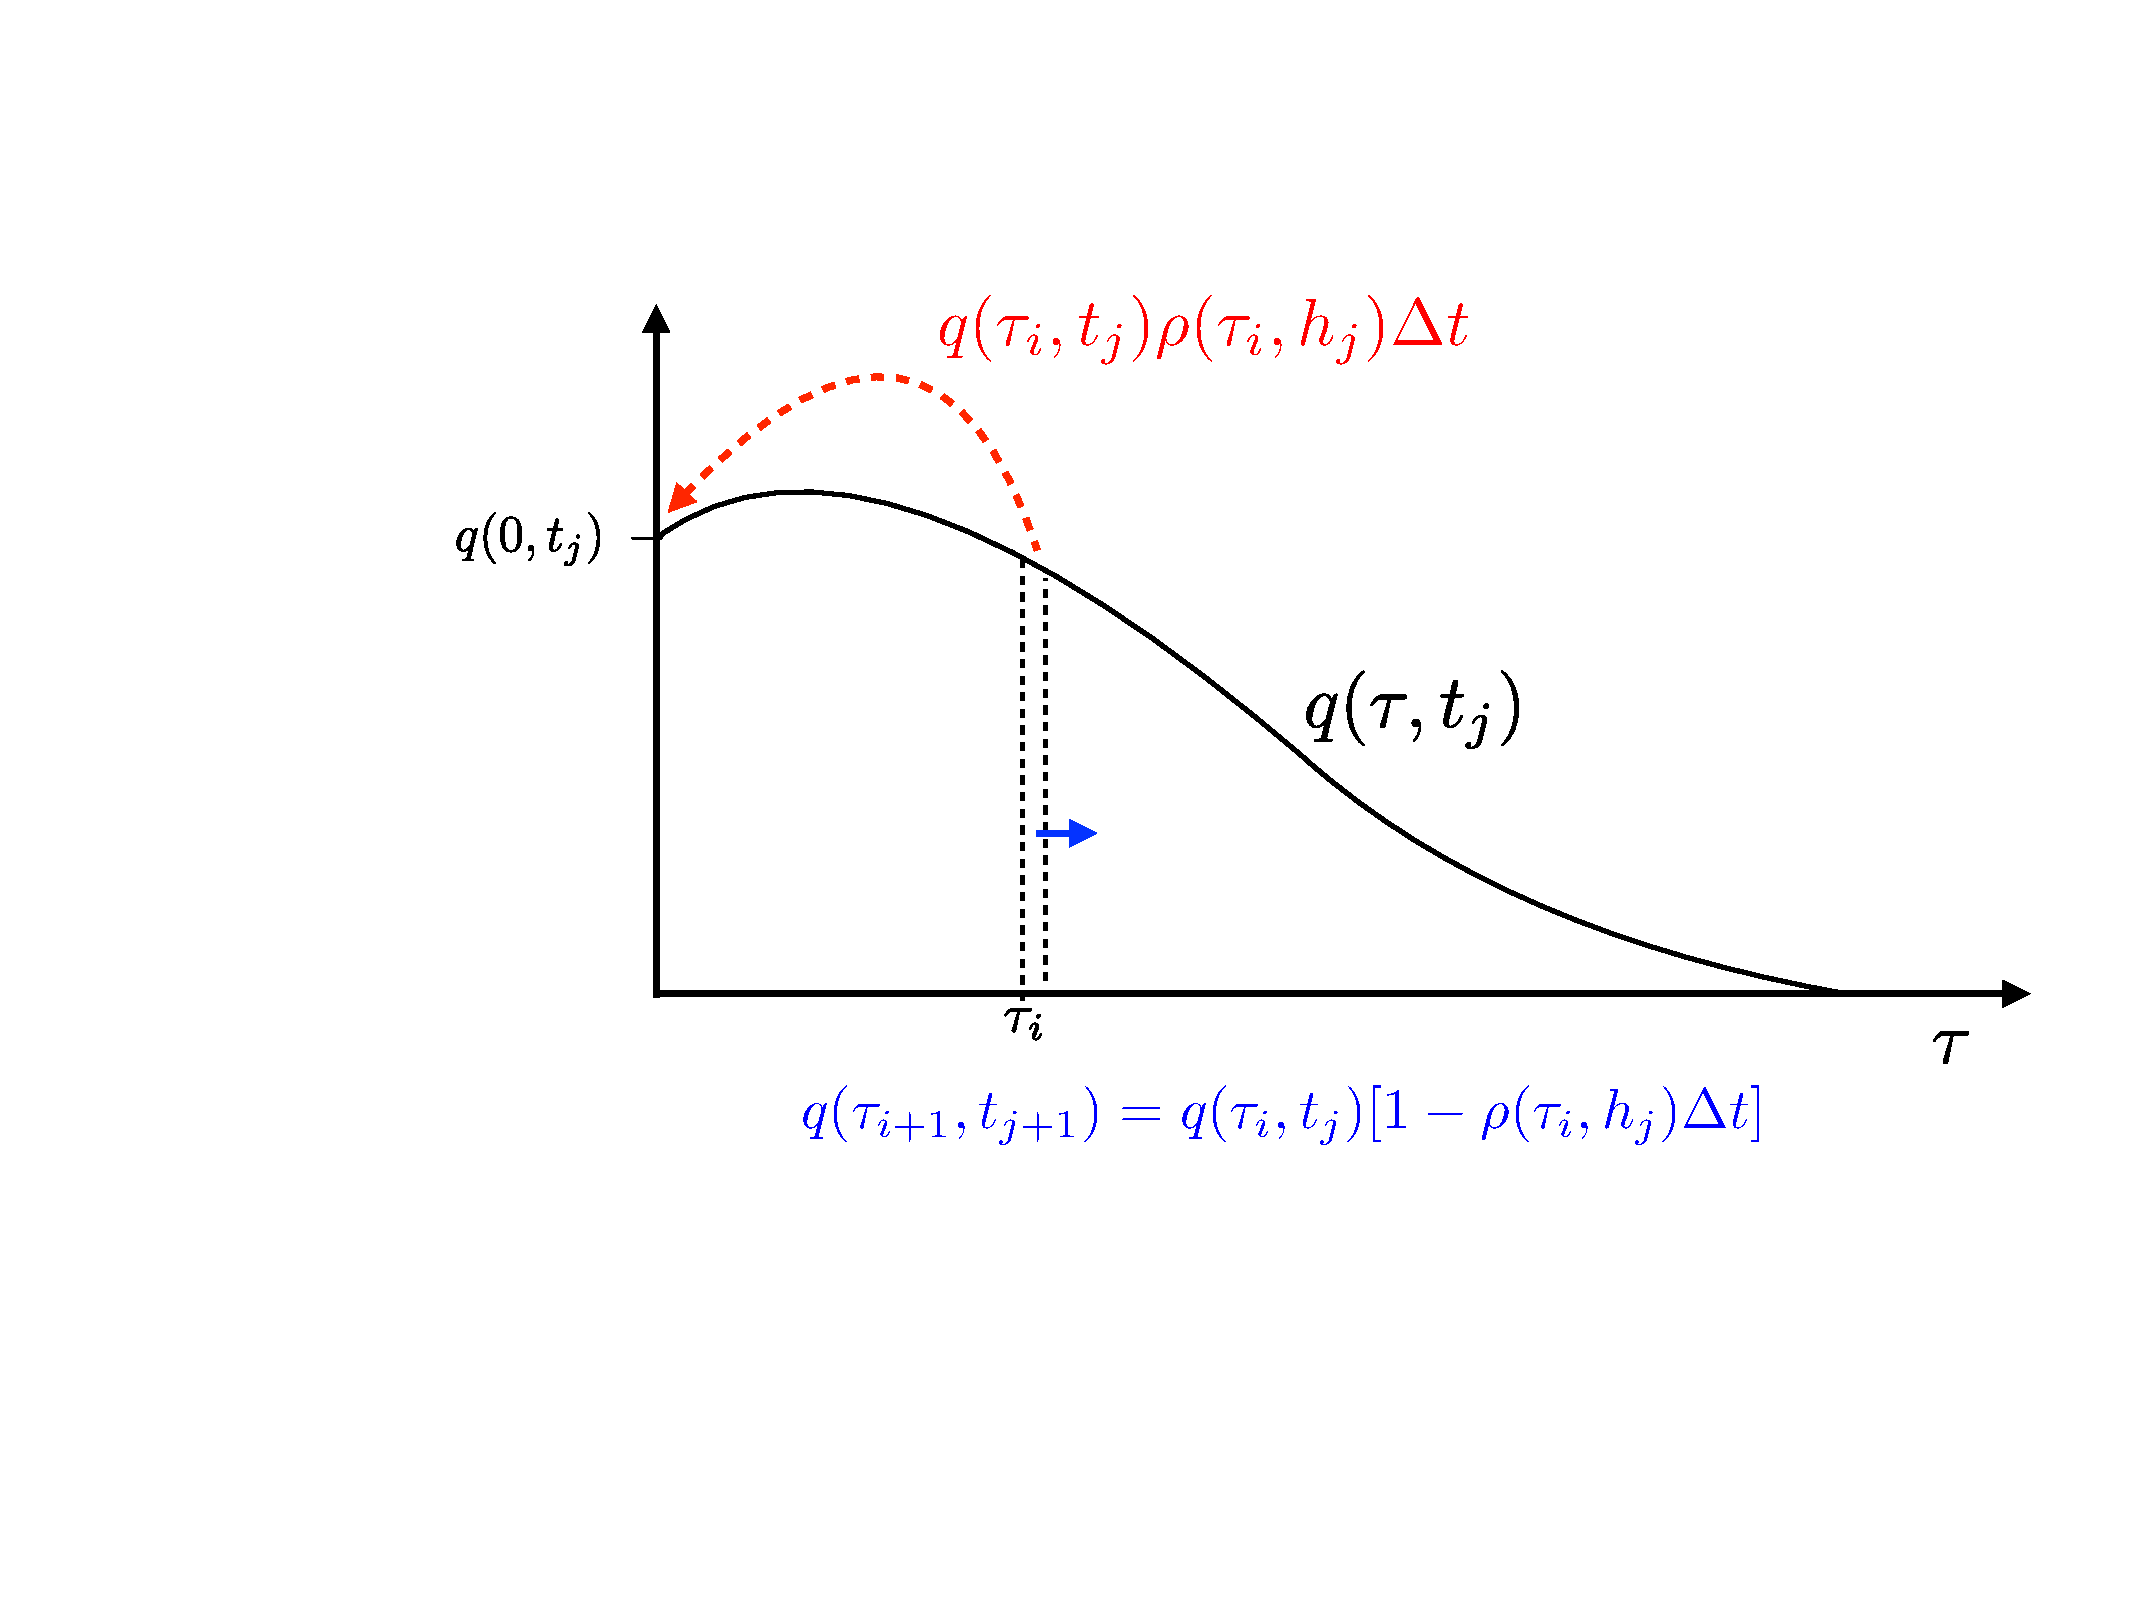
\includegraphics[width=0.7\linewidth]{qtau.pdf}
	\caption{Scheme of refractory density dynamics. The red arrow represents the proportion of neurons with age $\tau_i$ whose fire at time $t_j$, the blue one represents those that are not firing and will reach the age $\tau_{j+1}$ at time $t_{j+1}$. Taking the limit $\Delta t \rightarrow 0$ yields to Eq.\eqref{eq:masterequation}
	}
	\label{fig:qtau}
\end{figure}

Additionally, $q$ is normalized

\begin{equation}
\label{eq:qnormalisation}
\int_0^\infty q(\tau,t)\dd \tau = 1
\end{equation}

and has the initial density

\begin{equation}
\label{eq:qinitial}
q(\tau,0)=q_0(\tau)
\end{equation}

where $q_0(\tau)$ is some function that satisfies the conditions Eq.\eqref{eq:boundarycondition} and Eq.\eqref{eq:qnormalisation}.


\section{Spectral decomposition method}
\label{sec:spect}


We apply a probability density approach, which describes the evolution of the density of states $q(x,t)$, in the phase space of a specific choice of neuronal state variable $x$.
Many approaches consider only one state, the membrane potential $v$, governed by the integrate and fire model. In the refractory density approach, the state variable is the age $\tau$, i.e the time elapsed since the last spike. Assuming that the state variable $x$ can be described by a Markovian dynamics, we can write down an evolution equation for the state density $q$ in the following form

\begin{equation}
\label{eq:generaleq}
\partial_t q(x,t)=\mathcal{L}q(x,t)
\end{equation}

Where $\mathcal{L}$  is the evolution operator. Taking the membrane potential $v$ as a state variable the evolution operator corresponds to the Fokker-Planck operator [\cite{MatGiu02},\cite{SchOst13}]. We will first recall some property for a general evolution operator.



\subsection{General properties of the evolution operator}
The operator $\mathcal{L}$ of Eq.\ref{eq:generaleq} has a set of eigenfunctions and associated eigenvalues
\begin{equation}
\label{eq:fokkerplanckoperator}
\mathcal{L}\ket{\phi_n}=\lambda_n\ket{\phi_n}
\end{equation}

Where $\ket{\phi_n}=\phi_n(x,t)$ and $\lambda_n=\lambda_n(t)$.
The time dependency provides a moving basis $\{\ket{\phi_n}\}$. 

Because $\mathcal{L}$ is a real operator, if an eigenvalue $\lambda_n$ is complex, its complex conjugate $\bar{\lambda}_n$  is also an eigenvalue of $\mathcal{L}$, with eigenfunction $\ket{\bar{\phi_n}}$. We will use the notation $\bar{\lambda}_n=\lambda_{-n}$, i.e the sums over the spectrum of $\mathcal{L}$ range over all integer numbers. Note that $\lambda_0=0$ is always an eigenvalue of the operator $\mathcal{L}$ and corresponds to the stationary solution.

Because $\mathcal{L}$ is not generally Hermitian we also need to define the eigenfunctions $\ket{\psi_n}$ of the adjoint operator $\mathcal{L}^{+}$ 

\begin{equation}
\label{eq:fokkerplanckoperatordega}
\mathcal{L}^+\ket{\psi_n}=\tilde{\lambda}_n\ket{\psi_n}
\end{equation}

The adjoint operator is defined as $\langle\psi|\mathcal{L}\phi\rangle=\langle\mathcal{L}^+\psi|\phi\rangle$, where we introduce the inner product

\begin{equation}
\label{eq:innerproduct}
\langle\psi|\phi\rangle=\int\psi(x,t)\phi(x,t)\dd x
\end{equation}

Using the properties of the operator, one can show that the eigenvalues of Eq.\eqref{eq:fokkerplanckoperator} and Eq.\eqref{eq:fokkerplanckoperatordega} are the same

\begin{align}
\lambda_n\langle\psi_n|\phi_n\rangle &=\int\psi_n(x,t)\mathcal{L}\phi_n(x,t)\dd x  \nonumber \\
&=\langle\psi_n|\mathcal{L}\phi_n\rangle \nonumber \\
&=\langle\mathcal{L}^+\psi_n|\phi_n\rangle  \nonumber \\
&=\int\mathcal{L}^+\psi_n(x,t)\phi_n(x,t)\dd x \nonumber \\
&=\tilde{\lambda}_n\langle\psi_n,|\phi_n\rangle \label{eq:sameeig}
\end{align}

Eq.\eqref{eq:sameeig} implies that $\lambda_n=\tilde{\lambda}_n$ and

\begin{equation}
\label{eq:fokkerplanckoperatordega2}
\mathcal{L}^+\ket{\psi_n}=\lambda_n\ket{\psi_n}
\end{equation}

For different eigenvalues, the eigenfunctions $\psi_i$ and $\phi_j$ are orthogonal

\begin{align}
\lambda_j\langle\psi_i|\phi_j\rangle
&=\langle\psi_i|\mathcal{L}\phi_j\rangle \nonumber \\
&=\langle\mathcal{L}^+\psi_i|\phi_j\rangle  \nonumber \\
&=\lambda_i\langle\psi_i|\phi_j\rangle \label{eq:lorthogonal}
\end{align}

And with an appropriate normalization the two set of eigenfunctions are biorthonormal

\begin{equation}
\label{eq:dij}
\langle\psi_i|\phi_j\rangle=\delta_{ij}
\end{equation}

The density of state $q(x,t)$ can be expressed in terms of this basis

\begin{equation}
\label{eq:p}
\ket{q}=\sum_na_n\ket{\phi_n}
\end{equation}

where $a_n(t)=\langle \psi_n | q\rangle$ are the time dependent coefficients of the modal expansion. Since $q$ is real, $\bar{a}_n=a_{-n}$.


\subsection{Rate equation}

The activity $A(t)$ can often be written as the action of some flux operator $\hat{J}$ on the density of states $q(x,t)$
\begin{equation}
\label{eq:AJq}
A(t)=\hat{J}q(x,t)
\end{equation}

%TODO W changes

Taking the membrane potential $v$ as state variable, the flux operator $\hat{J}$ is defined as
\begin{equation}
\hat{J}q(v,t)=-D(v,t)\partial_v q(v,t)|_{v=v_{th}}
\end{equation}

where $D$ is a diffusion term caused by the shot-noise from presynaptic neurons and $\hat{J}q(v,t)$ denotes the fractions of realizations per unit time crossing the threshold $v_{th}$.

In the refractory approach with state variable $\tau$, i.e the times elapsed since the last spike, Eq.\eqref{eq:boundarycondition} implies that $\hat{J}$ is given by

\begin{equation}
\hat{J}q(\tau,t)=\int_0^\infty \rho(\tau,t)q(\tau,t)\dd \tau
\end{equation}

Expanding the refractory density on the eigenfunction basis Eq.\eqref{eq:p},  Eq.\eqref{eq:AJq} can be rewritten as

\begin{align}
\label{eq:AJphi}
A(t)&=\sum_n a_n\hat{J}\ket{\phi_n} \nonumber \\
&=\vec{a}\cdot\vec{f}
\end{align}

where $\vec{a}=\{a_n\}$ and $\vec{f}=\{\hat{J}\ket{\phi_n}\}$ corresponds to the operator $\hat{J}$ acting on the eigenfunctions $\{\ket{\phi_n}\}$.
The dynamics of the $a_n$ can be determined directly from the evolution equation Eq.\eqref{eq:generaleq}

\begin{align}
\label{eq:andyn}
\dot{a}_n&=\langle\psi_n|\partial_t q\rangle+\langle\partial_t\psi_n|q\rangle \nonumber \\
&=\langle\psi_n|\mathcal{L}q\rangle+  \dot{h}\sum_ma_m\langle\partial_h\psi_n|\phi_m \rangle \nonumber \\
&=\lambda_n a_n +  \dot{h}\sum_ma_m\langle\partial_h\psi_n|\phi_m \rangle 
\end{align}


Here we have use the fact that the time dependence of $\psi$ is due to the change of $h$, which is an external variable. The result is an emission rate equation

\begin{align}
\dot{\vec{a}}&=(\boldsymbol{\Lambda}+\boldsymbol{C}\dot{h})\vec{a}\\
A&=\vec{a}\cdot\vec{f}
\end{align}


The synaptic coupling are expressed in the matrix $\boldsymbol{C}$: $C_{nm}=\langle\partial_h\psi_n|\phi_m\rangle$. And $\boldsymbol{\Lambda}$ is the diagonal matrix of the eigenvalues of $\mathcal{L}$:  $\Lambda_{nm}=\lambda_n\delta_{nm}$ \\

%\begin{align}
%\dot{\vec{a}}&=(\boldsymbol{\Lambda}+\boldsymbol{C}\dot{A})\vec{a}+\vec{c}\dot{A}\nonumber\\
%A&=\Phi+\vec{f}\cdot\vec{a}
%\end{align}


%TODO change W : Knight 2000 also
 In previous studies a prominent choice of the state variable was the membrane potential $v$ to analyze the dynamics of networks of integrate and fire neurons.  In this case the evolution operator $\mathcal{L}$ was the Fokker-Planck operator [\cite{MatGiu02}, \cite{GerKis02}, \cite{SchOst13}]. However neurons with different refractory state can have the same potential, and thus the membrane potential can be a weak predictor of the neurons complete state, whereas the age approximates quite well the refractory states. This encourage the use of a refractory approach. In this study, we re-evalute the spectral decomposition for the refractory density Eq.\eqref{eq:masterequation}. 


\section{Aim of the study}


We consider a large homogeneous populations of neurons modeled by a time dependent renewal process. A common approach to recover the population activity is based on the refractory density using the age of a neuron at state variable, Section.\ref{secrefde}. There are nevertheless some limitations to this integral formulation of the activity Eq.\eqref{eq:boundarycondition}. It has infinite dimension, it is not computationally efficient and the analytical tractability is limited.

Therefore the goal of this thesis is to derive a low-dimensional population dynamics keeping the first mode of the spectral expansion of the refractory density equation. In other words we would like to apply the eigenfunction expansion method presented in Section \ref{sec:spect} to the operator of the refractory density. Therefore we will first introduce in Sections \ref{sec:op} and \ref{sec:adop}, the operator and adjoint operator of the refractory density and the corresponding eigenfunctions, to finally  in Section \ref{sec:emissionrateequation} derive from this expansion a firing rate equation for a large homogeneous population of neurons. 

In Chapter \ref{chap:spectrum}, we will present the spectrum for a specific model and an approximation of the first eigenvalue for a general renewal process. We will then show the accuracy of the derived approximation using as model a large homogeneous population of Poisson neurons with absolute refractoriness.
In Chapter \ref{chap:grene} we will first consider the uncoupled case and analyze the effect of the refractory period $\Delta$. In Chapter \ref{chap:coupled} we will finally look at a network of synaptically coupled neurons.



\chapter{Theory}
\label{chap:theory}

In this chapter we will follow the different steps of the spectral expansion presented in Section \ref{sec:spect}, defining the operator and adjoint operator of the refractory density equation. Thanks to the derived spectrum and biorthonormal basis, we will obtained a low dimensional firing rate equation.

\section{Operator of the refractory density, and eigenvalue spectrum $\{\lambda_n\}$}
\label{sec:op}

The master equation Eq.\eqref{eq:masterequation} can be rewritten introducing the operator 

\begin{equation}
\label{eq:Loperator}
\mathcal{L}=-\partial_\tau-\rho(\tau,h)
\end{equation}

\begin{equation}
\label{eq:masterequation2}
\partial_t q(\tau,t)=\mathcal{L}q(\tau,t)
\end{equation}

The set of eigenfunctions and associated eigenvalues of $\mathcal{L}$ obeys
\begin{equation}
\label{eq:Loperator2}
\mathcal{L}\ket{\phi_n}=\lambda_n\ket{\phi_n}
\end{equation}

and respect the boundary conditions Eq.\eqref{eq:boundarycondition}

\begin{align}
\label{eq:boundarycondition2}
\phi_n(0,h)&=\int_0^\infty\rho(\tau,h)\phi_n(\tau,h)\dd\tau\\
\phi_n(\infty,h)&=0
\end{align}

To lighten the notation, we will omit the dependence on $h$ (the time dependent potential) of the hazard rate $\rho(\tau)$, the ISI distribution $P(\tau)$, the survivor function $S(\tau)$, and of the set of eigenfunctions $\{\ket{\phi_n}\}$ and eigenvalues $\{\lambda_n\}$.

The solution of Eq.\eqref{eq:Loperator2} is
\begin{align}
\label{eq:phin}
\phi_n(\tau)&=\phi_n(0)\exp\left(-\lambda_n\tau-\int_0^\tau\rho(s)\dd s\right)\nonumber\\
&=\phi_n(0)e^{-\lambda_n\tau}S(\tau)
\end{align}

Inserting Eq.\eqref{eq:phin} in the boundary condition Eq.\eqref{eq:boundarycondition2}, we find the condition

\begin{equation}
\label{eq:condition1}
\phi_n(0)=\int_0^\infty\dd\tau\rho(\tau)\phi_n(0)\exp\left(-\lambda_n\tau-\int_0^\tau\rho(s)\dd s\right)
\end{equation}

which can be written as

\begin{equation}
\label{eq:condition2}
1=\int_0^\infty e^{-\lambda_n \tau}P(\tau)\dd\tau=P_L(\lambda_n)\\
\end{equation}

The condition Eq.\eqref{eq:condition2} already derived in [\cite{Sch16}], states that the Laplace transform of the ISI density $P_L(\lambda)$ at the (complex) arguments $\lambda_{n}$ must be unity. 

We can conclude some properties of the spectrum {$\lambda_n$} imposed by Eq.\eqref{eq:condition2} [\cite{Sch16}]

\begin{itemize}
\item As expected, the eigenvalue $\lambda_0=0$ fulfilled the condition because the ISI density is normalized. This eigenvalue corresponds to the stationary density.
\item The real part of $\lambda_n$ cannot be positive, as expected for physical reason. Indeed the solution of the refractory density equation is directly related to the eigenvalues of $\mathcal{L}$ and is expected to converge to $\phi_0$, instead of exploding which would be the case for positive eigenvalues. In fact for $\Re(\lambda_n)>0$,\begin{equation}
\int_0^\infty e^{-\lambda_n \tau} P(\tau) \dd\tau<\int_0^\infty |e^{-\lambda_n\tau} |P(\tau) \dd\tau<\int_0^\infty P(\tau) \dd\tau=1
\end{equation}which contradicts Eq.\eqref{eq:condition2}.
\end{itemize}


\section{Adjoint operator $\mathcal{L}^+$, and normalization}
\label{sec:adop}

Because $\mathcal{L}$ is not Hermitian we also need to define the set of eigenfunctions $\{\ket{\psi_n}\}$ of the adjoint operator $\mathcal{L}^{+}$

\begin{equation}
\label{eq:Ldegaoperator}
\mathcal{L}^+\ket{\psi_n}=\lambda_n\ket{\psi_n}
\end{equation}

We can find the adjoint operator $\mathcal{L}$, using integration by part

\begin{align}
\langle\psi|\mathcal{L}\phi\rangle&= \int_{0}^{\infty}\psi(\tau)\mathcal{L}\phi(\tau)\dd\tau  \nonumber \\
&= \int_{0}^{\infty}\psi(\tau)[-\partial_{\tau}-\rho(\tau)]\phi(\tau)\dd\tau  \nonumber \\
&=-[\psi(\tau)\phi(\tau)]^{\infty}_{0}+\int_{0}^{\infty}\partial_{\tau}\psi(\tau)\phi(\tau)\dd\tau -\int_{0}^{\infty}\rho(\tau)\psi(\tau)\phi(\tau)\dd\tau \nonumber \\
&= \psi(0)\phi(0)+ \int_{0}^{\infty}[\partial_{\tau}-\rho(\tau)]\psi(\tau)\phi(\tau)\dd\tau  \nonumber \\
\end{align}

Using Eq.\eqref{eq:boundarycondition} to rewrite $\phi(0)$ as an integral yields

\begin{align}
\langle\psi|\mathcal{L}\phi\rangle&=\int_{0}^{\infty} \psi(0)\rho(\tau)\phi(\tau)\dd\tau+ \int_{0}^{\infty}[\partial_{\tau}-\rho(\tau)]\psi(\tau)\phi(\tau)\dd\tau  \nonumber \\
&= \int_{0}^{\infty}\big\{[\partial_{\tau}-\rho(\tau)]\psi(\tau)+ \psi(0)\rho(\tau)\big\}\phi(\tau)d\tau  \nonumber \\
& = \langle\mathcal{L}^+\psi|\phi\rangle
\end{align}

As we will later normalize the eigenfunction to obtain a biorthonormal basis we can for now set $\psi_n(0)=1$, and the adjoint operator can be expressed as

\begin{equation}
\label{eq:Ldega}
\mathcal{L}^+\psi_n(\tau)=[\partial_{\tau}-\rho(\tau)]\psi_n(\tau)+\rho(\tau)
\end{equation}

The un-normalized solution of Eq.\eqref{eq:Ldegaoperator} is thus

\begin{align}
\label{eq:psin}
\psi_n(\tau)&=\exp\left(\lambda_n\tau+\int_0^\tau\rho(s)\dd s\right)\left[1-\int^\tau_0\dd x \rho(x) \exp\left(-\lambda_nx-\int_0^x\rho(s)\dd s\right)\right]\nonumber\\
&=e^{\lambda_n\tau}(\tau)\big[1-\int^\tau_0 \dd x P(x) e^{-\lambda_nx}\big]\frac{1}{S(\tau)}
\end{align}

In particular for $n=0$, $\lambda_0=0$ and using Eq.\eqref{eq:S1}  we have 

\begin{align}
\label{eq:psi0}
\psi_0(\tau)&=\frac{1}{S(\tau)}(\tau)\big[1-\int^\tau_0P(x) \dd x \big] \nonumber \\
&=1
\end{align}

 Inserting Eq.\eqref{eq:phin} and Eq.\eqref{eq:psin} in Eq.\eqref{eq:dij} yields the normalization of the biorthonormal basis 
\begin{align}
\label{eq:normalization}
1=&\int_0^{\infty}\dd \tau\phi_n(0)\left[1-\int^\tau_0 \dd x P(x) e^{-\lambda_nx}\right] \\
\phi_n(0) =&\frac{1}{\int_0^{\infty}\big[1-\int^\tau_0 P(x) e^{-\lambda_nx}\dd x\big]\dd\tau}
\end{align}


In particular for $n=0$, $\lambda_0=0$ and using Eq.\eqref{eq:S1} we recover the relation

\begin{equation}
\phi_0(0) = \frac{1}{\int_0^{\infty}S(\tau)\dd\tau}
\end{equation}

which shows that the stationary rate $\phi_0(0)$ is the inverse of the mean time $\langle\tau\rangle$ to spike, given by $\langle\tau\rangle=\int_0^{\infty}S(\tau)\dd\tau$.

\section{Firing rate equation}
\label{sec:emissionrateequation}

The spectrum $\{\lambda_n\}$ of the operator $\mathcal{L}$ provides a moving basis $ \{\ket{\phi_n}\}$. The refractory density $q(\tau,t)$ can be expressed with the eigenfunctions  $ \{\ket{\phi_n}\}$. 

\begin{equation}
\label{eq:q}
\ket{q}=\sum_na_n\ket{\phi_n}
\end{equation}

where $a_n(t)=\langle \psi_n | q\rangle$ are the time dependent coefficients of the modal expansion. In particular from Eq.\eqref{eq:psi0}, and Eq.\eqref{eq:dij} we have $a_0(t)=1$. The dynamics of the $a_n$ for $n\neq0$ can be determined directly using Eq.\eqref{eq:Loperator}, and Eq.\eqref{eq:masterequation2} as derived in Eq.\eqref{eq:andyn}

%\begin{align}
%\dot{a}_n&=\langle\psi_n|\partial_t q\rangle+\langle\partial_t\psi_n|q\rangle \nonumber \\
%&=\langle\psi_n|\mathcal{L}q\rangle+  \dot{h}\sum_ma_m\langle\partial_h\psi_n|\phi_m \rangle \nonumber \\
%&=\lambda_n a_n +  \dot{h}\sum_ma_m\langle\partial_h\psi_n|\phi_m \rangle 
%\end{align}

Defining the coupling coefficient as

\begin{equation}
\label{eq:couplingcoef}
 C_{nm}=\langle\partial_h\psi_n|\phi_m \rangle 
 \end{equation}

we can rewrite Eq.\eqref{eq:andyn}

\begin{equation}
\dot{a}_n=\lambda_n a_n +  \dot{h}\sum_mC_{nm}a_m 
\end{equation}

Using Eq.\eqref{eq:q}, we can finally express the activity $A(t)=q(0,t)$ as

\begin{equation}
\label{eq:A2}
A(t)=\sum_na_n(t)\phi_n(0)
\end{equation}

We can explicitly separate the real part $X(t)$ and the imaginary part  $Y(t)$ of $a_1(t)$ , as well as the real part $\Phi_r(h)$ and the imaginary part $\Phi_i(h)$ of $\phi_1(0,h)$.

\begin{align}
\label{eq:a1xy}
a_1(t)&= X(t) +i Y(t)\\
\phi_1(0,h)&= \Phi_r(h)+i\Phi_i(h)
\end{align}

 Keeping only the first mode, and using the fact that  $\ket{\phi_{-n}}=\ket{\bar{\phi}_n}$ and $a_{-n}=\bar{a}_n$,  Eq.\eqref{eq:A2} becomes

\begin{align}
\label{eq:A3}
A(t)&=\phi_0(0) + a_1\phi_1(0) +a_{-1}\phi_{-1}(0) \nonumber \\
&=\phi_0(0) + \left(X+iY\right)\left(\Phi_r+i\Phi_i\right)+\left(X-iY\right)\left(\Phi_r-i\Phi_i\right)\nonumber \\
&=\phi_0(0) + 2\left(X\Phi_r- Y\Phi_i\right)
\end{align}



And the dynamics of the $a_1$ is given by
\begin{equation}
\label{eq:a1}
\dot{a}_1=\lambda_1 a_1 + \dot{h}\big[C_{10}+C_{11}a_1+C_{1-1}a_{-1}\big]\\
\end{equation}


Inserting Eq.\eqref{eq:a1xy} in Eq.\eqref{eq:a1} yields


\begin{equation}
\label{eq:a12}
\dot{X}+i\dot{Y}=\lambda_1(X + iY)+ \dot{h}\big[C_{10}+C_{11}(X + iY)+C_{1-1}(X - iY)\big]\\
\end{equation}

Separating the imaginary part and the real part of Eq.\eqref{eq:a12}, we derive two first-order differential equations for the real part $X$ and the imaginary part $Y$ of $a_{1}$

\begin{align}
\label{eq:X}
\dot{X}=&\left(\alpha_r+ (\beta_r+ \gamma_r)\dot{h}\right)X-\left(\alpha_i+ (\beta_i- \gamma_i)\dot{h}\right)Y +\eta_r\dot{h}\\
\label{eq:Y}
\dot{Y}=&\left(\alpha_r+ (\beta_r- \gamma_r)\dot{h}\right)Y+\left(\alpha_i+(\beta_i+ \gamma_i)\dot{h}\right)X +\eta_i\dot{h}
\end{align}

with

\begin{align}
\label{eq:first}
\alpha_r(h)&=\Re[\lambda_1(h)]\\
\alpha_i(h)&=\Im[\lambda_1(h)]\\
\beta_i(h)&=\Re[C_{11}(h)]\\
\beta_r(h)&=\Im[C_{11}(h)]\\
\gamma_r(h)&=\Re[C_{1-1}(h)]\\
\gamma_i(h)&=\Im[C_{1-1}(h)]\\
\eta_r(h)&=\Re[C_{10}(h)]\\
\eta_i(h)&=\Im[C_{10}(h)]	
\label{eq:last}
\end{align}


We have finally a set of three non linear differential equation $\dot{h}$, $\dot{X}$, $\dot{Y}$. The dynamics of the input potential $h$ is given by Eq.\eqref{eq:h}.
We can rewrite Eq.\eqref{eq:A3} making the dependence in time $t$ and $h$ explicit

\begin{equation}
\label{eq:A4}
A(t)=\phi_0(0,h(t)) + 2\big(X(t)\Phi_r(h(t))- Y(t)\Phi_i(h(t))\big)
\end{equation}




\chapter{Spectrum}
\label{chap:spectrum}

In this chapter we will derive in Section \ref{sec:specif-model}, the eigenvalue spectrum $\{\lambda_n\}$ for different processes. In Section \ref{sec:eigv}, we will present a derivation to obtain an approximation of the first eigenvalue $\lambda_1$ for a general process.

\section{Spectral derivation for specific models}
\label{sec:specif-model}


\subsection{Poisson neuron with absolute refractoriness}
\label{subsec:absref}

\begin{figure}[h!]
	\centering
	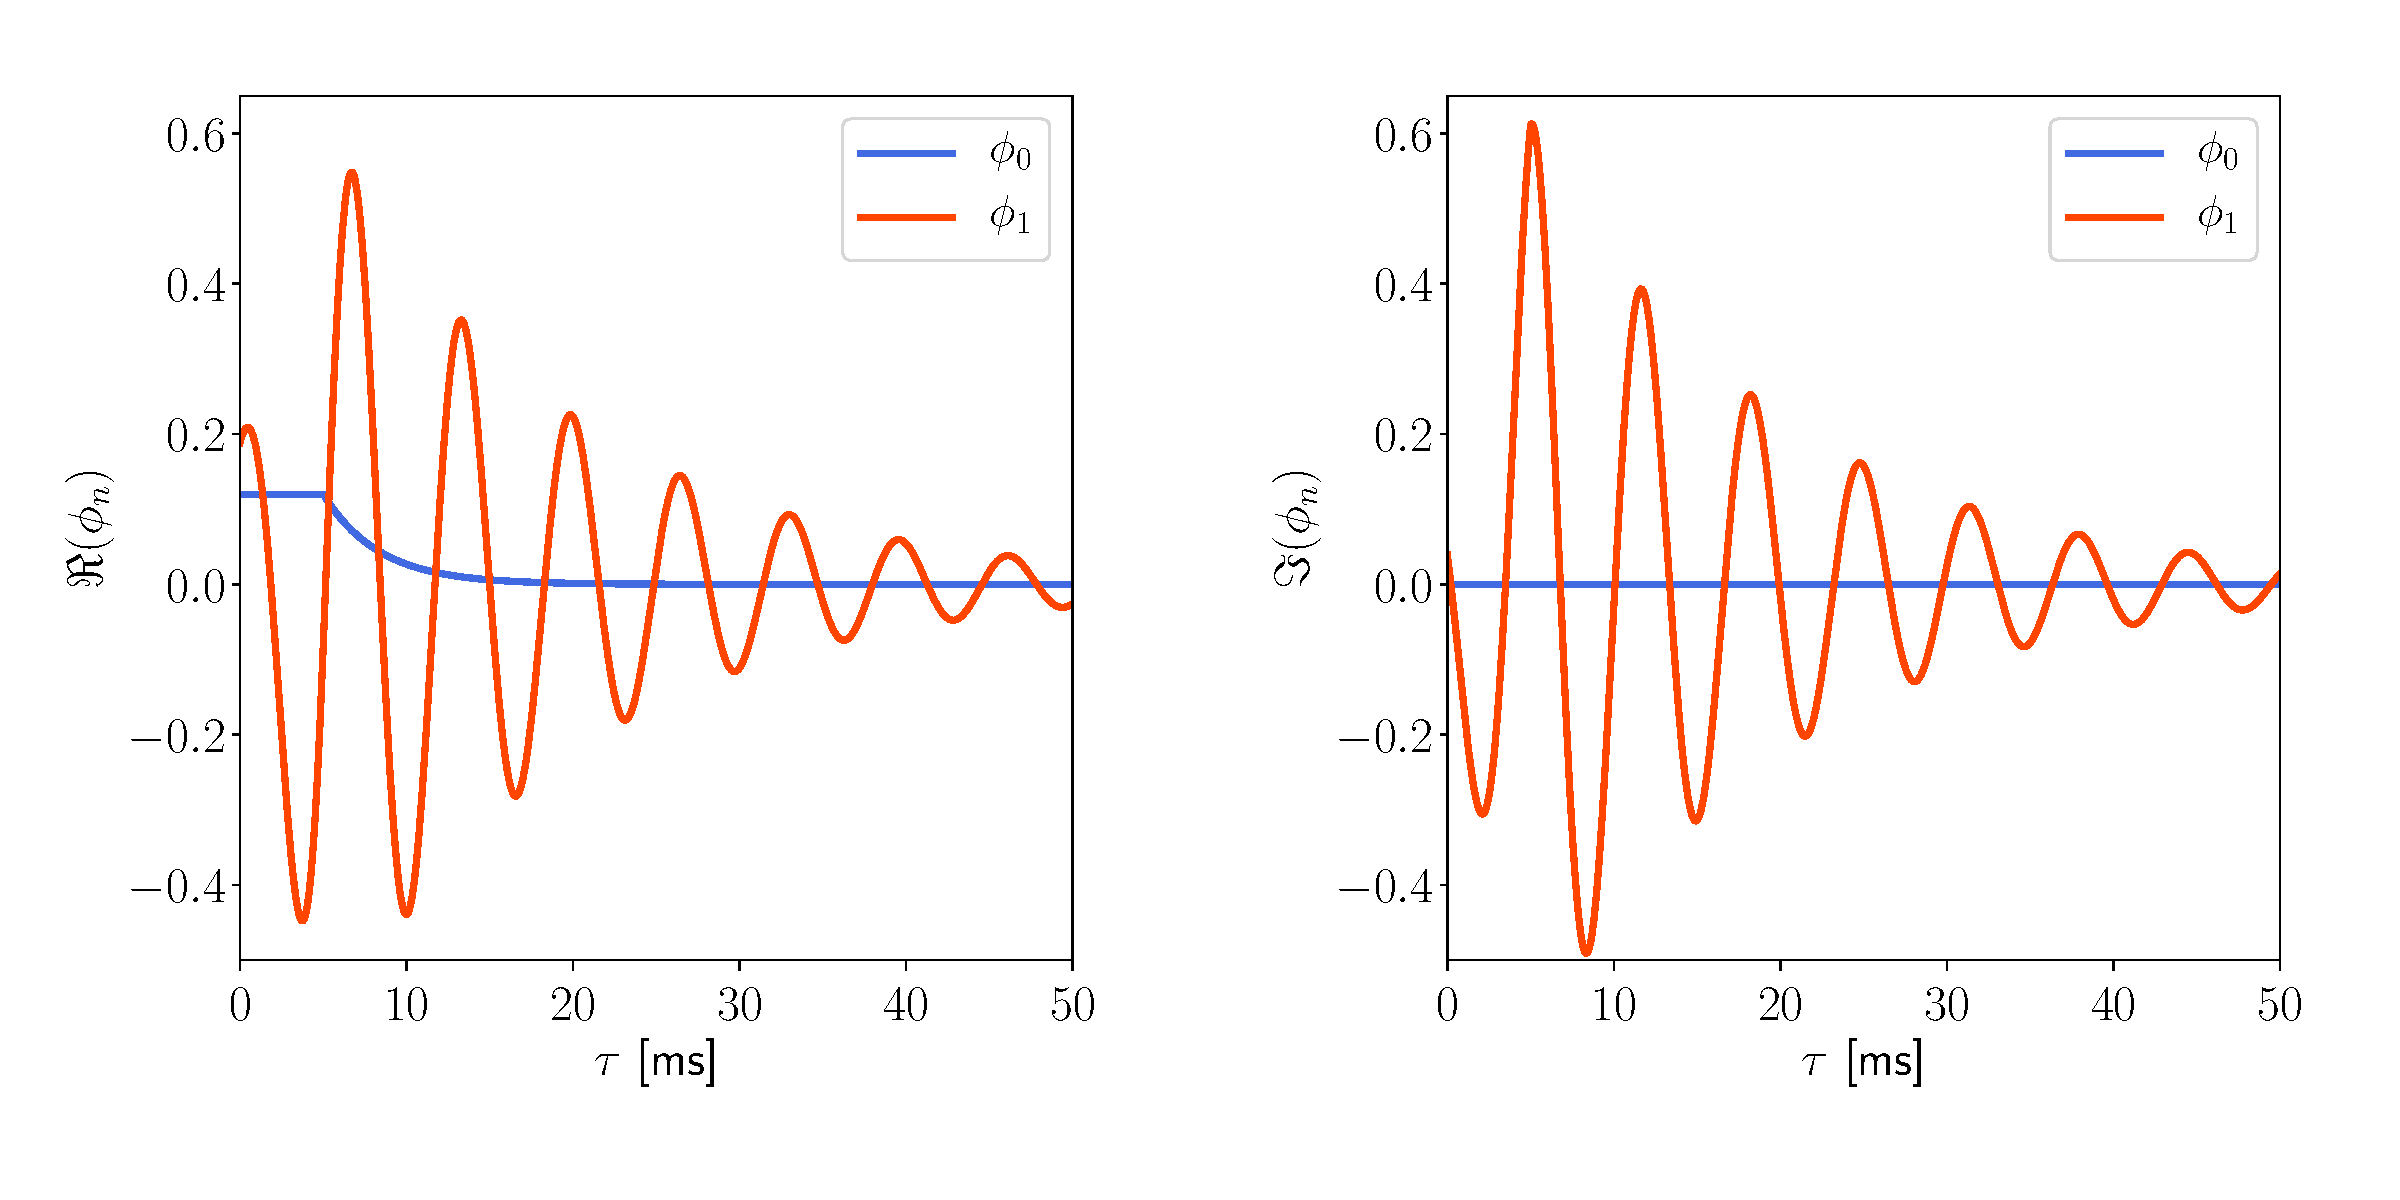
\includegraphics[width=0.8\linewidth]{poisson_eigenfunction2.pdf}
	\caption{Real part (left) and imaginary part (right) of the eigenfunctions $\phi_n$ of the first modes $n=0,1$ for a \textbf{Poisson neuron with absolute refractory period} $\Delta$. With $\Delta=5$ ms, $h=h_0$, $\nu_{max}=0.6$ kHz. $\phi_{-1}$ is the complex conjugate of $\phi_{1}$}
	\label{fig:poissoneigenfunction}
\end{figure} 

In this section we consider a Poisson neuron with absolute refractory period $\Delta$, the hazard rate is defined by the recovery function Eq.\eqref{eq:poissonabs}. For the sake of simplicity in the notation we will use the variable $\nu$ such that $\nu=\Phi(h)$. The hazard rate is then given by

\begin{equation}
\rho(\tau,h)=\nu\:\Theta(\tau-\Delta)
\end{equation}

And the interspike interval distribution is 
\begin{equation}
P(\tau,h)=\nu\exp\big(-\nu(\tau-\Delta)\big) \Theta(\tau-\Delta) 
\end{equation}


%\be
%S(\tau)=\Theta(\Delta-\tau) +  \Theta(\tau-\Delta) \exp(-\nu(\tau-\Delta))
%\ee
For this process we can compute the Laplace transform of the ISI density

\begin{align}
P_L(\lambda)=&\int_0^\infty P(\tau)e^{-\lambda \tau}\dd \tau\nonumber\\
=&\frac{\nu}{\nu+\lambda}\exp(-\lambda \Delta)
\end{align}
%=&\int_\Delta^\infty \nu \exp\big(-(\lambda+\nu)\tau)\big)\exp\big(\nu \Delta\big)\\


By the change of variable $w_n=(\nu+\lambda_n)\Delta$, the normalization condition Eq.\eqref{eq:condition2} $P_L(\lambda))=1$, can be rewritten as

%\frac{\nu}{\nu+\lambda}exp(-\lambda_n \Delta)=1

\begin{equation}
\label{eq:weq}
\Delta \nu e^{\nu\Delta}=w_ne^{w_n} 
\end{equation}

The solution of equation Eq.\eqref{eq:weq} is given introducing the Lambert W-function $W(z,n)$
\begin{equation}
w_n=W(\Delta \nu e^{\nu\Delta},n)
\end{equation}

from which we read the eigenvalue spectrum $\{\lambda_n\}$

\begin{equation}
\lambda_n=\frac{1}{\Delta}W(\Delta \nu e^{\nu\Delta},n) - \nu
\end{equation}

We can explicitly express the eigenfunctions, $\ket{\phi_n}$ of the operator $\mathcal{L}$ and $\ket{\psi_n}$ of  the adjoint operator $\mathcal{L}^+$

%\begin{align}
%\phi_n(0) =&\frac{1}{\int_0^{\infty}\big[1-\int^\tau_0 \nu \Theta(x-\Delta) \exp(-\nu(x-\Delta)) \exp\big(-\lambda_nx)dx\big]d\tau}\\
%=& \frac{\nu+\lambda_n}{1+\Delta(\nu+\lambda_n)}
%\end{align}

\begin{equation}
\phi_n(\tau)= \frac{\nu+\lambda_n}{1+\Delta(\nu+\lambda_n)}e^{-\lambda_n\tau}\left[\Theta(\Delta-\tau) +  \Theta(\tau-\Delta)e^{-\nu(\tau-\Delta)}\right]
\end{equation}

These eigenfunctions are illustrated in Fig.\ref{fig:poissoneigenfunction} for $n=0,1$

\begin{align}
\psi_n(\tau)=&\Theta(\Delta-\tau)e^{\lambda_n\tau} +  \Theta(\tau-\Delta) \frac{\nu}{\nu+\lambda_n}\nonumber\\
=&\Theta(\Delta-\tau)e^{\lambda_n\tau} +  \Theta(\tau-\Delta)e^{\lambda_n\Delta}
\end{align}\\

One can verify that the set ofeigenfunctions satisfy Eq.\eqref{eq:dij}.
So far we considered constant $h$. For the general case of time-dependent input, we need we need to compute $\frac{d\psi_n(\tau)}{d\nu}$, to define the coupling coefficients Eq.\eqref{eq:couplingcoef}. 

\begin{equation}
\frac{\partial\psi_n(\tau)}{\partial\nu}=\frac{\lambda_n}{\nu[1+\Delta(\nu+\lambda_n)]}\left[\Theta(\Delta-\tau)\tau e^{\lambda_n\tau} +  \Theta(\tau-\Delta)\Delta e^{\lambda_n\Delta}\right]\\
\end{equation}\\

The coupling coefficients are then given by
\begin{align}
C_{nn}=&\frac{\partial \nu}{\partial h}\int_0^\infty\frac{d\psi_n(\tau)}{d\nu}\phi_n(\tau)d\tau \nonumber\\
=&\frac{\lambda_n\Delta(1+\frac{1}{2}\lambda_n(\nu+\lambda_n))}{\nu(1+\Delta(\nu+\lambda_n))}\frac{\partial \nu}{\partial h}
\end{align}


\begin{align}
C_{nm}=&\frac{\partial \nu}{\partial h}\int_0^\infty\frac{d\psi_n(\tau)}{d\nu}\phi_m(\tau)d\tau \nonumber\\
=&\frac{\lambda_n(\nu+\lambda_m)}{\nu(\lambda_n-\lambda_m)(\nu+\lambda_n)(1+\Delta(\nu+\lambda_m))}\frac{\partial \nu}{\partial h}
\end{align}




\subsection{Gamma neuron model}

\begin{figure}[h!]
	\centering
	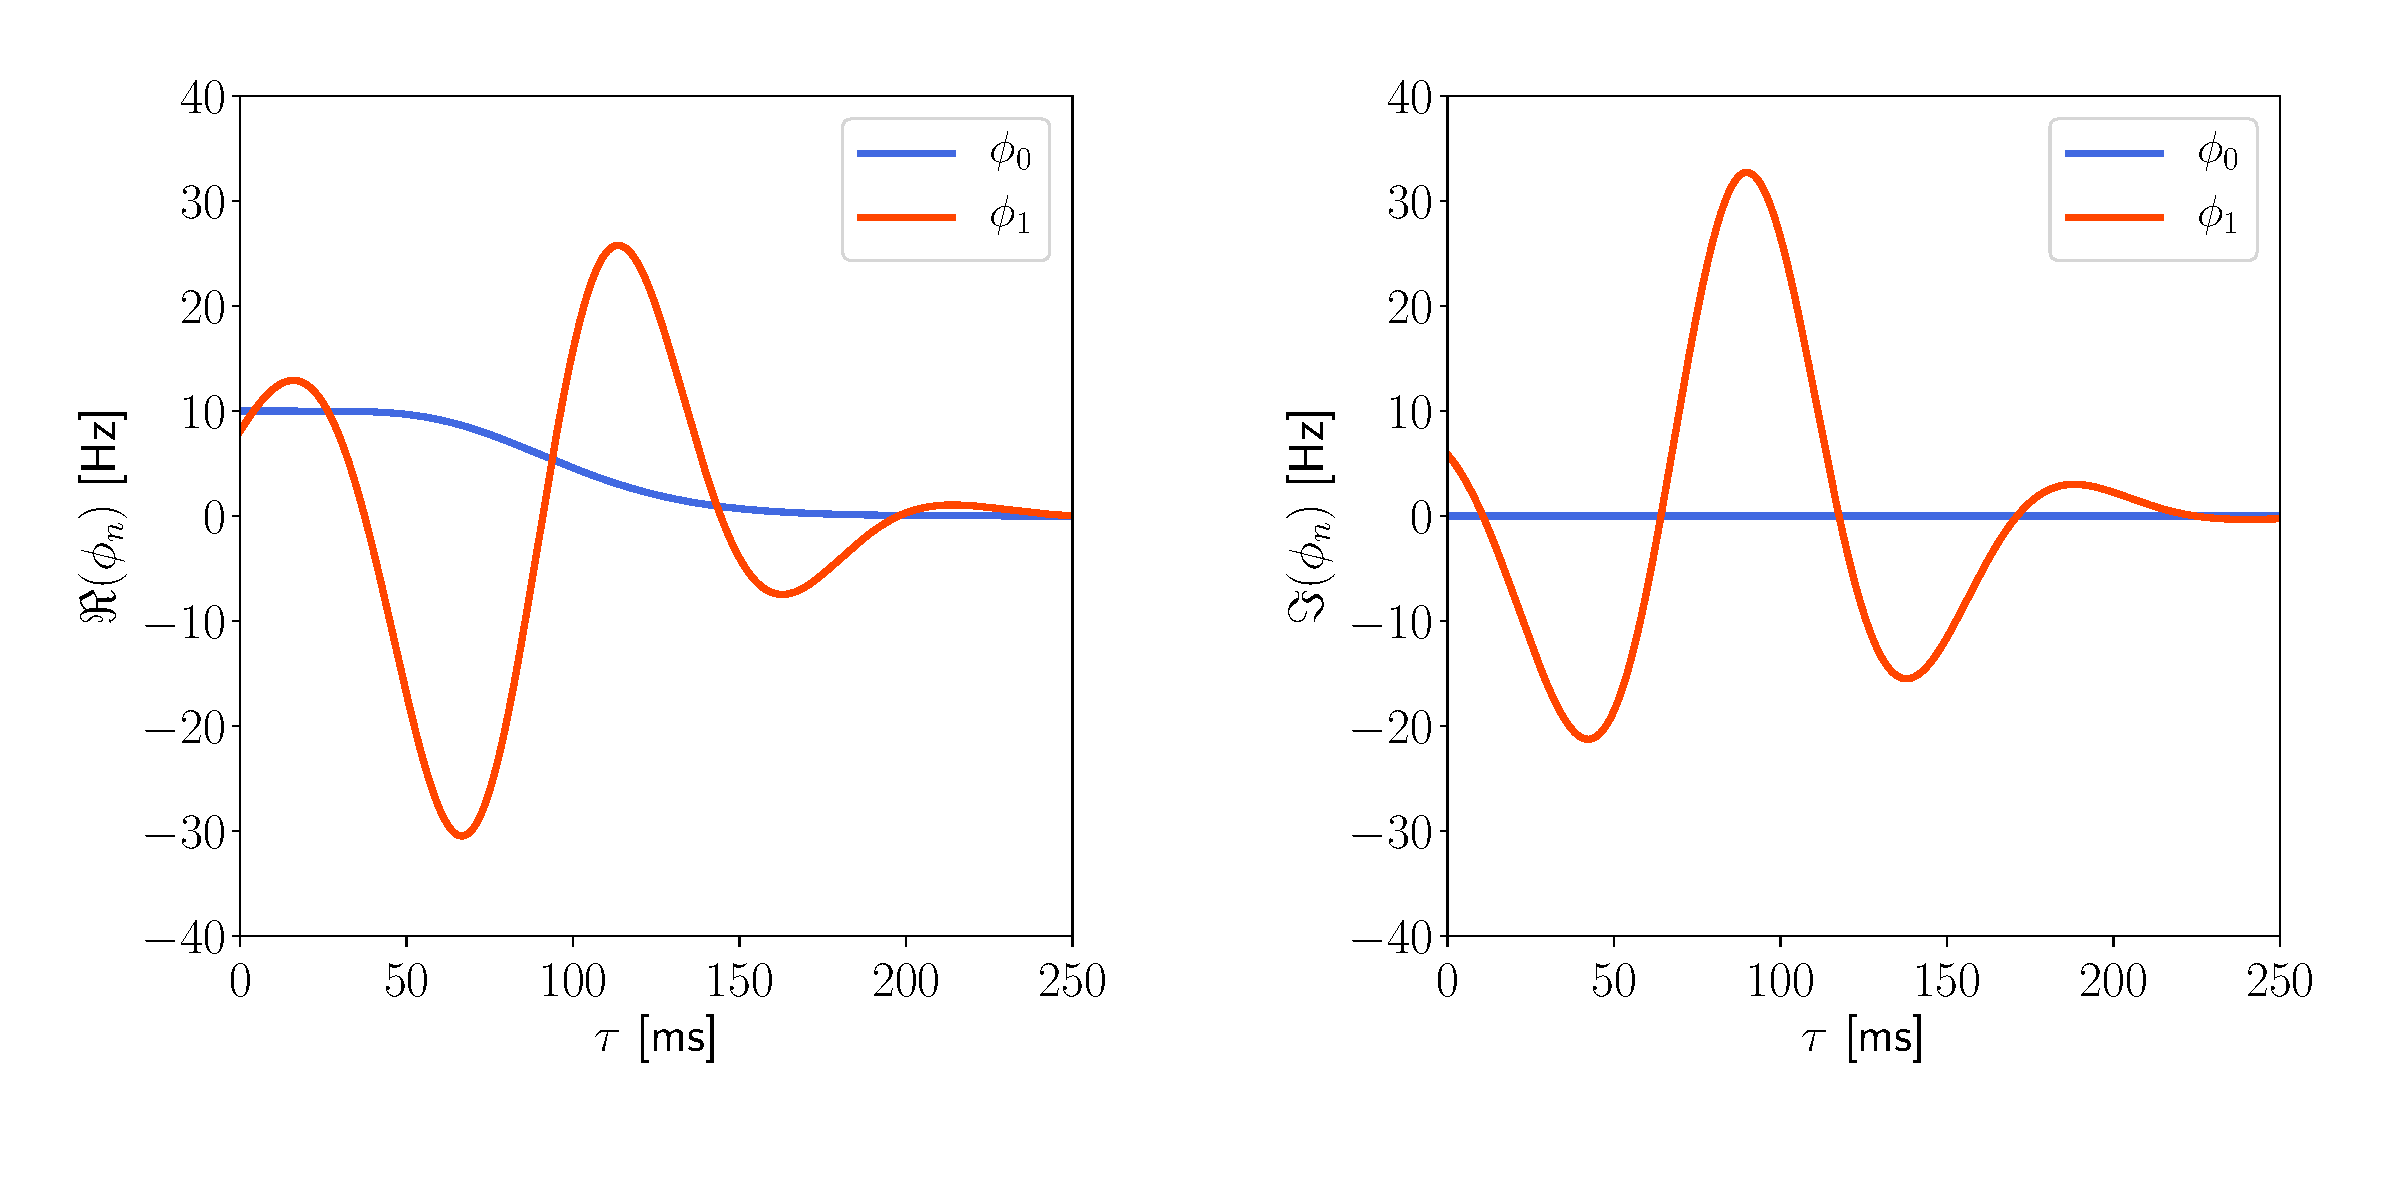
\includegraphics[width=0.8\linewidth]{gamma_eigenfunction.pdf}
	\caption{Real part (left) and imaginary part (right) of the eigenfunction $\phi_n$ of the first modes for a \textbf{Gamma neuron model} with $\beta=100$
		$\gamma=10$. $\phi_{-1}$ is the complex conjugate of  $\phi_{1}$}
	\label{fig:gammaeigenfunction}
\end{figure}

In this section we consider a gamma neuron model. Taking the Laplace transform of the ISI density Eq.\eqref{eq:gamma} yields

\begin{equation}
P_L(\lambda)=\left(\frac{\beta}{\beta +\lambda}\right)^\gamma
\end{equation}

The condition given by Eq.\eqref{eq:condition2} leads then to the solutions [\cite{Sch16}]

\begin{equation}
\label{eq:gammaeig}
\lambda_n=\beta\left(\exp\left(\frac{2\pi i}{\gamma}n\right)-1\right), \hspace{2.8cm}  n=0,..., \gamma-1
\end{equation}

Interestingly the gamma neuron model has a finite number of mode. Eq.\eqref{eq:gammaeig} can be rewritten in function of the rate $R$ and the coefficient of variation $C_V$ as

\begin{equation}
\lambda_n=RC_V^{-2}\left(\exp\left(2\pi iC_V^2 n\right)-1\right)
\end{equation}

And the normalization Eq.\eqref{eq:psi0} yields to
\begin{equation}
\phi_n(0)=\frac{1}{\gamma\beta^\gamma(\beta+\lambda_n)^{-(\gamma+1)}}
\end{equation}

The eigenfunctions of the gamma  neuron model are illustrated in Fig.\ref{fig:gammaeigenfunction} for $n=0,1$.


\subsection{PIF model}

In this section we will consider the perfect integrating and fire neuron modem. The Laplace transform of the ISI density Eq.\eqref{eq:inversegaussian} is

\begin{equation}
P_L(\lambda)=\exp\big(\frac{f(h) V_{th}\tau_v}{2D}\big[1-\sqrt{1+\frac{4D\lambda}{f(h)^2}}\big]\big)
\end{equation}


The condition given by Eq.\eqref{eq:condition2} leads then to the solutions
\begin{equation}
\lambda_n=-\frac{4\pi D}{\tau_V^2V_{th}^2}n^2+\frac{f(h)}{V_{th}\tau_v}ni
\end{equation}

The spectrum can be rewritten as a function of the rate $R$ and the coefficient of variation $C_V$

\begin{equation}
\lambda_n=- 2\pi^2RC_V^2n^2+2\pi R i\:n
\end{equation}

We could not find an analytical solution for the normalization equation Eq.\eqref{eq:normalization}.

\section{A general approximation of the spectrum}
\label{sec:eigv}
In the previous sections we derived the spectrum $\{\lambda_n\}$ for different specific neuron models. But for a general ISI distribution $P(\tau)$, it is not always possible to obtained a analytical form of the Laplace transform $P_L(\lambda)$. Thats why we would like to find a method to approximate the first eigenvalue $\lambda_1$. From Eq.\eqref{eq:Pmoment2} one can see that the the Laplace transform of the ISI distribution can be rewritten with the cumulant $\kappa_n$ as

\begin{equation}
\label{eq:PLcum}
P_L(\lambda)=\exp\left[ \sum_{k=1}^{+\infty}(-1)^k\kappa_k \frac{\lambda^k}{k!}\right]
\end{equation}

The condition $P_L(\lambda_n)=1=\exp(2\pi \i n)$ Eq.\eqref{eq:condition2} can be rewritten as


\begin{equation}
\label{eq:cum2pi}
\sum_{k=1}^{+\infty}(-1)^k\kappa_n \frac{\lambda_n^k}{k!}=2 \pi i n
\end{equation}

We can approximate the first eigenvalue $\lambda_1$, neglecting the terms multiplied by the cumulants $\kappa_k$ for $k>2$. Consequently Eq.\eqref{eq:cum2pi} becomes

\begin{equation}
\label{eq:cumaprox}
\frac{\kappa_2}{2}\lambda_1^2-\kappa_1\lambda_1 -2\pi i=0
\end{equation}

$\lambda_1$ correspond to the roots of Eq.\eqref{eq:cumaprox} with the negative real parts, as we have shown before in Section \ref{sec:op}, a positive real part would be unphysical and does not satisfy Eq.\eqref{eq:condition2}. The approximation of $\lambda_1$ can be rewritten in terms of the rate $R$ and the coefficient of variation $C_V$ using Eq.\eqref{eq:R} and Eq.\eqref{eq:CV}

\begin{equation}
\label{eq:l1aprox}
\lambda_1\simeq RC_V^{-2}\left( 1-\sqrt{1+4\pi i C_V^2}\right)
\end{equation}

\begin{figure}[h!]
	\centering
	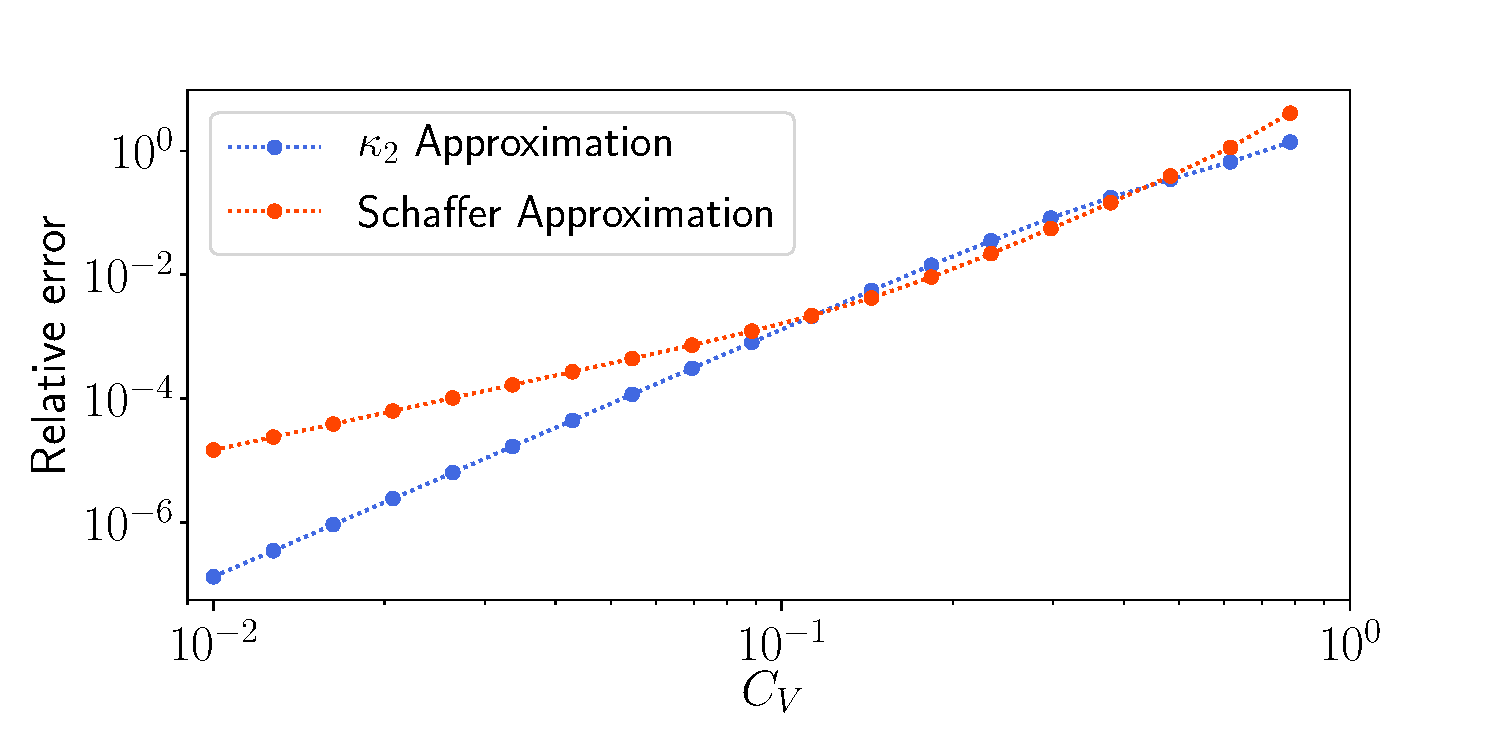
\includegraphics[width=0.8\linewidth]{kumulant_gamma.pdf}
	\centering
	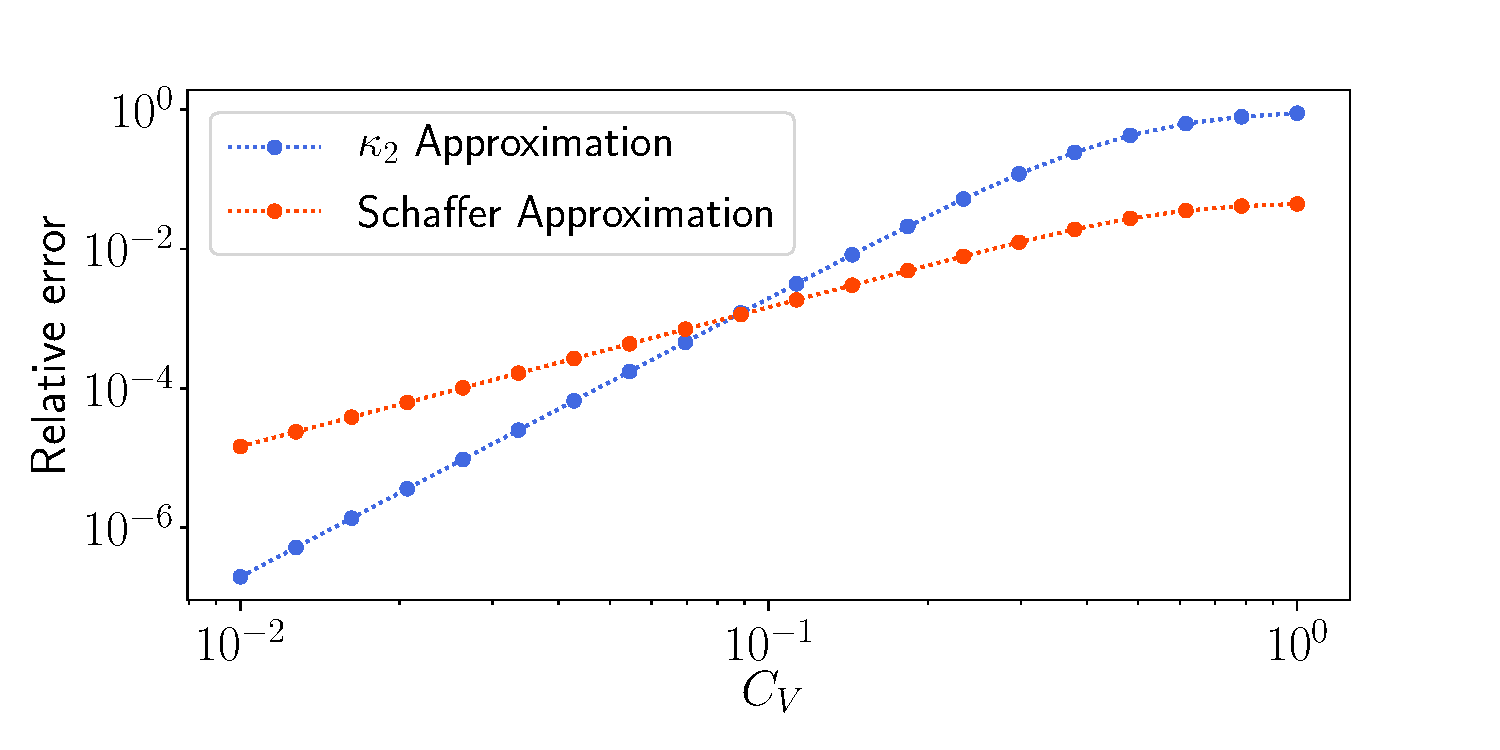
\includegraphics[width=0.8\linewidth]{kumulant_pif.pdf}
	\caption{\textbf{Top:} Gamma  neuron model. \textbf{Bottom:} PIF neuron modle. Relative error on the eigenvalue for the eigenvalue approximations derived by \cite{SchOst13} Eq.\eqref{eq:schaffer}, and by Eq.\eqref{eq:l1aprox} using the cumulant expansion as a function of $C_V$.}
	\label{fig:kumulant}
\end{figure}


In \cite{SchOst13},  they determined the first eigenvalue $\lambda_1$ for different renewal processes by fitting the dependency of the real part and the imaginary part on the rate $R$ and on the coefficient of variation squared $C_V^2$. They found as a relationship for small $C_V$:

\begin{equation}
\label{eq:schaffer}
\lambda_1 \simeq -R\left( \left(\frac{C_V}{0.22}\right)^2+2\pi i\right) 
\end{equation}

Note that for small $C_V$ we can Taylor expand the square root in Eq.\eqref{eq:l1aprox} and recover an expression close to Eq.\eqref{eq:schaffer}

\begin{equation}
\label{eq:l1aprox2}
\lambda_1\simeq -R\left(2\pi^2 C_V^2+2\pi i\right) + \mathcal{O}(C_V^4)
\end{equation}

Indeed $\frac{1}{(0.22)^2}\simeq20.7$ and $2\pi^2\simeq19.7$.

Fig.\ref{fig:kumulant} shows the relative error $\frac{|\lambda_1 -\hat{\lambda}_1|}{|\lambda_1|}$ for the different approximation $\hat{\lambda}_1$ of the first eigenvalue $\lambda_1$. 

For the Gamma neuron model the relative error is below $0.1$ for $C_V<0.3$ for the approximation obtained by Schaffer et al Eq.\eqref{eq:schaffer} and the one given by Eq.\eqref{eq:l1aprox}. For $C_V<0.1$ Eq.\eqref{eq:l1aprox} is a better approximation. 

For the PIF neuron model, the $\kappa_2$ approximation has a relative error below $0.1$ for $C_V<0.1$. It becomes better than the Schaffer approximation for $C_V<0.1$. Actually Eq.\eqref{eq:l1aprox2} is exact thus for small $C_V$, the relative error with the $\kappa_2$ is very low and we saw that the Schaffer approximation is close to this expression, so even for large $C_V$ the Schaffer approximation is good.

 It seems that the truncation of the cumulant sum to second order gives a good approximation of the first eigenvalue $\lambda_1$ for small $C_V$.  %Those preliminary results must be further investigated.

\chapter{Evaluation of spectral approximations}
\label{chap:grene}

\section{Transcient response of the population activity starting with a delta distribution $q(\tau,0)=\delta(\tau)$}

\begin{figure}[h!]
	\centering
	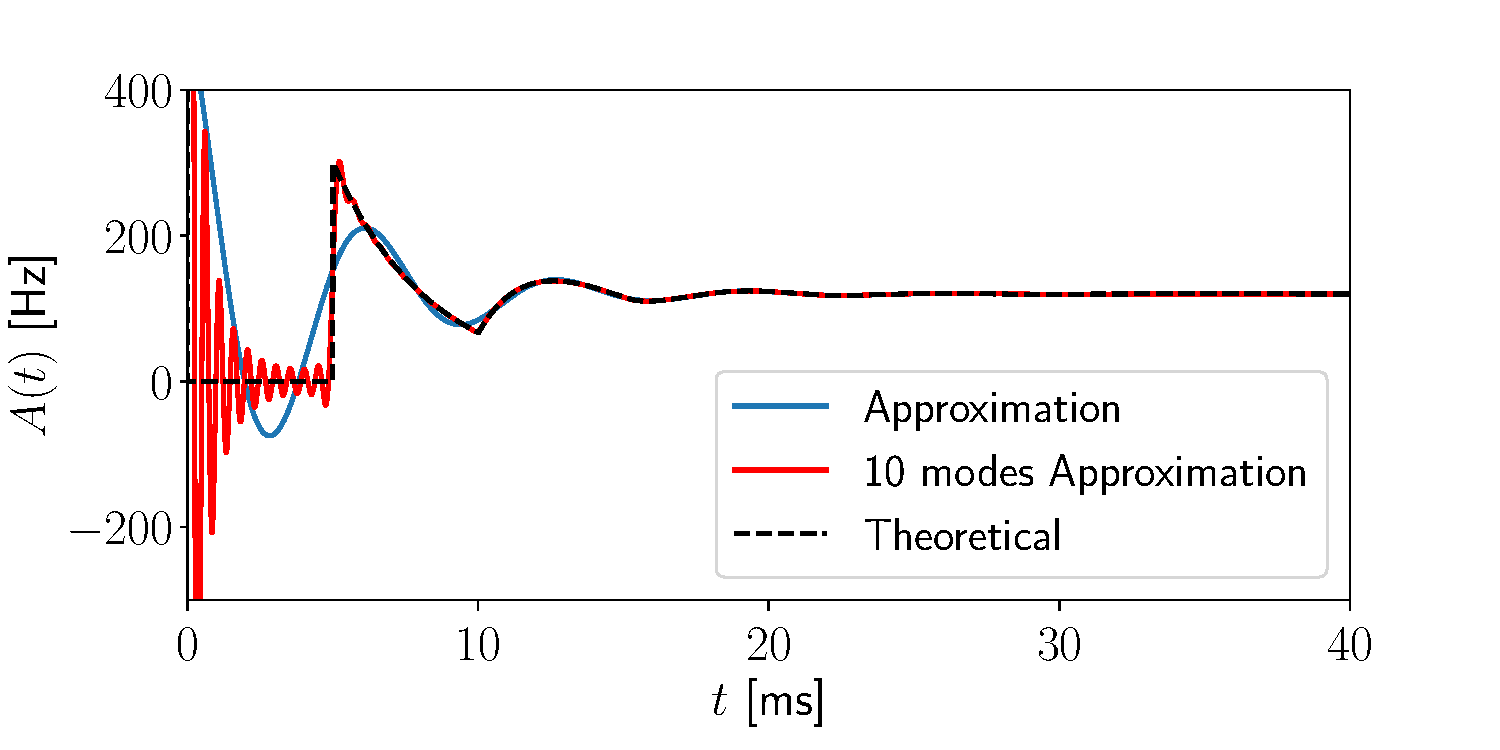
\includegraphics[width=0.8\linewidth]{delta_poisson.pdf}
	\caption{Activity $A(t)$ of a population of neuron of poisson neuron with absolute refractoriness $\Delta$ The approximation given by Eq.\eqref{eq:A3}, and the 10 modes approximation is given by  by Eq.\eqref{eq:A2} with $n=10$. The parameters used are $h=h_0$, $\Delta=5$ ms, and $\nu_{max}=0.6$ $kHz$  and the initial condition is $q(\tau,0)=\delta(\tau)$}
	\label{fig:delta_poisson}
\end{figure}

In this section we will look at the result of the approximation Eq.\eqref{eq:A4} for the gamma  neuron model and for a population of Poisson neurons with absolute refractoriness. For the sake of simplicity we consider first a large homogeneous population of uncoupled neurons with a constant input potential.The initial distribution of the refractory density $q$ is given by a delta peak $q(\tau,0)=\delta(\tau$), i.e all neurons spike at time $t=0$.

As expected for the Poisson neuron with absolute refractoryness model, we need infinitely many modes to recover the exact initial distribution Fig.\ref{fig:delta_poisson}. We will see later that keeping only the first mode is a good approximation for changes that are not too fast, which is not the case of a delta peak. Nevertheless  Fig.\ref{fig:delta_poisson} one can see that we quantitatively reproduce the response i.e the oscillations of the activity with the approximation given by Eq.\eqref{eq:A4}, and we even recover the shape of the first peak taking the $10$ first mode of Eq.\eqref{eq:A2}.

The Gamma neuron model has a finite number of modes Eq.\eqref{eq:gammaeig} and we see on Fig.\ref{fig:delta_poisson} that we recover exactly the activity $A(t)$ taking the complete expansion.

\begin{figure}[h!]
	\centering
	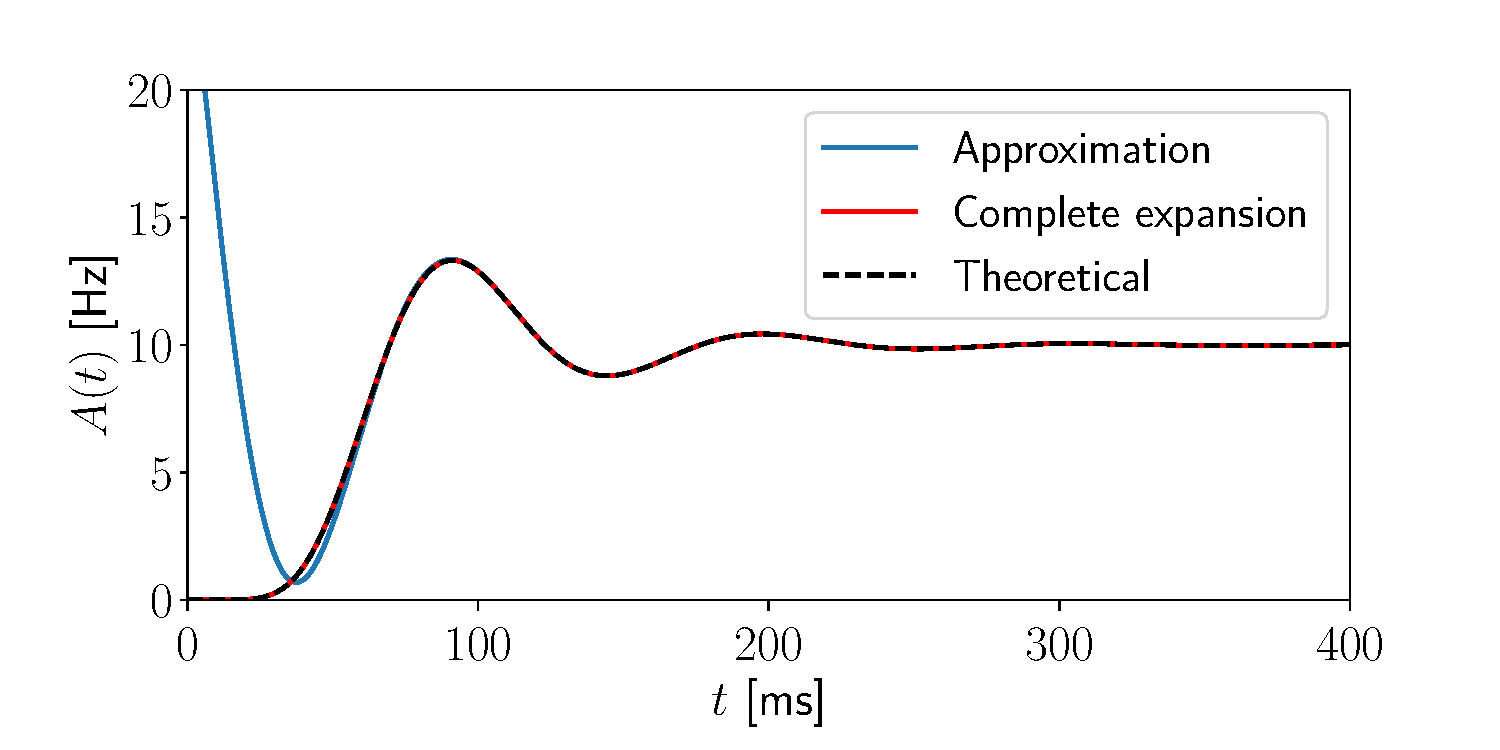
\includegraphics[width=0.8\linewidth]{delta_gamma.pdf}
	\caption{Activity $A(t)$ of a population of neurons having an ISI density given by the gamma distribution with $\beta=100$ Hz and $\gamma=10$ starting with a delta distribution $q(\tau,0)=\delta(\tau)$. With the approximation given by Eq.\eqref{eq:A4}, and the complete expansion given by Eq.\eqref{eq:A2}}
	\label{fig:delta_gamma}
\end{figure}


\section{Population response to time-dependent input}
\label{sec:uncoupletimedep}

\begin{figure}[h!]
	\centering
	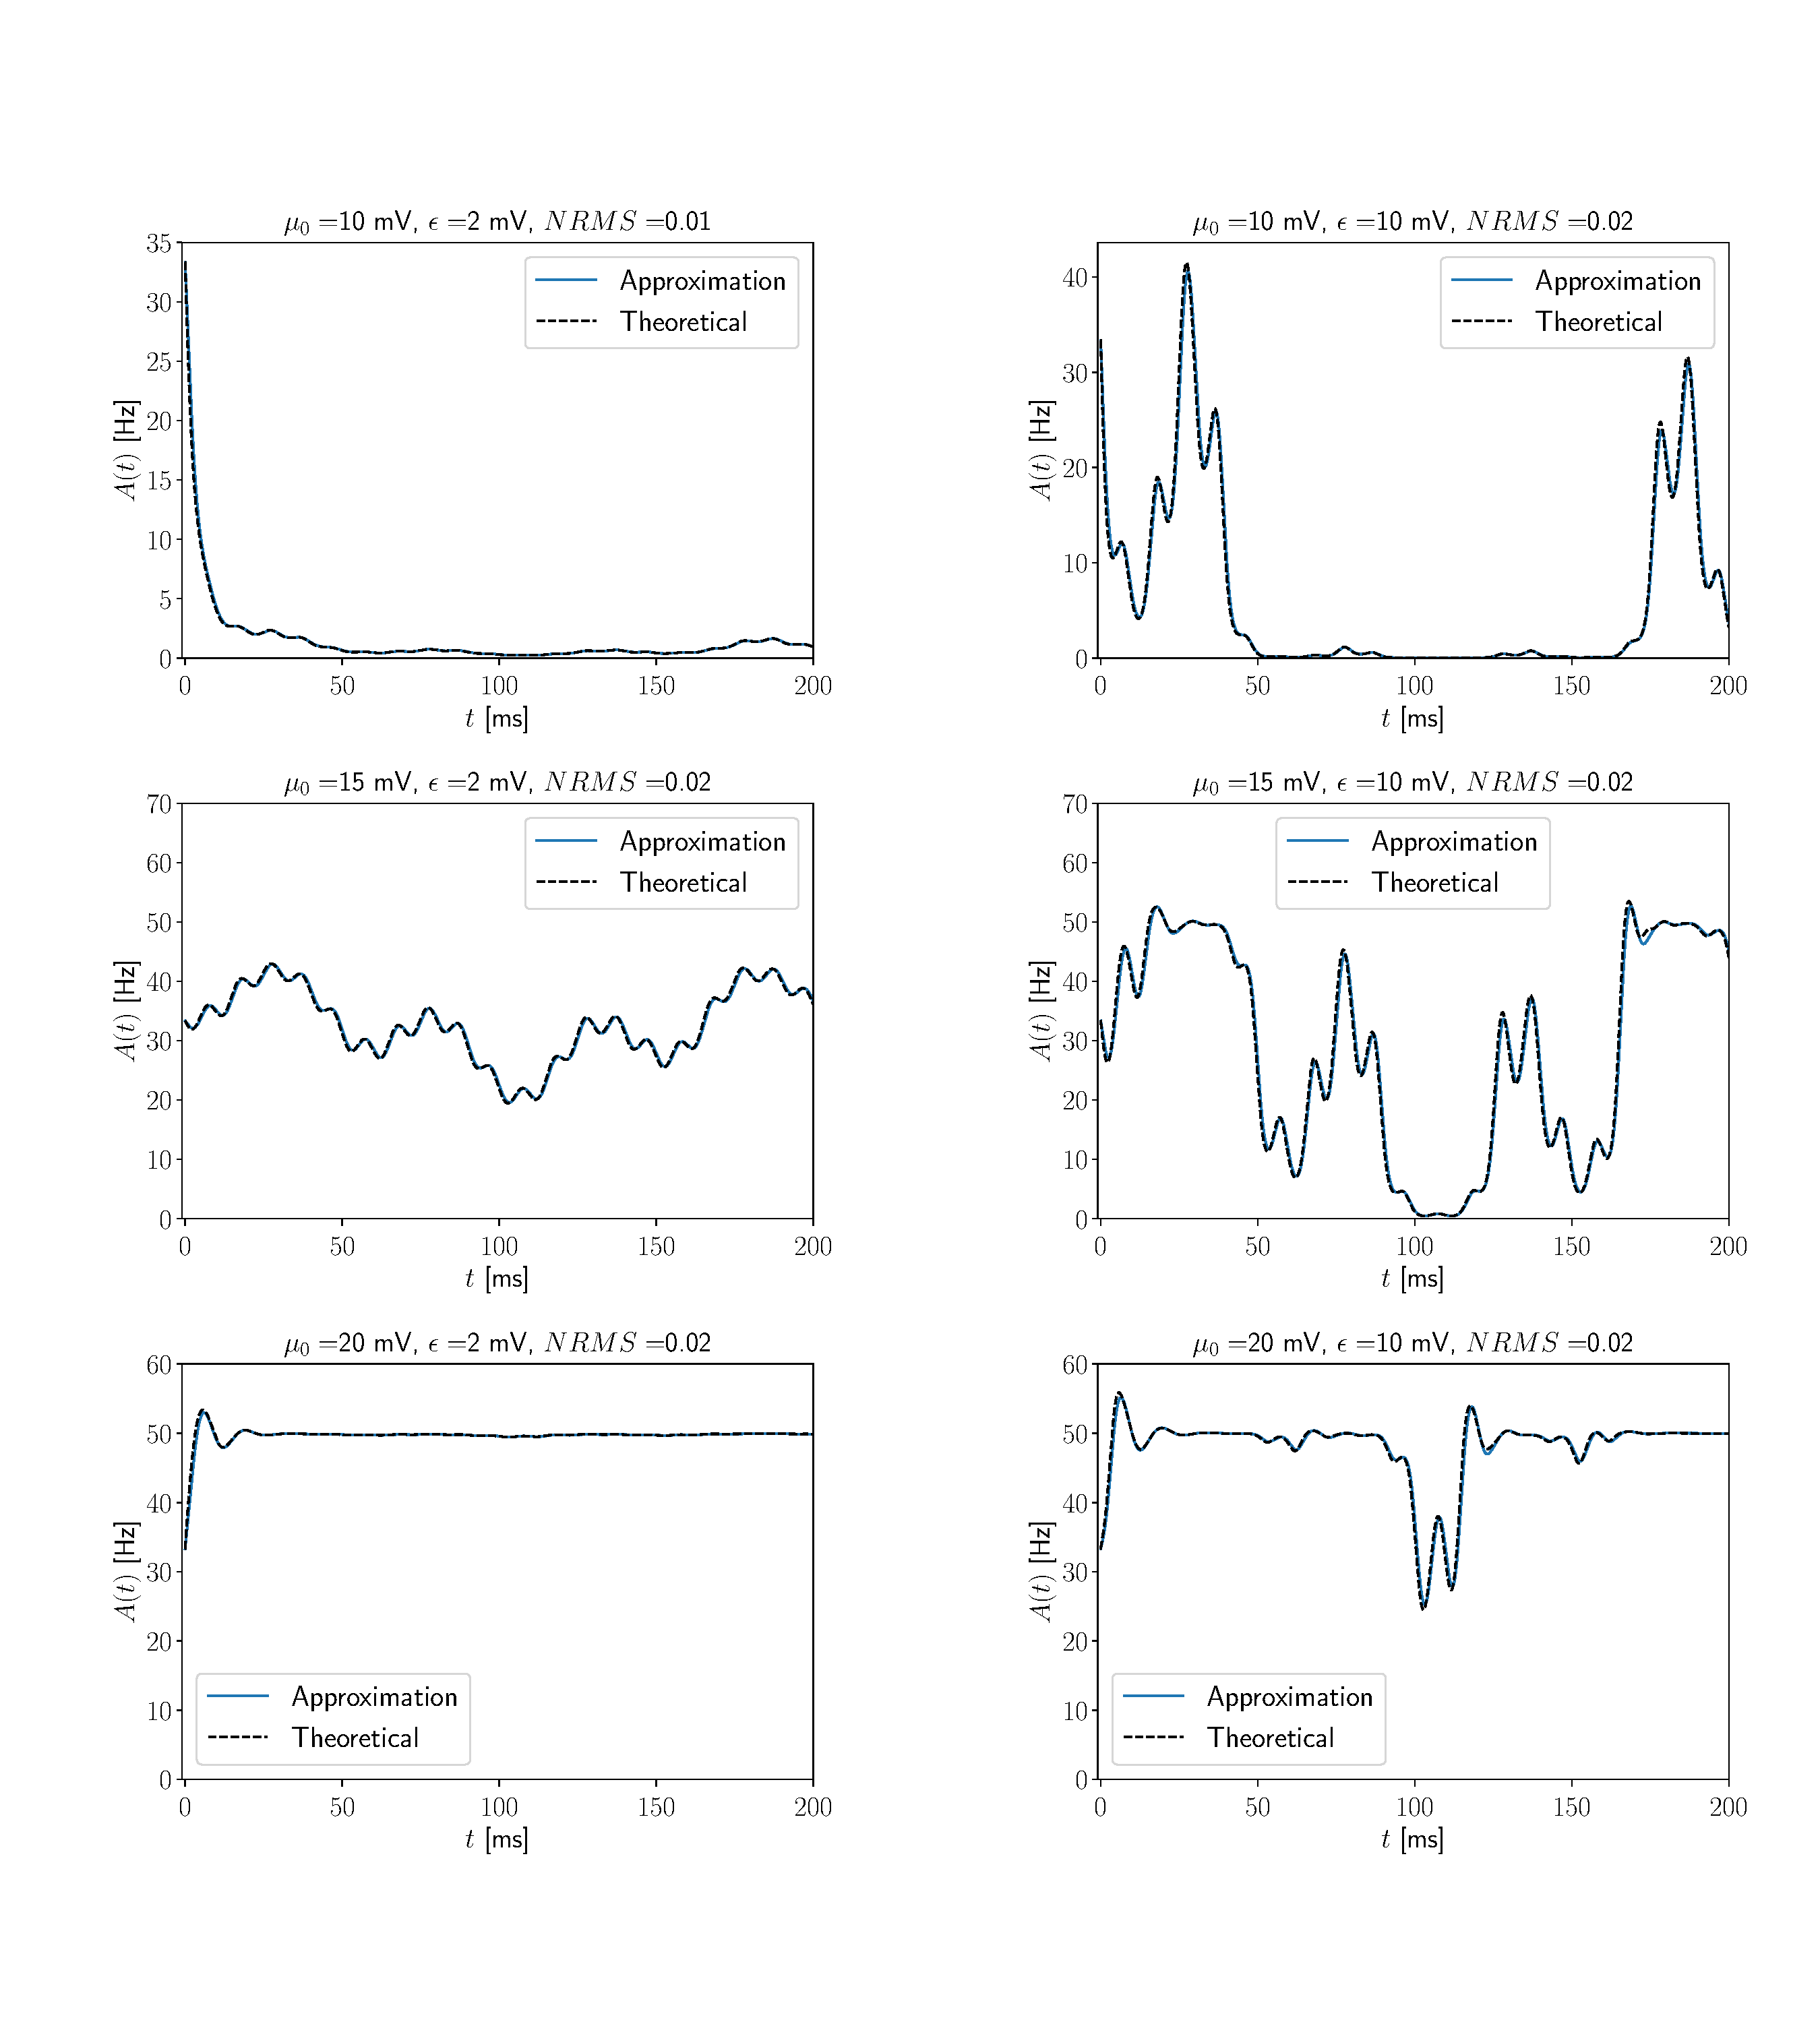
\includegraphics[width=0.9\linewidth]{A_t.pdf}
	\caption{Response of a population of uncoupled Poisson neurons with absolute refractoriness to a fluctuating external input given by Eq.\eqref{eq:mu2}. For different amplitude $\epsilon$ of the oscillating function $f_{cos}(t)$(left: $\epsilon=2$ mV, right: $\epsilon=10$ mV)), for different baseline of the external potential input, top: $\mu_0 < h_0$, middle  $\mu_0 = h_0$ and bottom: $\mu_0 > h_0$ The parameters of the neurons are $\nu_{max}=100$ Hz, $\Delta=10$ ms, $\beta=1$ mV$^{-1}$ , $h_0=15$ mV. The time constant of the input potential $h$ is $\tau_m=10$ ms.
	}
	\label{fig:A_t}
\end{figure}


\begin{figure}[h!]
	\centering
	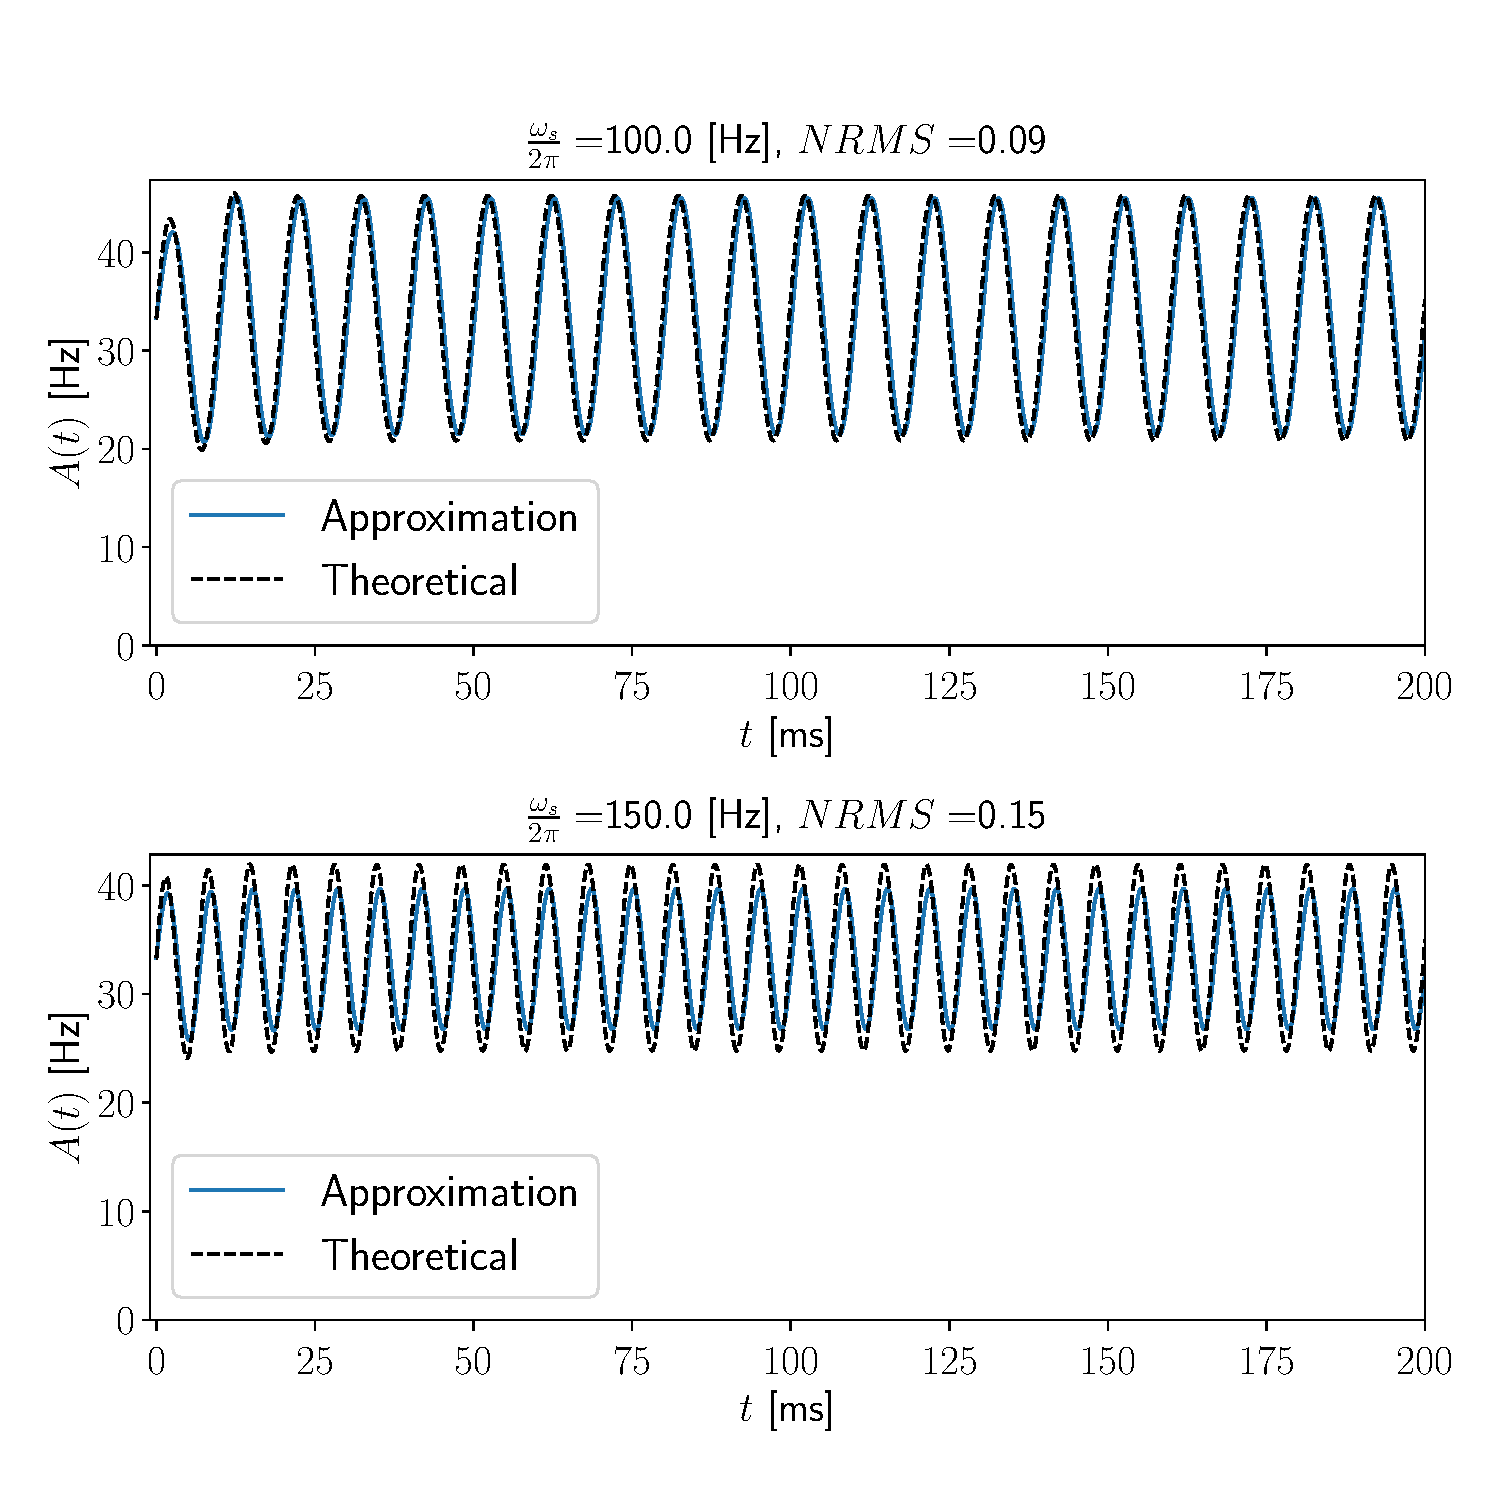
\includegraphics[width=0.8\linewidth]{A_omega_t.pdf}
	\caption{Population response to an oscillating input $\mu(t)$ with angular frequency $\omega_s$ (top: $100$ Hz, bottom $150$ Hz ), for a large populations of uncoupled Poisson neurons with absolute refractoriness. The parameters of the neurons are $\nu_{max}=100$ Hz, $\Delta=10$ ms, $\beta=1$ mV$^{-1}$ , $h_0=15$ mV. The time constant of the input potential $h$ is $\tau_m=10$ ms.
	}
	\label{fig:A_omega_t}
\end{figure}


\begin{figure}[h!]
	\centering
	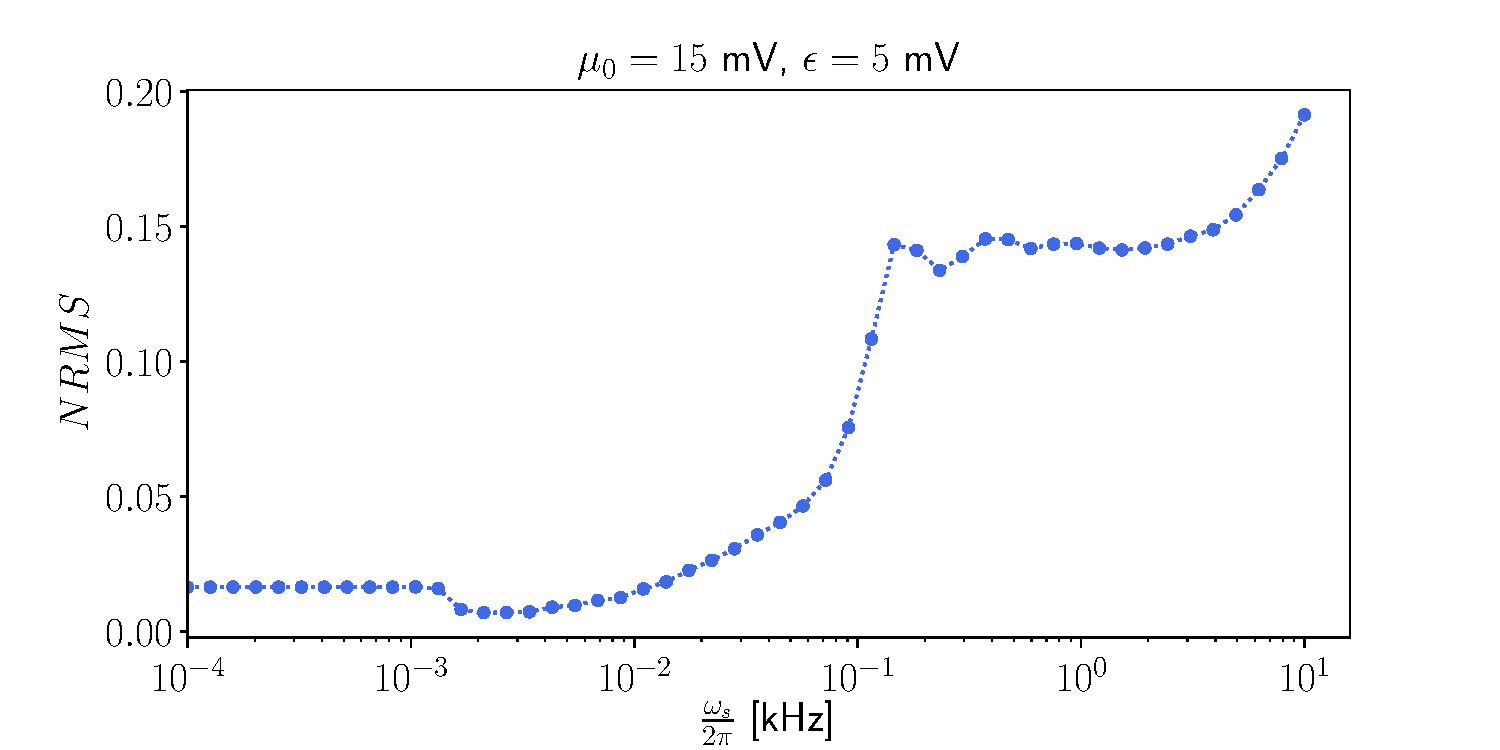
\includegraphics[width=0.8\linewidth]{NRMSo.pdf}
	\caption{NRMS on the response of population of uncoupled Poisson neurons with absolute refractoriness as a function of the angular frequency $\omega_s$  of the sinusoidal modulation of the external input potential $\mu(t)$ Eq.\eqref{eq:mut}. The parameters of the neurons are $\nu_{max}=100$ Hz, $\Delta=10$ ms, $\beta=1$ mV$^{-1}$ , $h_0=15$ mV. The time constant of the input potential $h$ is $\tau_m=10$ ms.
	}
	\label{fig:NRMSo}
\end{figure}




\begin{figure}[h!]
	\centering
	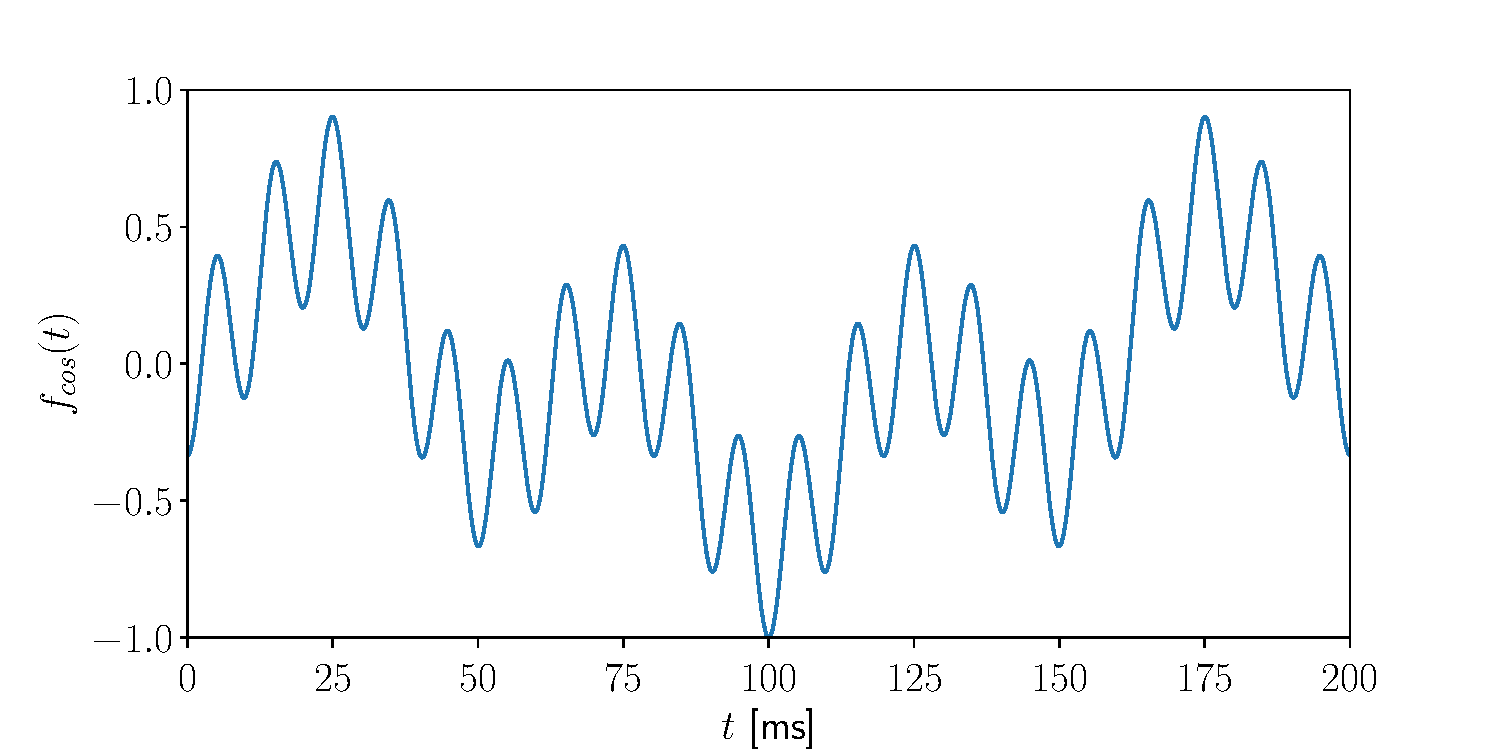
\includegraphics[width=0.8\linewidth]{fcos.pdf}
	\caption{Mix of equal amplitude sinusoidal oscillation with different frequencies: $5$, $20$ and $100$ Hz. $f_{cos}(t)=\frac{1}{3}\left(\cos(\omega_1t)-\cos(\omega_2t)-\cos(\omega_3t)\right)$
	}
	\label{fig:fcos}
\end{figure}


In this section we will study the response of a large population of uncoupled (i.e $J=0$) Poisson neuron with absolute refractoriness to an external time dependent input potential $\mu(t)$. The differential equation for the input potential $h$ is given by Eq.\eqref{eq:h}, and the firing rate of the Poisson neurons is given by $\Phi(h)$ Eq.\eqref{eq:phi}. We will compare the population activity approximation given by Eq.\eqref{eq:A4}, to the theoretical one computed as

\begin{equation}
A(t)=\Phi(h)\left(1-\int_{t-\Delta}^t A(s)\dd s\right)
\end{equation}

We will use as an error measure the normalized root-mean-square deviation NRMS.
The NRMS of predicted values $\hat {y}_t$ for times $t$ of a variable $y_t$ with variables observed over $T$ times, is computed as the square root of the mean of the squares of the deviations normalized by the range of value of $y$

\begin{equation}
\label{eq:NRMS}
NRMS=\frac{1}{y_{max}-y_{min}}\sqrt{\frac{\sum_{t=1}^T(\hat{y}_t-y_t)^2}{T}}
\end{equation}

Our approximation Eq.\eqref{eq:A4} only keeps the slowest mode, so we expect that the theory breaks down for fast inputs. To study the accuracy of our approximation, we looked at the response of the model to a sinusoidal modulation of the external input potential $\mu(t)$ with an angular frequency $\omega_s$ 

\begin{equation}
\label{eq:mut}
\mu(t)=\mu_0 + \epsilon \cos(\omega_st)
\end{equation}

The input potential was initialized as if the population activity was at a stationary state with $h(0)=\mu_0=h_0$. 

The results are summarized in Fig.\ref{fig:NRMSo}. For frequencies higher than $100$ Hz, the NRMS becomes high thus the approximation does not hold anymore. On Fig.\ref{fig:A_omega_t}, one can see that for a frequency of $150$ Hz the activity amplitude of the approximation becomes lower than the theoretical one.

To study the population response to more complex signals we used as external input

\begin{equation}
\label{eq:mu2}
\mu(t)=\mu_0+\epsilon f_{cos}(t)
\end{equation} 


Where $\mu_0$ and $\epsilon$ are constant and $f_{cos}(t)$  is a function composed of equal-amplitude sinusoidal oscillation with different frequencies. $f_{cos}(t)$ is represented of Fig.\ref{fig:fcos}. Fig.\ref{fig:A_t} illustrates the response for different $\mu_0$ and $\epsilon$. In the sub threshold $\mu_0<<h_0$ the activity is shut down due the sigmoid rate function $\Phi(h)$. In the suprathreshold limit $\mu_0>>h_0$ the activity goes toward the value $\frac{\nu_{max}}{1+\Delta\nu_{max}}$. Fig.\ref{fig:NRMSe} illustrates the accuracy of the approximation for the different input. For the different input the NRMS stays below $2.5\%$ which highlight the validity of the approximation.

\begin{figure}[h!]
	\centering
	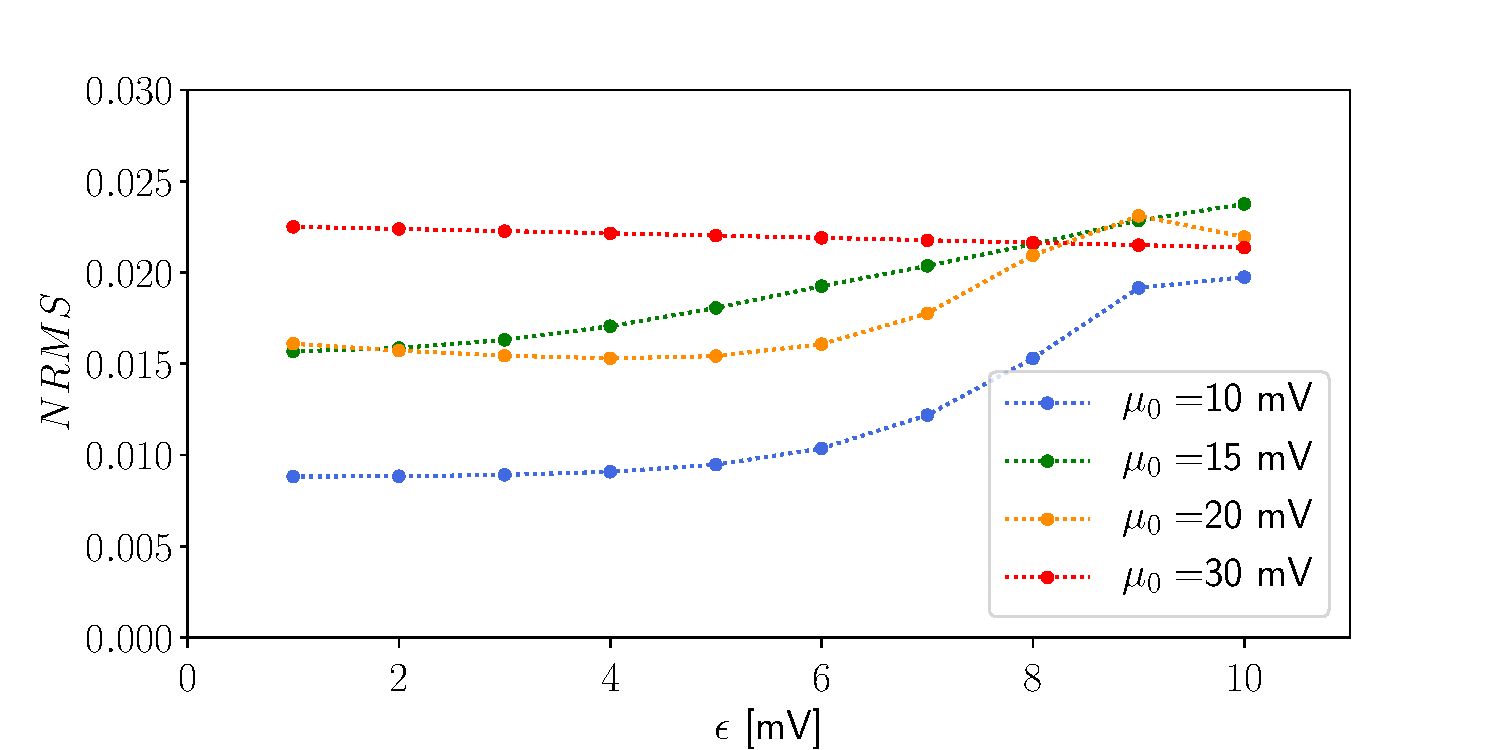
\includegraphics[width=0.8\linewidth]{NRMSe.pdf}
	\caption{NRMS on the response of population of uncoupled Poisson neurons with absolute refractoriness to a fluctuating external input given by Eq.\eqref{eq:mu2}. For different amplitude $\epsilon$ of the oscillating function $f_{cos}(t)$, for different baseline potential $\mu_0$. The parameters of the neurons are $\nu_{max}=100$ Hz, $\Delta=10$ ms, $\beta=1$ mV$^{-1}$ , $h_0=15$ mV. The time constant of the input potential $h$ is $\tau_m=10$ ms.
	}
	\label{fig:NRMSe}
\end{figure}

%TIODO W CHANGE rapid increase a w/2pi =100Hz why?

Finally we analyzed the response of the population to an abrupt change in the external input with a step function, from $15$mV to $\mu(t)=\mu_0$ for $t>0$. The response for two different value of $\mu_0$ is shown on Fig.\ref{fig:Astep}. The response shows an oscillatory behavior, the amplitude of the oscillation increases with $\mu_0$, as well as the NRMS as shown on Fig.\ref{fig:NRMSstep}.  As illustrated in Fig.\ref{fig:Astep} even for large steps the response is rapidly well approximated by Eq.\eqref{eq:A4}.

\begin{figure}[h!]
	\centering
	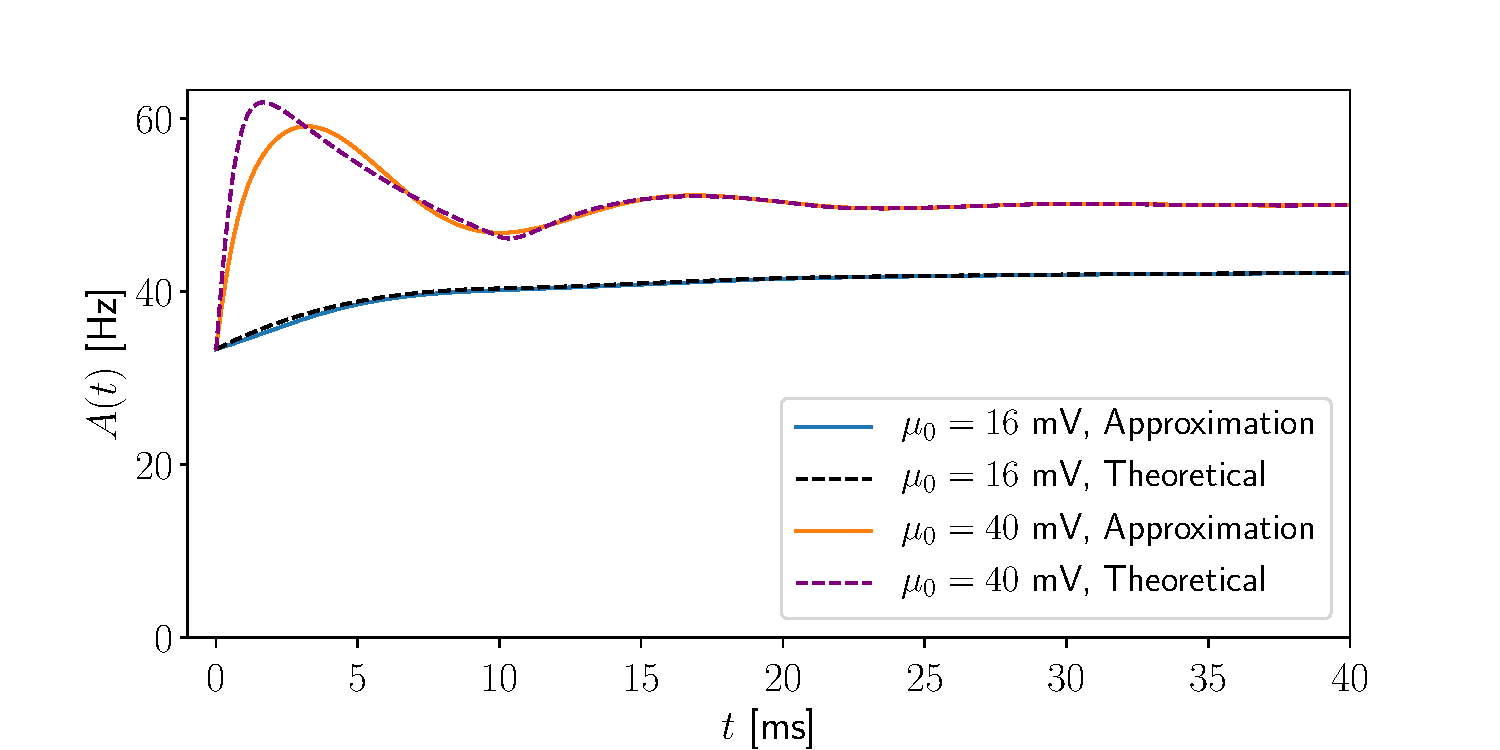
\includegraphics[width=0.8\linewidth]{Astep.pdf}
	\caption{Transient response for a population of uncoupled Poisson neurons with absolute refractoriness, receiving as external input a step function $\mu(t)$. The parameters of the neurons are $\nu_{max}=100$ Hz, $\Delta=10$ ms, $\beta=1$ mV$^{-1}$ , $h_0=15$ mV. 
	}
	\label{fig:Astep}
\end{figure}

\begin{figure}[h!]
	\centering
	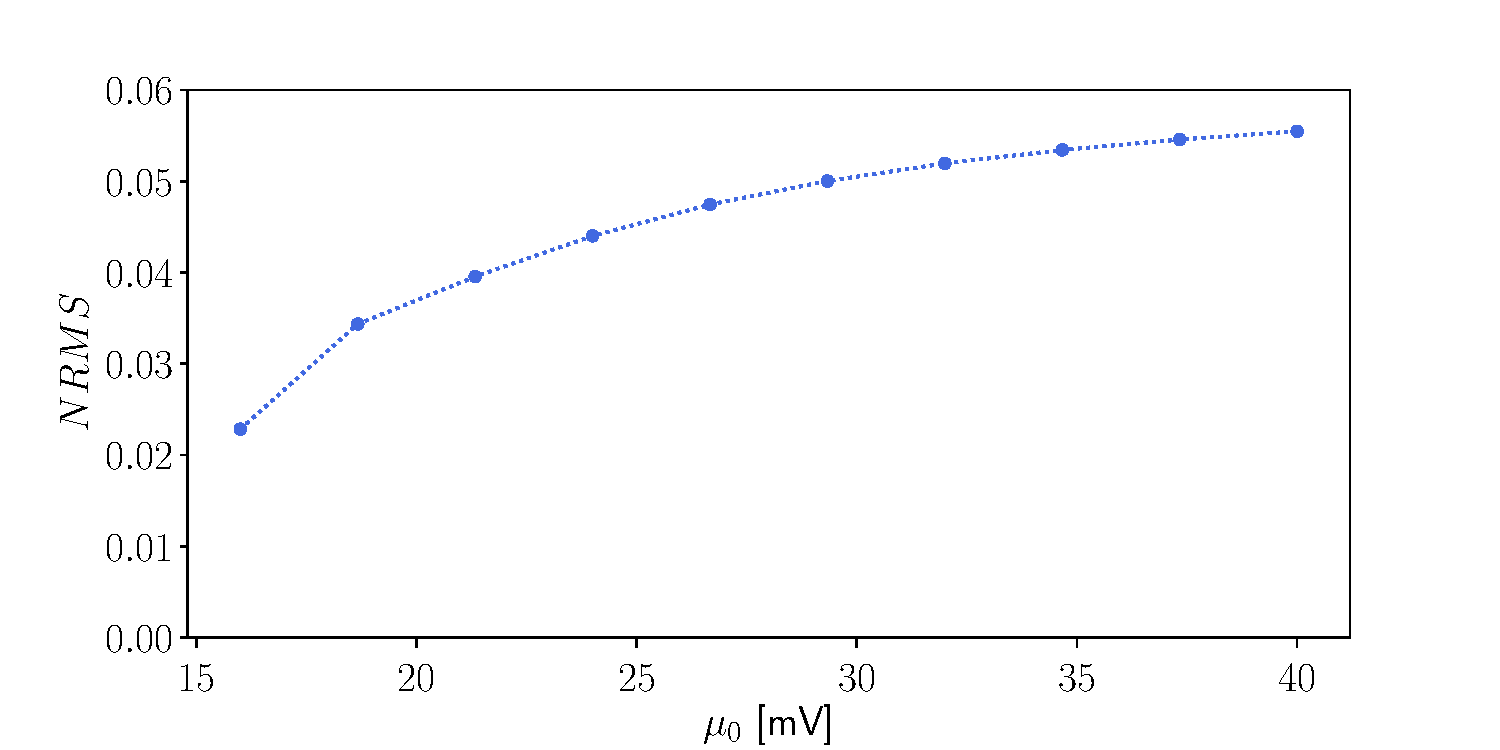
\includegraphics[width=0.8\linewidth]{NRMSstep.pdf}
	\caption{NRMS on the response of population of uncoupled Poisson neurons with absolute refractoriness to a abrupt change in the input potential $\mu(t)$. for different step from $15$ mV to $\mu_0$. The parameters of the neurons are $\nu_{max}=100$ Hz, $\Delta=10$ ms, $\beta=1$ mV$^{-1}$ , $h_0=15$ mV. The time constant of the input potential $h$ is $\tau_m=10$ ms.
	}
	\label{fig:NRMSstep}
\end{figure}

\section{Effect of the refractoriness}

To analyze the effect of the refractory period $\Delta$ on the transient response to an external input $\mu(t)$, we will compare the activity of a population of Poisson neuron with absolute refractoriness to an "equivalent" population of Poisson neuron. We know that the mean firing rate $R$ of a population of Poisson neuron with absolute refractoriness $\Delta$ is given by 

\begin{equation}
\label{eq:eqfr}
R=\frac{\Phi(h)}{1+\Phi(h)}
\end{equation}

Therefore the "equivalent" population of Poisson neurons is defined as a population of Poisson neuron with firing rate given by Eq.\eqref{eq:eqfr}.


Fig.\ref{fig:refractory_rep} illustrates the difference in the response between a population of Poisson neurons with absolute refractoriness (blue line) and an "equivalent" population of Poisson neurons (red line) to abrupt change in the input potential $\mu(t)$. the external input $\mu(t)$ was a step function changing every $50$ ms ($30$ mV / $10$ mV / $30$ mV / $16$ mV). Note that the blue line was obtained using the approximation Eq.\eqref{eq:A4}, with an $NMRS=0.02$. Contrary to the "equivalent" population of Poisson neuron, for the Poisson neurons with absolute refractoriness the response of the population activity to an abrupt change shows an oscillatory behavior in the approach to the new stationary state. The oscillations are absent in a quasi-stationary state and as expected the population activity become identical. When the input is lowered, the response of the population is delayed and doesn't show oscillations and the response of the population of Poisson neurons with absolute refractoriness is a bit faster.


\begin{figure}[h!]
	\centering
	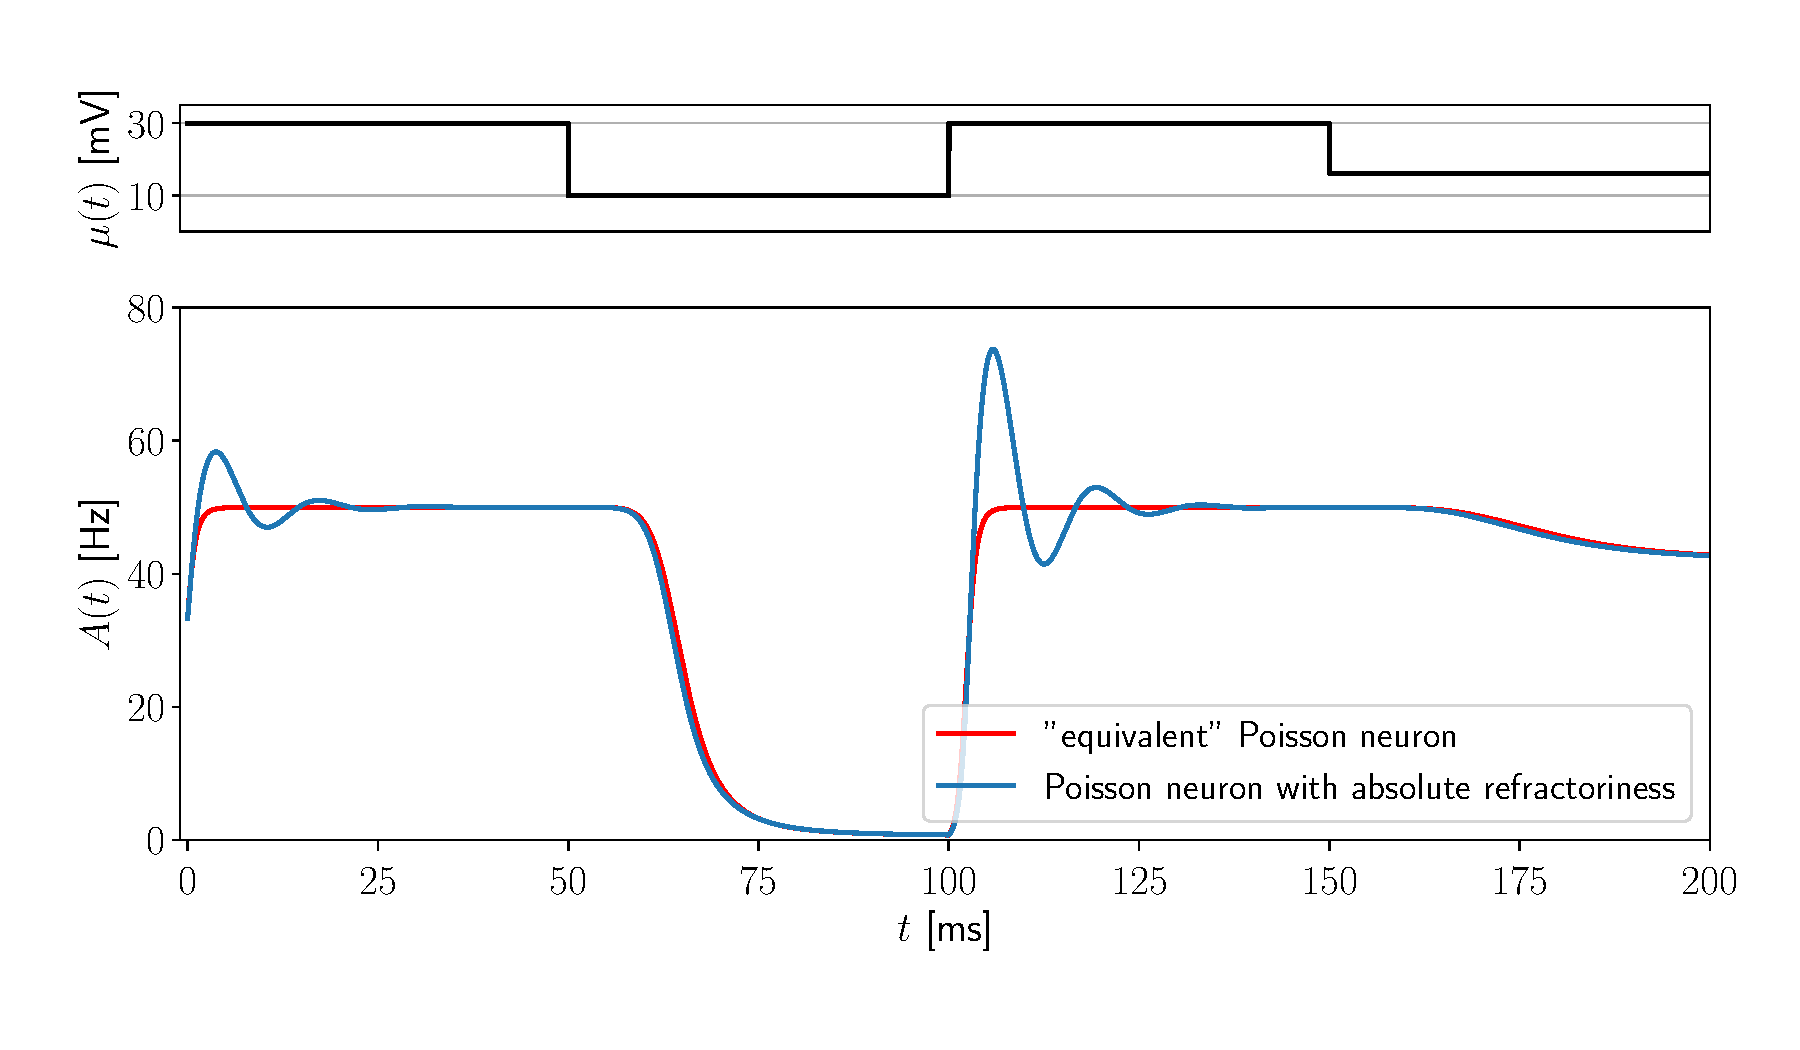
\includegraphics[width=0.7\linewidth]{refractory_rep.pdf}
	\caption{Transient response of the population activity (bottom) receiving as external input an step function $\mu(t)$ (top). The blue line correspond to the response of poisson neuron with absolute refractory period .The parameters of the neurons are $\nu_{max}=100$ Hz, $\Delta=10$ ms, $\beta=1$ mV$^{-1}$ , $h_0=15$ mV. The red line correspond to the "equivalent" population of Poisson neuron with firing rate given by Eq.\eqref{eq:eqfr}
	}
	\label{fig:refractory_rep}
\end{figure}



\chapter{Population dynamics of coupled neurons}
\label{chap:coupled}

In this Chapter we consider an all-to-all coupled population of Poisson neuron with absolute refractoriness with firing rate given by $\Phi(h)$ Eq.\eqref{eq:phi}. The dynamics of the input potential $h$ are given by

\begin{equation}
\label{eq:h2}
\tau_m\dot{h}=-h+JA(t)+\mu(t)
\end{equation}

where $\mu(t)$ is an external input potential and $J$ is the coupling constant. For the sake of simplicity for the study, we will set some of the parameters constant. The parameters of the neurons are $\nu_{max}=100$ Hz, $\Delta=10$ ms, $\beta=1$ mV$^{-1}$ , $h_0=0$ mV, and the time constant of the input potential $h$ is $\tau_m=10$ ms.


We use as an error measure the normalized root-mean-square deviation Eq.\eqref{eq:NRMS}

\section{Response to time dependent input}

In this section we analyze the response similar to time dependent input, for a coupled population of excitatory neuron, i.e $J>0$. As for the uncoupled case Section \ref{sec:uncoupletimedep} we looked at the response of the model to a sinusoidal modulation of the external input potential $\mu(t)$ with an angular frequency $\omega_s$  Eq.\eqref{eq:mut}

The input potential was initialized as if the population activity was at a stationary state with $\mu_0=-1$ mV and $J=50$ mV$\cdot$ ms.

The results are summarize in Fig.\ref{fig:NRMSo_coupled}. Just as in the uncoupled case, for high frequency the approximation becomes poor. Fig.\ref{fig:A_omega_t_coupled} illustrates the response to a sinusoidal modulation with frequency $40$ Hz.


\begin{figure}[h!]
	\centering
	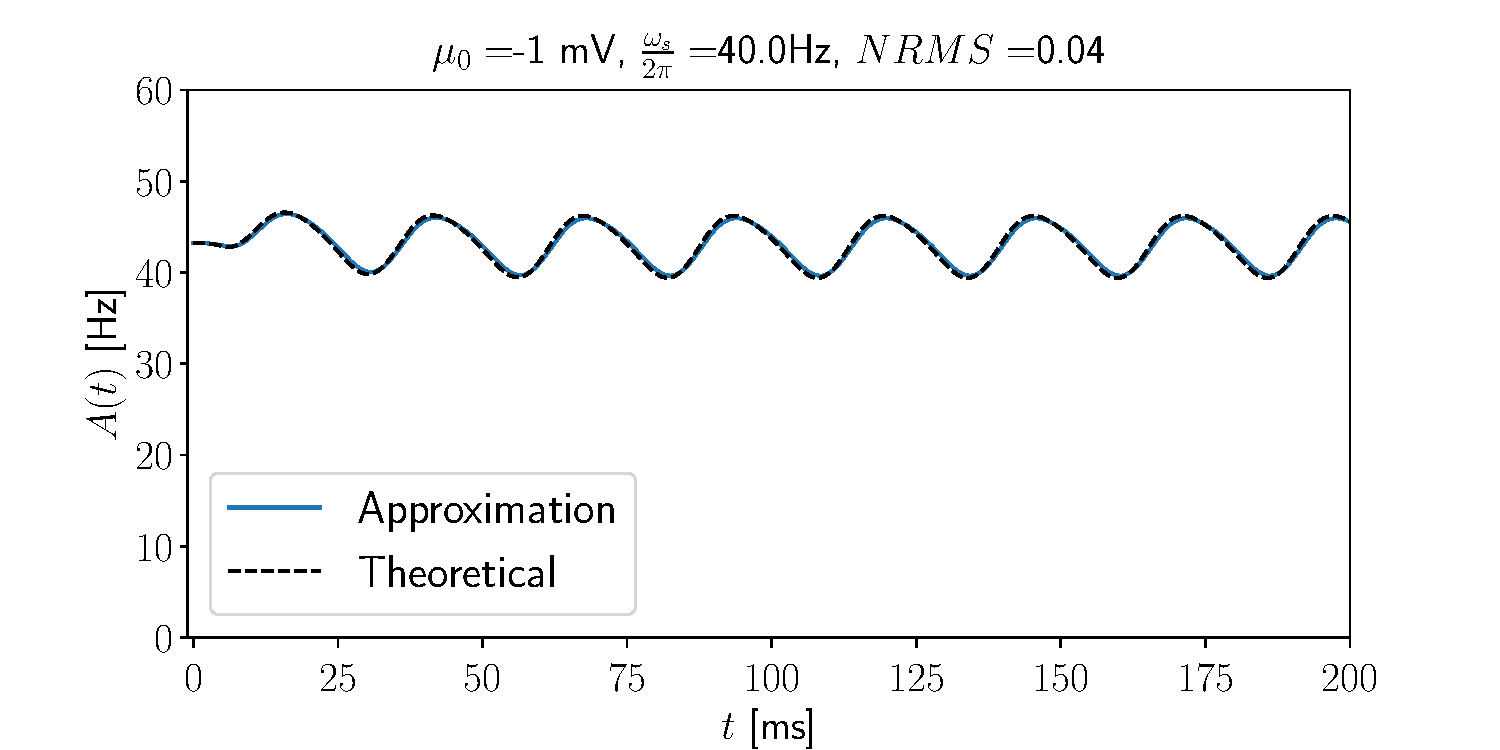
\includegraphics[width=0.8\linewidth]{A_omega_t_coupled.pdf}
	\caption{Population response to an oscillating input $\mu(t)$ with a frequency of $40$Hz, for a large populations of coupled Poisson neurons with absolute refractoriness. The parameters of the neurons are $\nu_{max}=100$ Hz, $\Delta=10$ ms, $\beta=1$ mV$^{-1}$ and  $J=50$ mV$\cdot$ ms.
	}
	\label{fig:A_omega_t_coupled}
\end{figure}


\begin{figure}[h!]
	\centering
	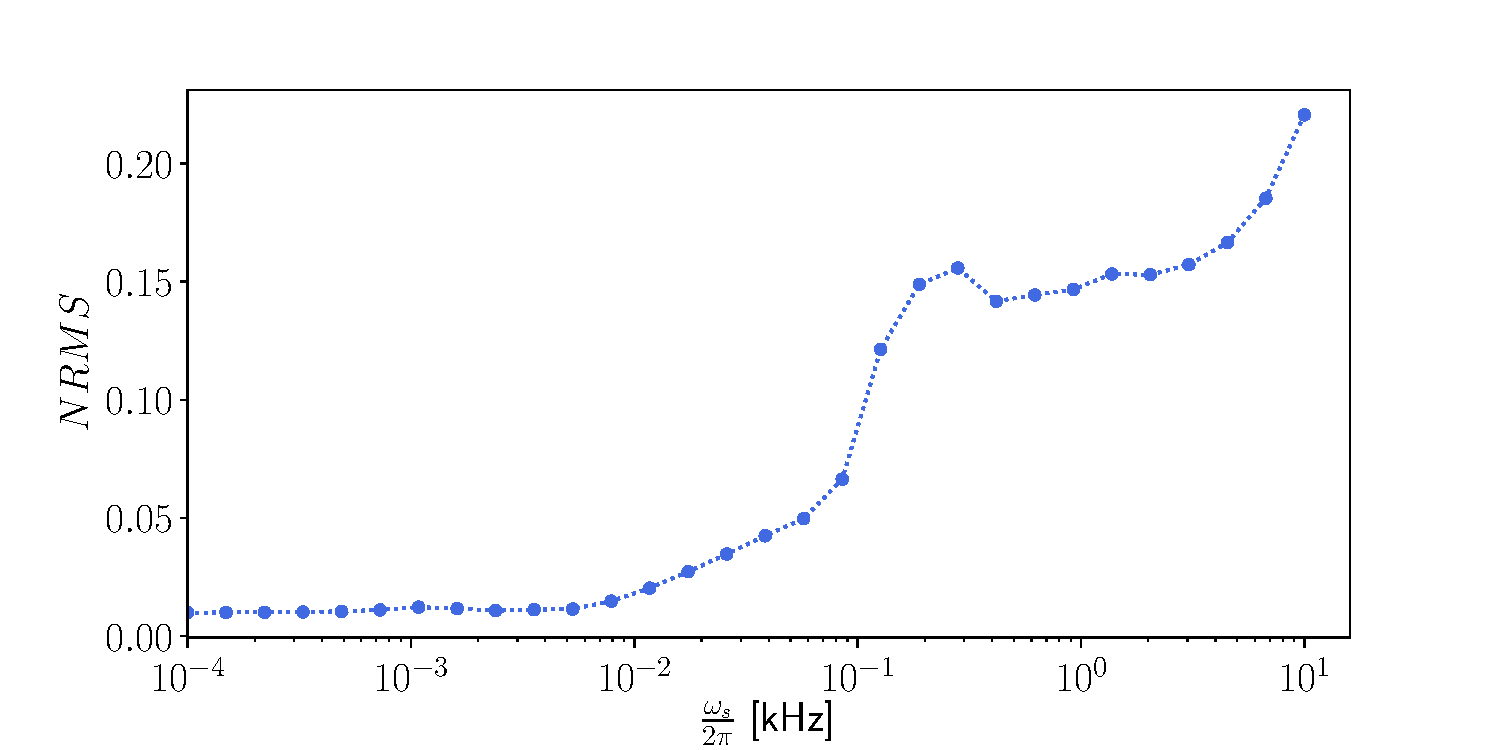
\includegraphics[width=0.8\linewidth]{NRMSo_coupled.pdf}
	\caption{NRMS on the response of population of coupled Poisson neurons with absolute refractoriness as a function of the angular frequency $\omega_s$  of the sinusoidal modulation of the external input potential $\mu(t)$ Eq.\eqref{eq:mut}. The parameters of the neurons are $\nu_{max}=100$ Hz, $\Delta=10$ ms, $\beta=1$ mV$^{-1}$ and  $J=50$ mV$\cdot$ ms.
	}
	\label{fig:NRMSo_coupled}
\end{figure}


We analyzed the response of the population activity to an abrupt change in the external input with a step function, from $\mu(0)=-2$ mV to a fixed value between $-15$ mV and $30$ mV. Fig.\ref{fig:Astep_coupled}  illustrates the response for the extreme values of the step potential $\mu(t)$. For $\mu(t)=30mV$ The response shows an oscillatory behavior, which is after $12\:$ms well approximated by Eq.\eqref{eq:A4}.  Because of the positive feedback the system goes to saturation, the firing rate $\Phi(h)$ after the refractory period $\Delta$ goes immediately to $\nu_{max}=100$Hz. With $\Delta=10ms$ this yields to a rate of $50$Hz as seen in stationary state. For the stationary state the rate is indeed given by $\frac{\Phi(h)}{1+\Delta \Phi(h)}$

%TODO W change not very well explained
 For $\mu(t)=-15mV$ the coupling is not strong enough to compensate the strong negative external potential and the activity goes to $0$. We see that the response of the approximation is a bit slower than the theoretical one. Fig.\ref{fig:NRMSstep_coupled} shows that the bigger the step in the external input potential the higher the NRMS.


\begin{figure}[h!]
	\centering
	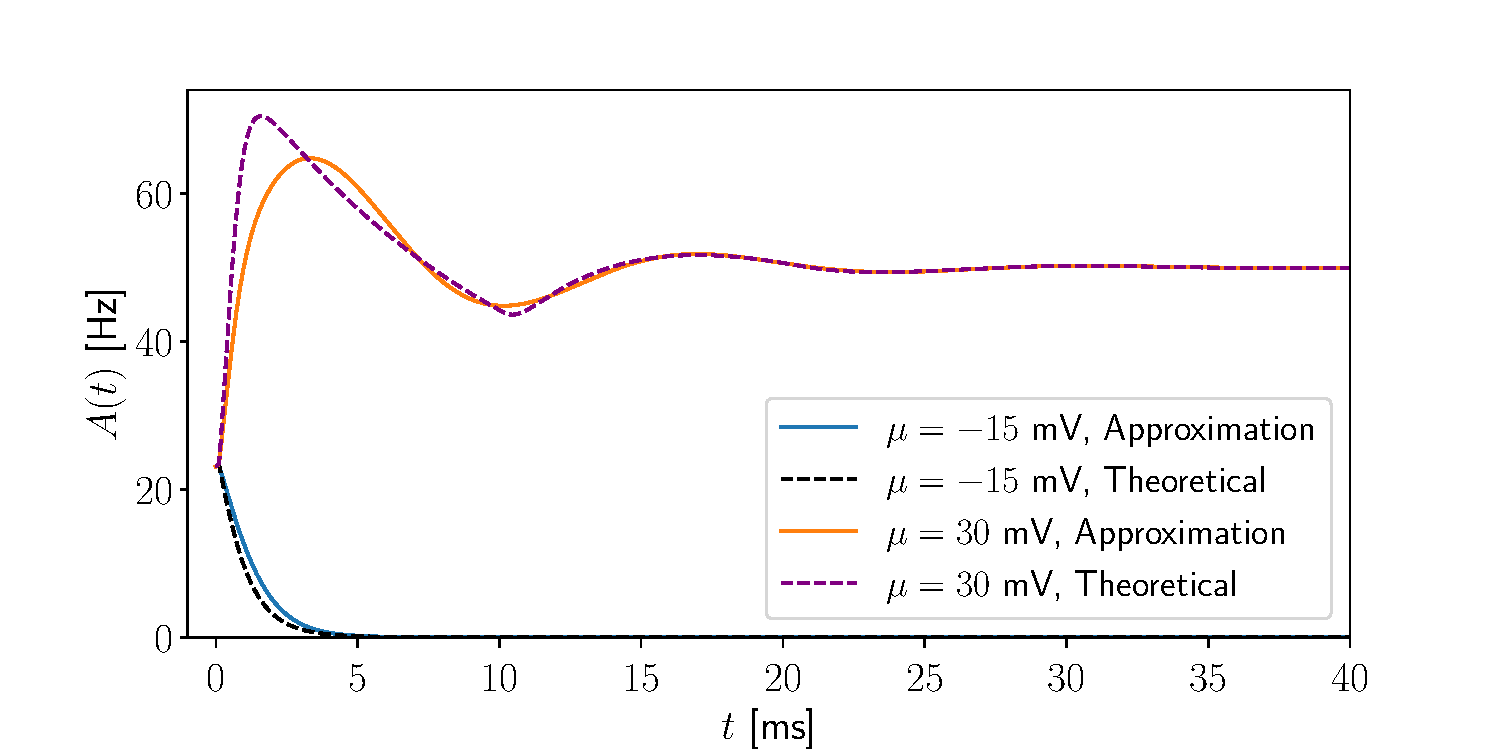
\includegraphics[width=0.8\linewidth]{Astep_coupled.pdf}
	\caption{Transient response of the population activity for a population of coupled Poisson neurons with absolute refractoriness. receiving as external input a step function $\mu(t)$. The parameters of the neurons are $\nu_{max}=100$ Hz, $\Delta=10$ ms, $\beta=1$ mV$^{-1}$ , $J=50$ mV$\cdot$ ms.
	}
	\label{fig:Astep_coupled}
\end{figure}

\begin{figure}[h!]
	\centering
	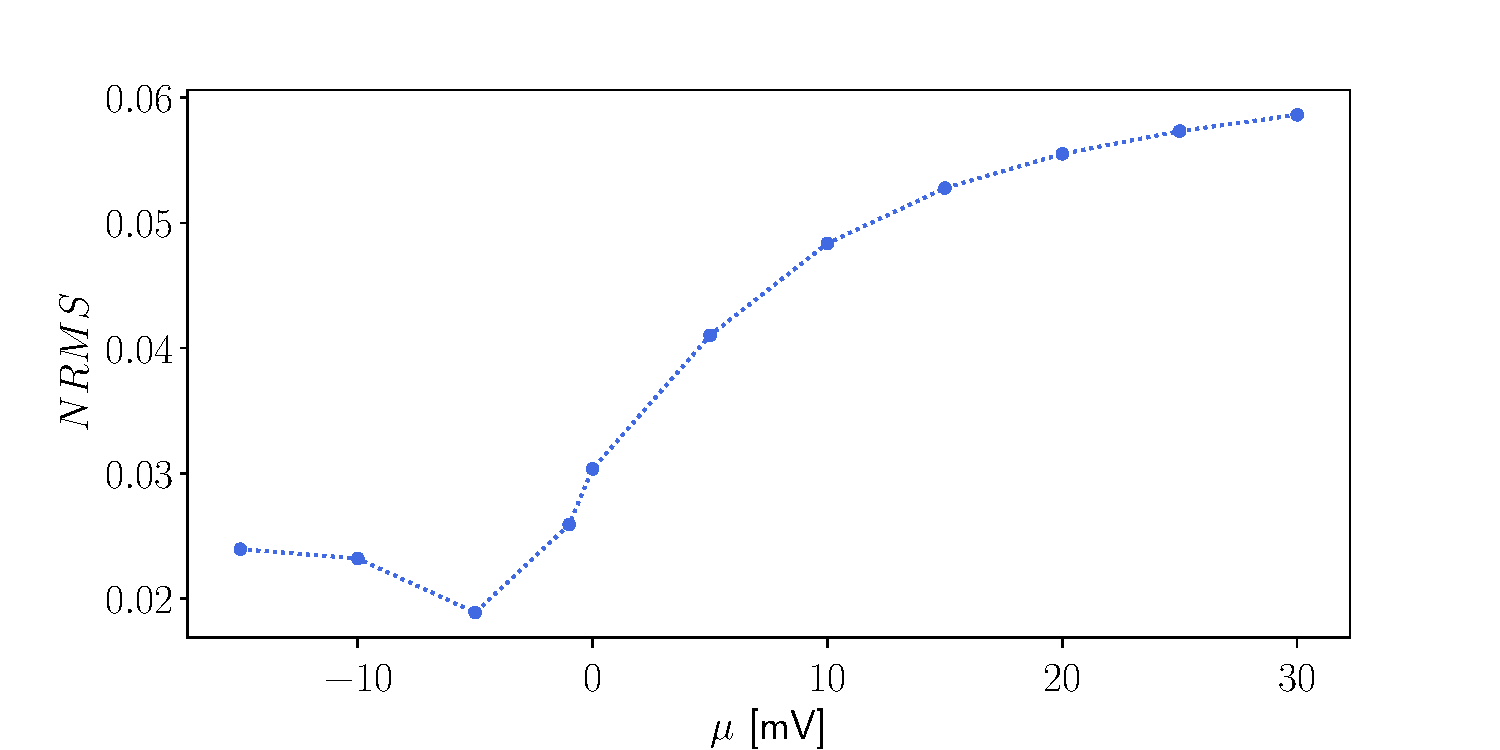
\includegraphics[width=0.8\linewidth]{NRMSstep_coupled.pdf}
	\caption{NRMS on the response of population of coupled Poisson neurons with absolute refractoriness to a abrupt change in the input potential $\mu(t)$. For different step from $-2$ mV to $\mu$,  $-15$ mV$\leq\mu\leq30$ mV . The parameters of the neurons are $\nu_{max}=100$ Hz, $\Delta=10$ ms, $\beta=1$ mV$^{-1}$, $J=50$ mV$\cdot$ ms.
	}
	\label{fig:NRMSstep_coupled}
\end{figure}


\section{Fixed points of the dynamical system} 
\label{sec:fixpoint}
In this section we are presenting preliminary results on the analysis of the fixed points of the model as a function of the coupling constant $J$ and the external constant input $\mu$. 

We have a system of three differential equation $\dot{X}$, $\dot{Y}$ and $\dot{h}$ Eq.\eqref{eq:X},\eqref{eq:Y},\eqref{eq:h2}, we are looking for the fixed point of this system. When the activity reach an stationary value, this imply that $a_1(t)=0$ an thus $X_{eq}=Y_{eq}=0$ and 


\begin{equation}
A_eq=\phi_0(0,h_{eq})=\frac{\Phi(h_{eq})}{1+\Delta \Phi(h_{eq}} 
\end{equation} 

Note that looking at Eq.\eqref{eq:X},\eqref{eq:Y}, for $X=Y=0$ and $h_{eq}$ satisfying $\dot{h}=0$ implies that $\dot{X}=\dot{Y}$=0. Therefore we can find the fixed point $h_{eq}$ solving the equation
%TODO wrong ? W change

\begin{equation}
\label{eq:hdot}
\tau_m \dot{h}=0=-h_{eq}+J\frac{\Phi(h_{eq})}{1+\Delta \Phi(h_{eq}} +\mu
\end{equation}

Fig.\ref{fig:hdyn} illustrates the solution of Eq.\eqref{eq:hdot} for different $J$. We see that for $J=250$ there are three fixed points (two stables and one unstable), but for $J=50$ and $J=-50$ there is just one stable fixed point. 

Eq.\eqref{eq:hdot} might have more than one fixed point if there are local maxima or minima. To find the condition to have more than one fixed point, one can derive Eq.\eqref{eq:hdot} with respect to $h$, this yields

\begin{equation}
\label{eq:xeq}
x^2+\left(2(1+\Delta \nu_{max}))-J\beta\right)x +\left(1+\Delta\nu_{max}\right)^2=0
\end{equation}

Where $x=\exp(-\beta(h-h_0))$. A real solutions exist for $x$ if $J>\frac{4(1+\Delta \nu_{max)}}{\beta\nu_{max}}$, indeed, $J<0$ yields to negative solutions for $x$ which is impossible as $x$ is strictly positive, and $0<J<\frac{4(1+\Delta \nu_{max)}}{\beta\nu_{max}}$ yields to complex solutions for $x$ as the discriminant of Eq.\eqref{eq:xeq} would be negative which is also impossible.

\begin{figure}[h!]
	\centering
	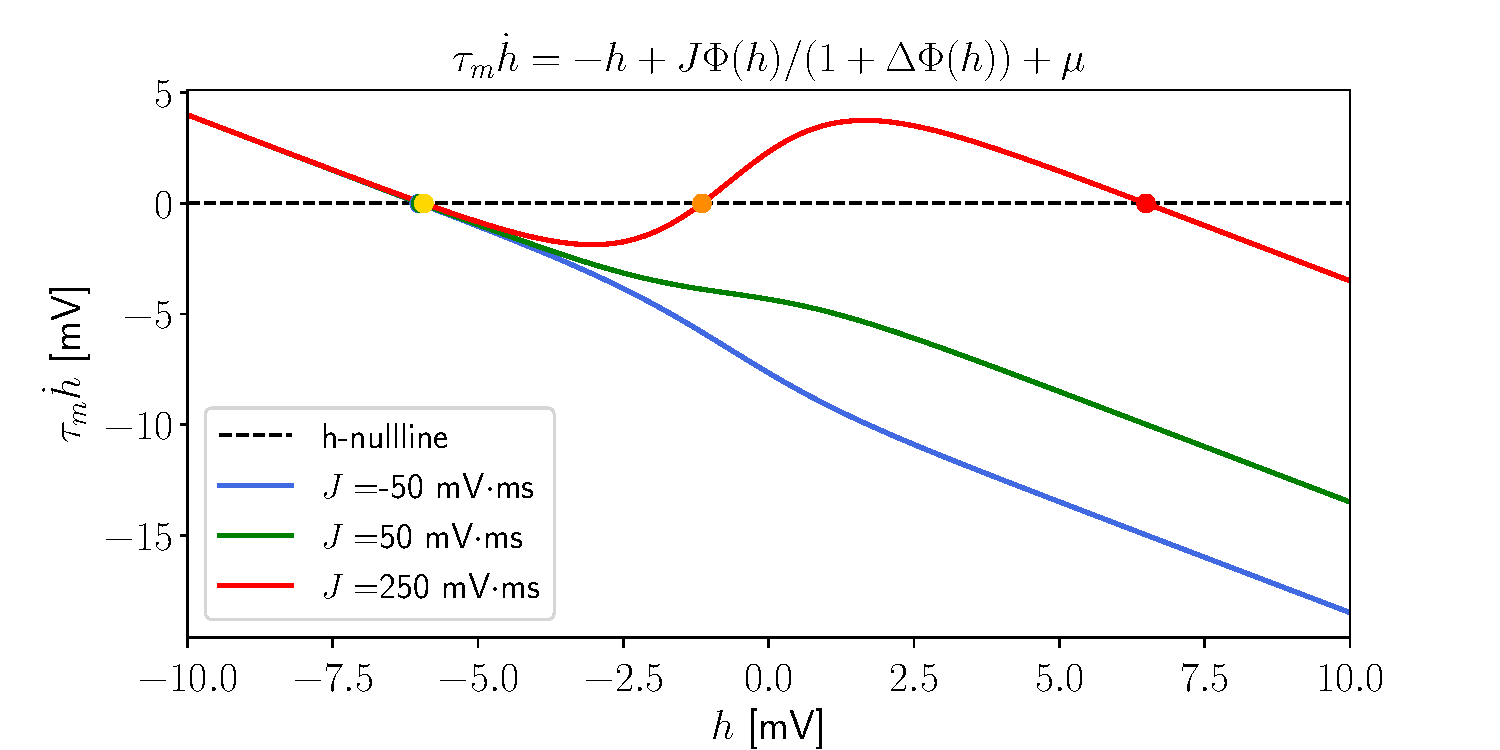
\includegraphics[width=0.8\linewidth]{hdyn.pdf}
	\caption{ $\tau_m \dot{h}$ as a function of $h$ for $mu=-6$ mV and for different J. The intersection with the $h-nullline$ corresponds to the fixed point of this dynamical system. For $J=-50$  and  $J=50$  there is only a  "low firing rate" fixed stable point respectively indicates by a blue and a green dot, they are under the yellow dot corresponding to low firing rate for $J=250$. For $J=250$ there is also an "high friring rate" stable fixed point (red dot)  and an "intermediate firing rate" unstable fixed point (orange dot).
	}
	\label{fig:hdyn}
\end{figure}

One can see on Fig.\ref{fig:hdyn} that changing $\mu$, just shift the line upward or downward. Thus for $J=250$ there is a saddle node bifurcation when we decrease or when we increase $\mu$. It is easy to compute numerically the values where the bifurcations occurs. Fig.\ref{fig:phase_plan} summarize the derivation showing the number of fixed point as a function of $J$ and $\mu$, the three dots corresponds to the pair of parameters $(J,\mu)$ used in Fig.\ref{fig:hdyn}.



\begin{figure}[h!]
	\centering
	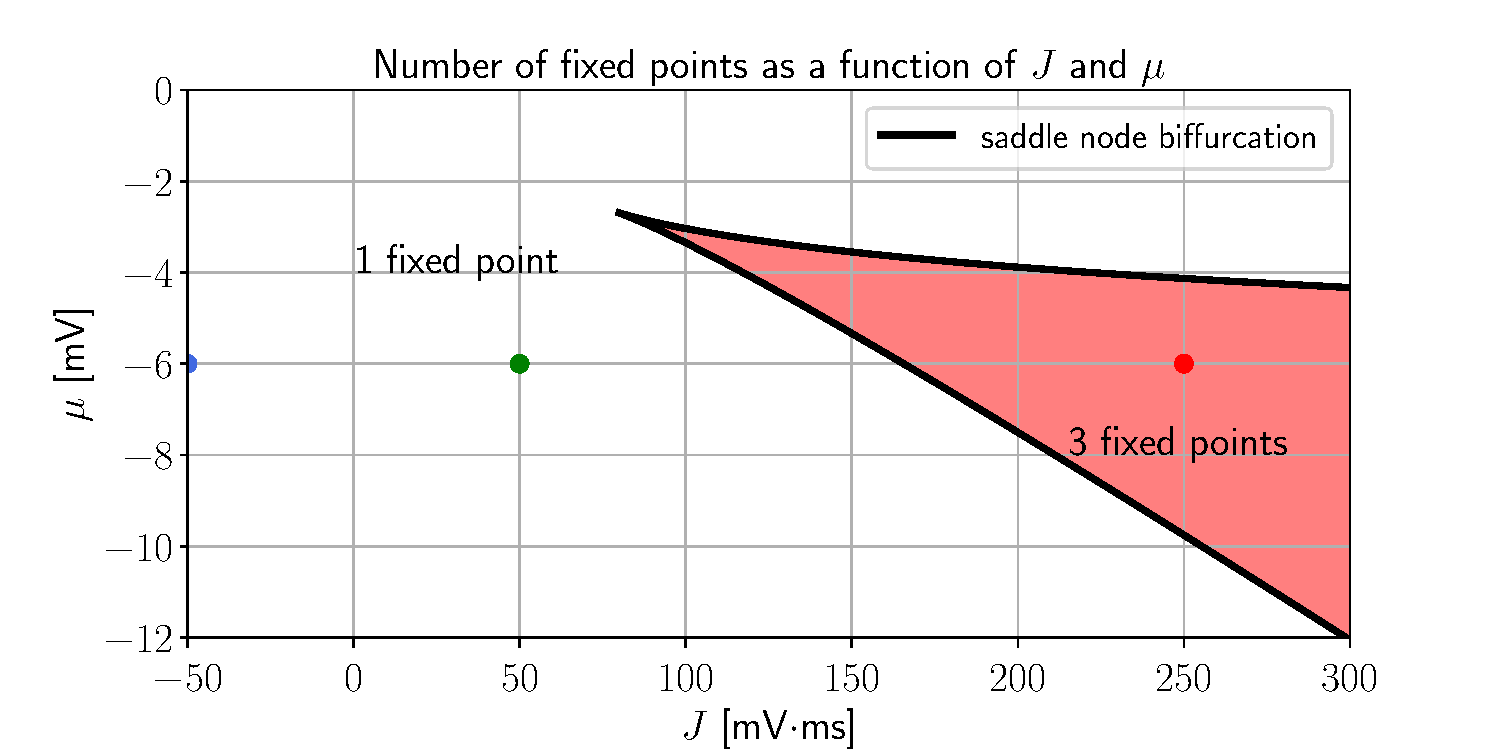
\includegraphics[width=0.8\linewidth]{phase_plan.pdf}
	\caption{Number of fixed point and bifurcation for the parameters $J$ and $\mu$. The three dots corresponds to the pair of parameters $(J,\mu)$ used in Fig\ref{fig:hdyn}.
	}
	\label{fig:phase_plan}
\end{figure}


To verify the stability of the different fixed points one can compute the Jacobian matrix of $(\dot{h},\dot{X},\dot{Y})$ evaluated in those fixed points.

\begin{equation}
J_f(h_{eq},0,0)=
\begin{pmatrix}
\partial_h \dot{h}  & \partial_X \dot{h} & \partial_Y \dot{h}  \\
\partial_h \dot{X}  & \partial_X \dot{X} & \partial_Y \dot{X}  \\
\partial_h \dot{Y}  & \partial_X \dot{Y} & \partial_Y \dot{Y}  \\
\end{pmatrix}_{|(h_{eq},0,0)}
\end{equation}

This Jacobian matrix is directly obtained differentiating  Eq.\eqref{eq:X},\eqref{eq:Y},\eqref{eq:h2} with respect to $h$, $X$ and $Y$ and using the notation introduced in Eq.\eqref{eq:first} to Eq.\eqref{eq:last}.

\begin{equation}
\label{eq:jf}
J_f=
\begin{pmatrix}
\frac{-1+J\partial_h\phi_0(0,h_{eq})}{\tau_m} & \frac{2J\Phi_r(h_{eq})}{\tau_m} & \frac{-2J\Phi_r(h_{eq})}{\tau_m}  \\
\eta_r\frac{-1+J\partial_h\phi_0(0,h_{eq})}{\tau_m} &\alpha_r(h_{eq})+\eta_r(h_{eq}) \frac{2J\Phi_r(h_{eq})}{\tau_m} & -\alpha_i(h_{eq})+\eta_r(h_{eq})\frac{-2J\Phi_r(h_{eq})}{\tau_m}  \\
\eta_i\frac{-1+J\partial_h\phi_0(0,h_{eq})}{\tau_m} &\alpha_i(h_{eq})+\eta_i(h_{eq}) \frac{2J\Phi_r(h_{eq})}{\tau_m} & \alpha_r(h_{eq})+\eta_i(h_{eq})\frac{-2J\Phi_r(h_{eq})}{\tau_m}  \\
\end{pmatrix}
\end{equation}

If the real part of the three eigenvalues of the Jacobian matrix is negative then the fixed point is stable. The different eigenvalue are represented in the complex plane in Fig.\ref{fig:eigv}. We deduce that the "low firing rate" fixed point is a stable focus for $J=50$,$J=-50$, $J=250$, for $J=250$ the "high firing rate" fixed point is also a stable focus and the "intermediate firing rate" fixed point is unstable.

\begin{figure}[h!]
	\centering
	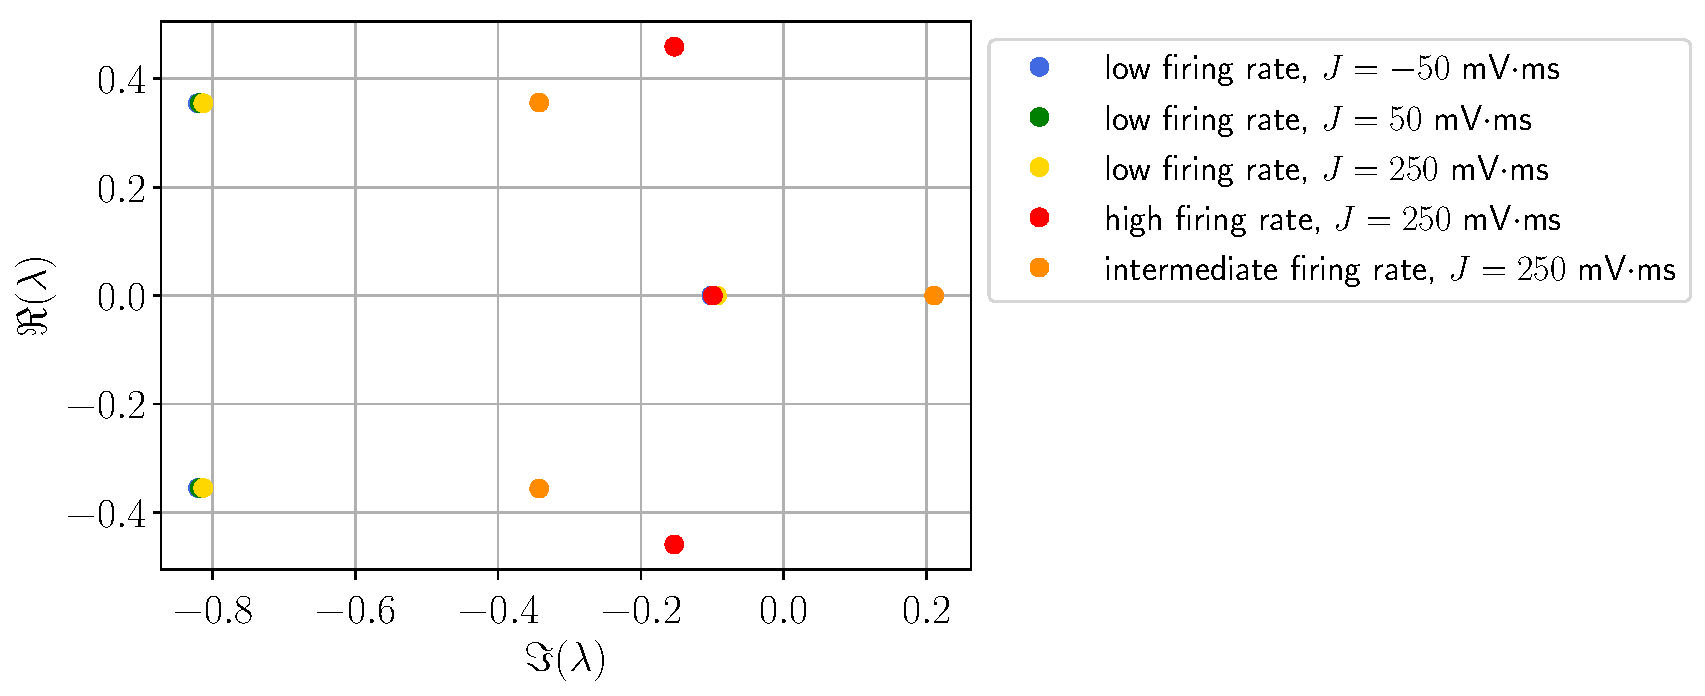
\includegraphics[width=0.8\linewidth]{hdyn_eig.pdf}
	\caption{Representation in the complex plane of the three eigenvalues of the Jacobian Matrix Eq.\eqref{eq:jf} for different fixed points. The colors of the different fixed points correspond to the fixed points in Fig.\ref{fig:hdyn}. Note that for $\Re{\lambda}\simeq-0.8$ the yellow, blue and green dots are superposed and for $\Re{\lambda}\simeq-0.1$ and $\Im{\lambda}\simeq-0.1$, the yellow, blue and green and red dots are superposed.
	}
	\label{fig:eigv}
\end{figure}


\chapter{Conclusions}

We considered a large homogeneous populations of neurons modeled by a time dependent renewal process. We applied a probability density approach, which describes the evolution of the refractory density of states $q(\tau,t)$, where the age $\tau$ of a neuron is a state variable. We applied the eigenfunction expansion method presented in Section \ref{sec:spect} to the operator of the refractory density, and derived from it a condition for the spectrum $\lambda_n$, Eq.\eqref{eq:condition2}. We also found a general expression for the biorthonormal basis of the refractory operator Eq.\eqref{eq:phin},Eq.\eqref{eq:psin}  and Eq.\eqref{eq:normalization}.
Keeping the slowest mode of the  expansion of the refractory density, we derived a three dimensional system Eq.\eqref{eq:X},\eqref{eq:Y} and\eqref{eq:h2}, and a low dimensional firing rate equation Eq.\eqref{eq:A4}. This three dimensional system has the advantages of being computationally efficient and mathematically tractable. For example in Section.\ref{sec:fixpoint} we analyzed the fixed point of the derived system, in the case of Poisson neurons with absolute refractoriness.\\

To study the accuracy of our approximation we looked at the response of population of Poisson neuron with absolute refractory period $\Delta$ to time dependent input and compare it to the theoretical solution with the integral formulation. Chapter.\ref{chap:grene} emphasizes the validity of the approximation for low frequencies in both the uncoupled case and coupled case. The response to a step function is rapidly well approximated by Eq.\eqref{eq:A4}.\\

They are nevertheless some limitations of the analytical results. For a general model defined by its hazard rate function, it's not always possible to find an analytical solution to the condition Eq.\eqref{eq:condition2}. That's why we tried to find an approximation of the first eigenvalue $\lambda_1$  as we want to keep only the two first mode. Using the cumulant expansion Section.\eqref{sec:eigv} we found an approximation which seems to be valid for low $C_V$, and is close to the one obtained in [\cite{SchOst13}], but more general. Another limitation is that it is not always possible to derive an analytical form of the eigenfunctions, especially  it is not easy to find a solution of the normalization condition Eq.\eqref{eq:normalization}, and also find an analytical form of the coupling coefficient. This has not been yet investigated, and would be a direction to continue this work. We also neglect in this model finite size effect, and the sparse coupling of neurons \cite{SchDeg17}. \\

Despite those limitations, the analytical results have many advantages. We obtained the expected response of large homogeneous population of Poisson neurons with absolute refractory period, to different external inputs potential. This simple model is very useful to study the effect of absolute refractoriness. Furthermore we derived a low dimensional firing rate dynamics of spiking neuron network from properties of individual neurons, which is not a phenomenological firing rate model. As a future work it would be interesting to use this model to analyze the interaction between different populations of excitatory and inhibitory neurons.



%

%----------------------------------------------------------------------------------------
%\printnomenclature
%----------------------------------------------------------------------------------------
\clearpage
%\addcontentsline{toc}{chapter}{References}

%\bibliographystyle{abbrv}
\bibliographystyle{abbrvnat}
%\bibliographystyle{ieeetr}
%\bibliographystyle{unsrt}
%\bibliographystyle{plainnat}
%\bibliographystyle{plain}

\renewcommand{\bibname}{References} % changes the header; default: Bibliography

\nocite{GerKis14,WilCow72,GerKis02,KniMan96,MatGiu02,Mat16_arxiv,SchOst13,Sch13,DayAbb05,Ris84,Vre10,OstBru11,AugLad17,Prij93,Lef09,KanSch00,Kni72,Ger00,ChiGra07,ChiGra08,SchDeg17}



\bibliography{my}
%\begin{thebibliography}{9}


%\end{thebibliography}

\end{document}